% Template for a Computer Science Tripos Part II project dissertation
\documentclass[12pt,a4paper,twoside,openright]{report}
\usepackage[pdfborder={0 0 0}]{hyperref}  % turns references into hyperlinks
\usepackage[margin=25mm]{geometry} % adjusts page layout
\usepackage{graphicx} % allows inclusion of PDF, PNG and JPG images
\usepackage{import}
\usepackage{docmute}  % only needed to allow inclusion of proposal.tex
\usepackage[sorting=none,backend=bibtex]{biblatex}
\usepackage[super]{nth}
\usepackage{subfig}
\usepackage{array}
\usepackage{booktabs}
\usepackage{supertabular}

\usepackage[justification=centering]{caption}% or e.g. [format=hang]
% \usepackage{showkeys}

\usepackage{amsmath}
\usepackage{amsthm}
\usepackage{txfonts}
\usepackage{lmodern}
\usepackage{proof}
\usepackage{mathtools}
\usepackage{enumitem}
\setlistdepth{20} % Magically makes the 'too deeply nested' error go away on some cases
\usepackage{array}

\usepackage{listings}
\usepackage{verbatim}
\usepackage{minted}
\usepackage{thmtools}
\usepackage{etoolbox}

\theoremstyle{definition}
\newtheorem{definition}[equation]{Definition}

\newtheoremstyle{dotless}{\topsep}{\topsep}{\itshape}{}{\bfseries}{}{5pt plus 1pt minus 1pt}{}
\theoremstyle{dotless}
\newtheorem{lemma}[definition]{Lemma}
\newtheorem{theorem}[definition]{Theorem}


\bibliography{mybib}
\raggedbottom
\sloppy
\clubpenalty1000%
\widowpenalty1000%

\usemintedstyle{friendly}
\newcommand*{\js}{\mintinline{javascript}}
\newcommand*{\orig}{\ensuremath{\!\multimapinv\!}}

\usepackage{float}
\makeatletter
\newcommand\fs@plainruled{\def\@fs@cfont{\rmfamily}\let\@fs@capt\floatc@plain%
  \def\@fs@pre{}%
  \def\@fs@mid{\kern2pt\hrule\vspace\abovecaptionskip\relax}%
  \def\@fs@post{}%
  \let\@fs@iftopcapt\iffalse
}
\patchcmd{\@thm}{\trivlist}{\list{}{ \leftmargin=1.5em\rightmargin=1.5em}}{}{}
\patchcmd{\@endtheorem}{\endtrivlist}{\endlist}{}{}
\makeatother
\floatstyle{plain}

\declaretheoremstyle[
spaceabove=6pt, spacebelow=6pt,
headfont=\bfseries, numbered=no,
notefont=\normalfont\bfseries\scshape, headpunct={\\}, notebraces={}{},
bodyfont=\normalfont,
postheadspace=1em
]{casestyle}
\declaretheorem[style=casestyle]{case}

\declaretheoremstyle[
spaceabove=6pt, spacebelow=3pt,
headfont=\normalfont\bfseries\scshape,
notefont=\normalfont\bfseries\scshape, headpunct={}, numbered=no,
bodyfont=\normalfont,
postheadspace=1em
]{subcasestyle}
\declaretheorem[style=subcasestyle, name=case]{subcase}

\setlength\partopsep{-\topsep}
\addtolength\partopsep{-\parskip}
\usepackage{chngcntr}
\newfloat{program}{thp}{lop}[chapter]
\AtBeginDocument{\counterwithin{listing}{chapter}}
\floatname{program}{Listing}
\usepackage{adjustbox}
\newcommand{\myinfer}[3]{%
  $\infer[\footnotesize\textsc{#1}]
  {#2}{
	{
	  \renewcommand{\arraystretch}{0.9}
	  \begin{tabular}{>{$}c<{$}}
		#3	
	  \end{tabular}
	}
  }$
}
\newcommand{\infertable}[1]{%
  \begin{table}[H]
  	\centerline{
  	  \begin{adjustbox}{max width=\linewidth,center}
	  	\begin{tabular}{c c}
		  #1
	  	\end{tabular}%
  	  \end{adjustbox}
  	}
  \end{table}
}
\usepackage{xcolor}
\definecolor{mintedbackground}{rgb}{0.95,0.95,0.95}

\newminted[jscript]{javascript}{
bgcolor=mintedbackground,
fontfamily=tt,
linenos=true,
numberblanklines=true,
numbersep=-12pt,
gobble=0,
frame=leftline,
framerule=0.4pt,
framesep=2mm,
funcnamehighlighting=true,
tabsize=4,
obeytabs=false,
mathescape=true
samepage=false, %with this setting you can force the list to appear on the same page
showspaces=false,
showtabs =false,
texcl=false,
}
\renewcommand{\baselinestretch}{1.1}  % adjust line spacing to make more readable
\newcommand{\typable}[2][ ]{\Gamma{}\vdash\mathtt{#2}\, |_C#1\:\Gamma#1'}
\newcommand{\typed}[2]{\Gamma{}\vdash\mathtt{#1}: #2\,|_C\:\Gamma'}
\newcommand{\transition}[6]{\langle{}\mathtt{#1},#2,#3\rangle{}\rightarrow{}\langle{}\mathtt{#4},#5,#6\rangle}
\newcommand{\indHyp}{\Phi(\Gamma, m, C, \Gamma')}
\newcommand{\indHypTwo}{\Psi(\Gamma, e, T, C, \Gamma')}
\newcommand{\var}{\textbf{var}}
\newcommand{\sub}[1]{\textsubscript{#1}}
\newcommand\eqdef{\mathrel{\overset{\makebox[0pt]{\mbox{\normalfont\tiny def}}}{=}}}
\newcommand\qdot{\mathbin{\scalebox{1.5}{.}}\enspace}
\begin{document}



%%%%%%%%%%%%%%%%%%%%%%%%%%%%%%%%%%%%%%%%%%%%%%%%%%%%%%%%%%%%%%%%%%%%%%%%
% Title


\pagestyle{empty}

\rightline{\LARGE \textbf{Christopher J.~O.~Little}}

\vspace*{60mm}
\begin{center}
  \Huge
  \textbf{Building a Gradual Type System for JavaScript} \\[5mm]
  Computer Science Tripos -- Part II \\[5mm]
  Emmanuel College \\[5mm]
  \today  % today's date
\end{center}

%%%%%%%%%%%%%%%%%%%%%%%%%%%%%%%%%%%%%%%%%%%%%%%%%%%%%%%%%%%%%%%%%%%%%%%%%%%%%%
% Proforma, table of contents and list of figures

\pagestyle{plain}

\chapter*{Proforma}

{\large
  \begin{tabular}{ll}
	Name:               & \bf Christopher J.~O.~Little             \\
	College:            & \bf Emmanuel College                      \\
	Project Title:      & \bf Building a Gradual Type System for JavaScript  \\
	Examination:        & \bf Computer Science Tripos -- Part II, May 2015  \\
	Word Count:         & \bf \input{|"./disscount.sh"}\footnotemark[1] \\
	Project Originator: & Christopher J.~O.~Little 			\\
	Supervisor:         & Dr Kathryn Gray                   \\ 
  \end{tabular}
}
\footnotetext[1]{This word count was computed
  by \texttt{detex diss.tex | tr -cd '0-9A-Za-z ' | wc -w}
}
\stepcounter{footnote}


\section*{Original Aims of the Project}

I originally aimed to define an operational semantics and typing judgement for a
small subset of JavaScript, and to use this specification to build a working
implementation of a type inference system for the language. Since it is impossible
to maintain isolation from unchecked code, I also aimed to build a source-to-source
gradual-typing compiler to inject dynamic type-checks at the boundaries of the well-typed world.
The evaluation of the specification was to take the form of a proof of type
preservation and a proof of progress, while the implementation would be evaluated
through empirical testing.

\section*{Work Completed}

The ultimate specification defined a language larger than originally planned,
including arrays and, more significantly, dynamic growth of object types by
assignment to previously undefined properties. My implementation grew
accordingly, and I was able to test it not only using my own tests, but also on
production JavaScript from Mozilla's SunSpider benchmark suite. All tests
succeeded, and I proved that the language had the properties of both type
preservation and progress.  I also developed some ideas about future
development of the project, including the addition of object inheritance via
prototypes.


\section*{Special Difficulties}

None.

\newpage
\section*{Declaration}

I, Christopher Little of Emmanuel College, being a candidate for Part II of the
Computer Science Tripos, hereby declare that this dissertation and the work
described in it are my own work, unaided except as may be specified below, and
that the dissertation does not contain material that has already been used to
any substantial extent for a comparable purpose.

\bigskip
\leftline{Signed }

\bigskip
\bigskip
\leftline{Date }

\tableofcontents

\listoffigures

\listoflistings

\newpage
\section*{Acknowledgements}

I would like to thank my project supervisor, Kathy Gray, for introducing
me to the ideas of gradual typing, and for her assistance and advice throughout.
My thanks are also due to my Director of Studies, Jonathan Hayman, for his time
and effort in proofreading the final draft.

%%%%%%%%%%%%%%%%%%%%%%%%%%%%%%%%%%%%%%%%%%%%%%%%%%%%%%%%%%%%%%%%%%%%%%%
% now for the chapters

\pagestyle{headings}
% Draft #2
\documentclass[12pt,a4paper,twoside,openright]{report}
\usepackage[pdfborder={0 0 0}]{hyperref}  % turns references into hyperlinks
\usepackage[margin=25mm]{geometry} % adjusts page layout
\usepackage{graphicx} % allows inclusion of PDF, PNG and JPG images
\usepackage{import}
\usepackage{docmute}  % only needed to allow inclusion of proposal.tex
\usepackage[sorting=none,backend=bibtex]{biblatex}
\usepackage[super]{nth}
\usepackage{subfig}

\usepackage{amsmath}
\usepackage{amsthm}
\usepackage{txfonts}
\usepackage{lmodern}
\usepackage{proof}
\usepackage{mathtools}
\usepackage{enumitem}
\usepackage{showkeys}
\setlistdepth{20} % Magically makes the 'too deeply nested' error go away on some cases

\usepackage{listings}
\usepackage{verbatim}
\usepackage{minted}
\usepackage{thmtools}
\usepackage{etoolbox}

\theoremstyle{definition}
\newtheorem{definition}{Definition}[section]

\newtheoremstyle{dotless}{\topsep}{\topsep}{\itshape}{}{\bfseries}{}{5pt plus 1pt minus 1pt}{}
\theoremstyle{dotless}
\newtheorem{lemma}{Lemma}[section]
\newtheorem{theorem}{Theorem}[section]


\bibliography{mybib}
\raggedbottom
\sloppy
\clubpenalty1000%
\widowpenalty1000%

\usemintedstyle{friendly}
\newcommand*{\js}{\mintinline{javascript}}
\newcommand*{\orig}{\ensuremath{\!\multimapinv\!}}

\usepackage{float}
\makeatletter
\newcommand\fs@plainruled{\def\@fs@cfont{\rmfamily}\let\@fs@capt\floatc@plain%
  \def\@fs@pre{}%
  \def\@fs@mid{\kern2pt\hrule\vspace\abovecaptionskip\relax}%
  \def\@fs@post{}%
  \let\@fs@iftopcapt\iffalse
}
\patchcmd{\@thm}{\trivlist}{\list{}{ \leftmargin=1.5em}}{}{}
\patchcmd{\@endtheorem}{\endtrivlist}{\endlist}{}{}
\makeatother
\floatstyle{plain}

\declaretheoremstyle[
  spaceabove=6pt, spacebelow=6pt,
  headfont=\normalfont\bfseries, numbered=no,
  notefont=\textsc, headpunct={\\}, notebraces={}{},
  bodyfont=\normalfont,
  postheadspace=1em
]{casestyle}
\declaretheoremstyle[
  spaceabove=6pt, spacebelow=3pt,
  headfont=\normalfont\bfseries,
  notefont=\scshape, headpunct={}, numbered=no,
  bodyfont=\normalfont,
  postheadspace=1em
]{subcasestyle}
\declaretheorem[style=casestyle]{case}
\declaretheorem[style=subcasestyle, name=case]{subcase}

\setlength\partopsep{-\topsep}
\addtolength\partopsep{-\parskip}
\newfloat{program}{thp}{lop}
\floatname{program}{Listing}

\renewcommand{\baselinestretch}{1.1}  % adjust line spacing to make more readable
\newcommand{\typable}[2][ ]{\Gamma{}\vdash\mathtt{#2}\, |_C#1\:\Gamma#1'}
\newcommand{\typed}[2]{\Gamma{}\vdash\mathtt{#1}: #2\,|_C\:\Gamma'}
\newcommand{\transition}[6]{\langle{}\mathtt{#1},#2,#3\rangle{}\rightarrow{}\langle{}\mathtt{#4},#5,#6\rangle}
\newcommand{\indHyp}{\Phi(\Gamma, m, C, \Gamma')}
\newcommand{\indHypTwo}{\Psi(\Gamma, e, T, C, \Gamma')}
\newcommand{\var}{\textbf{var}}
\newcommand{\sub}[1]{\textsubscript{#1}}
\newcommand\eqdef{\mathrel{\overset{\makebox[0pt]{\mbox{\normalfont\tiny def}}}{=}}}
\newcommand\qdot{\mathbin{\scalebox{1.5}{.}}\enspace}
\begin{document}

\chapter{Introduction}\label{introduction}

Types are a way of grouping together values which support similar operations.
For example, \texttt{number} might be a type representing values which support
addition and subtraction. \texttt{string} might represent a sequence of
characters which supports concatenation, but doesn't support addition or
subtraction. A program in a language with these types cannot subtract a
\texttt{number} from a \texttt{string}, and an attempt to do so is known as a
\textit{type error}. We say that a language is \textit{strongly} typed if such
attempts will always generate some kind of error, whereas a \textit{weakly}
typed language may allow the operation to execute, with sometimes
unpredictable consequences. Under \textit{dynamic} typing, checking for type
errors happens at the very last minute -- during program execution itself.
Using a \textit{static} type checker, the program code can be analysed in
advance to identify type errors before the program runs.

JavaScript is a high-level, dynamically-typed programming language which was
originally designed for little more than validating forms on websites. Today
the language is an essential part of everyday computing, powering demanding
online applications such as image editors, IDEs and online games. The
execution context of the language has also changed, moving from the browser to
the server, and now even being targeted by other languages'
compilers~\cite{asm}. As the scale of JavaScript applications has increased,
so too has the complexity of development projects. Assurance that a program is
bug-free has become more critical, both for online companies which rely on
JavaScript for e-commerce, and for the people that use their applications. A
security bug in an online banking application, for example, could be
devastating. JavaScript's weak typing discipline, however, makes it hard to
reason about a program's correctness, and limits the information available to
development tools. This problem is exacerbated by JavaScript's type
\textit{coercion}, which permits expressions which would normally be deemed
untypable by, for example, converting any object to the value \js{true} when
placed in a context expecting a boolean. This can result in silent propagation
of type errors, providing no errors to the developer.

Static type checking catches potential bugs earlier in the development cycle,
Static type checking catches potential bugs earlier in the development cycle,
and can allow programs to run faster, without needing to check types before
every operation. However, it is impossible for a static type checker to
precisely identify all potential type errors, because it cannot know precisely
what the program will do when it runs. If such a type checker existed, it could
be used to determine whether any given program will terminate or not -- which
would violate the undecidability of the halting problem. Instead, a
conservative approximation is made, and some programs which would never
actually exhibit a type error will fail a static type check. This approximation
can be frustrating for developers, who will need to satisfy the type checker by
rewriting their code before it will run.

Although languages are often described as being statically or
dynamically-typed, in reality it is compilers and interpreters which enforce a
particular discipline. A compiler for a traditionally statically-typed language
could skip the static type checking phase and insert dynamic type checks
instead. In the other direction, it is sometimes possible to perform static
analysis of a program's code in order to avoid reliance on delayed runtime
checks.

Several such attempts have been made to perform static analysis on JavaScript,
which is typically a dynamically-typed language. ECMAScript~4~\cite{es4},
a proposed extension to the JavaScript standard, featured optional type
annotations, but the proposal was never finalised and the annotations are not
present in later versions of the standard. TypeScript~\cite{ts}, uses a
superset of JavaScript syntax with similar annotations, and compiles this back
into JavaScript. These approaches have depended on programmer-inserted type
annotations, which limit their utility for legacy codebases. Some projects
have attempted to use Hindley-Milner style analysis to infer the types of
program expressions automatically~\cite{anderson06, tajs, guha}, including the most
recent contribution, Flow~\cite{flow}. 

Any static analysis, however, will struggle to offer reliable results because
of the inherently dynamic nature of the language. Many traditional JavaScript
programming idioms are legitimately untypable. JavaScript has no
mechanism for overloading functions, for example, so many developers write
functions expecting different parameter types from call-to-call, and use manual
type checks to handle them (see listing~\ref{lst:dynamicIdiom}). Flow and
TypeScript allow for untypable functions using a special `any' type, which will
never trigger a static type error. The obvious disadvantage here is that the
static analysis can no longer make any guarantees about the soundness of the
program, as certain parts of it have effectively not been checked.
\begin{program}[t]
  \begin{minted}[linenos,numbersep=-12pt]{javascript}
 	// adapted from the Prototype library
 	function serialize(val) {
	  switch (typeof val) {
		case "boolean":
		return val ? "true" : "false";
		case "number":
		return "" + val;
		case "string":
		return val;
	  }
 	}	
  \end{minted}
  \label{lst:dynamicIdiom}
  \caption{Dynamic idioms in JavaScript}
\end{program}
Additionally, JavaScript code rarely operates in isolation in modern web
applications. Even if a program passes the static type checker, some external
piece of code may introduce a type error by, for example, passing data of the
incorrect type to a well-typed function.

Gradual typing is a technique used to make safety guarantees about code which
combines both static and dynamic typing. Initially looking at interoperation
between static and dynamic languages~\cite{gray2005fine}, the concepts are
also applicable here, where the division between static and dynamic code lies
within one language rather than between several. Since static analysis cannot
guarantee that the program is free of dynamic type errors, we instead
guarantee that only dynamic properties of the code are able to cause runtime
errors -- that the well-typed code ``can't be blamed"~\cite{cantblame} for
any type errors which arise. This is achieved by protecting the boundaries
between the type-safe and type- unsafe `worlds'. Conversions are made from
dynamic types to static types, and although this conversion process may
generate an error (for example trying to convert a \texttt{number} to a
\texttt{string}), the type safety of the well- typed world is provably
preserved.

In this project, I have defined a formal operational semantics and a type
system for a subset of JavaScript, and created a proof that the system defined
has the properties of \textit{progress} and \textit{type preservation}. I have
successfully implemented type inference according to this specification in
order to create a static type checker, and this implementation has been checked
by a large suite of tests. In doing this, I realised that the subset of
JavaScript initially planned to be supported was insufficient for `real-world'
code, and added arrays and object growth to both the specification and
implementation. This enabled me to test my implementation using seven tests
from the Mozilla SunSpider JavaScript benchmark suite. The only extension task
left incomplete is the inclusion of object inheritance via object prototypes,
but I present a starting point to this, which could fruitfully be built upon in
future work.

\chapter{Preparation}\label{preparation} \section{Background}

Before development could begin, an understanding of the theoretical
underpinnings of the project was required. Several of the undergraduate courses
offered as part of the Tripos were a valuable introduction, notably the Part IB
course \textit{Semantics of Programming Languages}, and the Part II courses
\textit{Types} and \textit{Optimising Compilers}. \textit{Semantics of
  Programming Languages} introduced the proof techniques necessary for proving
type soundness, but for an insufficiently complex example language to cover all
strategies required. Pierce's \textit{Types and Programming
  Languages}~\cite{pierce} bridged this gap sufficiently that I was able to look
at recent work defining the operational semantics of real dynamic programming
languages~\cite{pythonOpSem}. The \textit{Types} course similarly introduced
the Hindley--Damas--Milner algorithm for type inference, and Pierce's book
helped develop those ideas further. Neither course touched on the topic of
gradual typing, which is very much a topic of current research interest. A few
papers by Siek~\cite{gradSiek, gradSiek2} and Gray~\cite{gradGray} proved
sufficiently accessible, however, for me to explore the area.
\textit{Optimising Compilers} presented techniques for control flow analysis,
which usefully complement the inference-based analyses, for example by checking
that a variable has been defined before use.

In relation to JavaScript itself, I began the project with a strong informal
grasp of the language. The ECMAScript 5 specification~\cite{ecmaSpec} offered a
more rigorous definition, which would be required in defining my own
operational semantics. Some work has already been done attempting to formalise
the semantics of JavaScript~\cite{guha2010essence}, providing useful inspiration in designing my own
operational semantics. Carrying out any kind of static analysis on a dynamic
language will result in false negatives, where a safe statement is incorrectly
deemed unsafe. This is preferable to a false positive in terms of guaranteeing
safe operation of the program, but still frustrating for the developer. It can
be important, therefore, to understand the manner in which a language is
actually used. There is little benefit in devising solutions to the problem of
typing dynamic idioms which are hardly ever used, and so I looked through the
results of Richards, Lebresne, Burg and Vitek~\cite{JSBehaviour}, who have
analysed the dynamic behaviour of real JavaScript programs in operation on the
internet. Finally, it was educational to look at
TypeScript~\cite{ts,understandingTS}, to learn from the decisions the
TypeScript team had made, the solutions they had already found, and to fully
understand the limitations of their solution. I also attended a talk on Flow by
one of the authors, with similar ambitions.

\section{Development Plan}

The project consisted of four discrete tasks: designing a formal specification
to describe the operational semantics and type judgements for my subset,
proving that the subset as specified was sound and implementing both the type
inference system and the gradual typing compiler. Orthogonally to this, the
language was divided into discrete features, such as if-statements, binary
operations and loops. This division meant the project lent itself to an
incremental build model, whereby each build increment introduced a new language
feature to the specification, proof and implementations. This allowed
development to proceed systematically, offering sensible opportunities for
regression testing after each iteration, with only few changes since the last
test. This strategy also minimised development risk by allowing me to cease
development at the end of any iteration and still have a successful system,
albeit supporting fewer features than planned.

I used Git for version control, with the primary repository hosted on GitHub
which also served as a remote backup of my work. To amplify the benefit of my
regression tests for bug detection, I set up continuous integration such that
each time the GitHub repository was updated, the code was downloaded to a
private VPS, and the full test suite ran automatically. If any tests failed, an
email warning was sent to me, so I was immediately alerted of the problem I had
introduced, and could fix it while the changes which had triggered it were
still fresh in my mind. If all tests passed, the new code was deployed to a web
server, such that a live demo was always accessible online at
\href{http://jstyper.clittle.com}{http://jstyper.clittle.com}.

Within each iteration, I began with the specification, as a kind of
requirements analysis. The specification was written using
Ott~\cite{sewell2007ott}, a tool which I learnt to use as the project
progressed. The iteration would be considered complete when each of the other
components conformed to the specification. For the two development tasks, I
proceeded in a test-driven manner, whereby I would first write tests involving
the new language feature, expecting them to fail. Development then aimed to
make these failing test-cases pass. My collection of tests available for
regression testing (and later for benchmarking) thus grew consistently across
the project life-cycle, and by the end of the project 
\input{|"ls ../../src/tests/custom/results -l | wc -l"}such tests had been produced.

Many developers view theoretical computer science as carrying little practical
benefit for them, when the truth is that concrete implementations of the theory
can bring huge practical benefits. It was thus important to me to integrate
smoothly within the existing JavaScript ecosystem rather than enforce a
non-standard workflow for JavaScript developers, thereby reducing the barriers
to entry and making the benefits of static typing more easily discoverable.
Languages like OCaml, although commonly used for this kind of project within
the academic community, are unlikely to be present on a web developer's
computer. Indeed, this is a problem Chaudhuri mentioned having for Flow, which
has been released as an open source project but suffers from a lack of
contributors because the project's main users are not able to understand or
make meaningful contributions to the type checker's code. Instead, I decided to
write the type inference system in JavaScript, thus ensuring it could run on
any system. This decision opened the door for writing a self-hosting compiler,
which could type-check and compile its own source code. It also potentially
made it possible for type checking and compilation to happen in the browser,
though in practice this is likely only advantageous in fairly unusual
circumstances. Instead, development focussed on running the compiler using
Node.js~\cite{nodejs}, a JavaScript interpreter designed for use outside the browser.

As an interpreted language, JavaScript is not compiled prior to execution, but
it is often compressed to speed up download times to client computers. A number
of static analysis tools exist to aid with this, performing mainly control-flow
analyses to, for example, eliminate unused variables from the source code
(known as \textit{minification}). Although I was not interested in such
analyses, it seemed sensible to integrate with a standard abstract syntax tree
(AST) format, and use existing parsing and code-generation solutions.
UglifyJS~\cite{uglify} is one of the most-used minification libraries for
JavaScript, and has separate components for parsing and code generation but
uses a custom (albeit well-documented) AST format. Esprima~\cite{esprima} is
another JavaScript parser which is marginally faster and uses the SpiderMonkey
AST format standardised by Mozilla. Various analysis tools and code generators
exist for this format, but I decided that the UglifyJS format was actually more
useful for my purposes, and parse speeds was not a priority. For example, the
SpiderMonkey AST has a single representation of any unary expression, when in
practice it can be useful to distinguish between prefix and suffix expressions.
Additionally, UglifyJS uses object inheritance to define its node types, where
Esprima prefers plain objects. 

\chapter{Implementation}\label{implementation}

There were two components to implement for the project -- the formal
specification of the language and the executable type inference system itself.
The language I specified was a subset of JavaScript, chosen to be expressive
enough to represent actual JavaScript programs while being free of some of the
complications of implementation. For example, storage of variables was
simplified to just a scope and a heap, without modelling the special cases of
the global scope, nor worrying about removal of unused data by the garbage
collector. 

\section{Language Definition}

\begin{lstlisting}[mathescape, escapechar=£]
  v            ::= $b$ | $n$ | $str$ | £\textbf{undefined}£ | £\textbf{null}£ | £\textbf{\{}£$l_1$:$v_1$, $\dots$, $l_i$:$v_i$£\textbf{\}}£
  | £\textbf{[}£$v_1$, $\dots$, $v_i$£\textbf{]}£ | £[\![£$func$, s£]\!]£
  func         ::= £\textbf{function}£ $id$£\textbf{(}£$x_1$, $\dots$, $x_i$£\textbf{)}£ £\textbf{\{}£ $m$ £\textbf{\}}£ 
  | £\textbf{function}£ £\textbf{(}£$x_1$, $\dots$, $x_i$£\textbf{)}£ £\textbf{\{}£ $m$ £\textbf{\}}£
  e            ::= $v$ | $id$ | $e$ $op$ $e'$ | £\textbf{\{}£$l_1$:$e_1$, $\dots$, $l_i$:$e_i$£\textbf{\}}£ 
  | £\textbf{[}£$e_1$, $\dots$ $e_i$£\textbf{]}£ | $e$£\textbf{.}£l | $e$£\textbf{[}£$e'$£\textbf{]}£ 
  | $e$£\textbf{(}£$e_1$, $\dots$, $e_i$£\textbf{)}£ | $func$
  | $assignTarget$ $\approx$ $e$ | $assignTarget$ $assignOp$ 
  | $assignOp$ $assignTarget$ | $preOp$ e
  m            ::= $e$ | $m_1$; $\dots$; $m_i$ | £\textbf{var}£ $vd_1$, $\dots$ $vd_i$ 
  | £\textbf{if}£ £\textbf{(}£$e$£\textbf{)}£ £\textbf{\{}£$m_1$£\textbf{\}}£ | £\textbf{if}£ £\textbf{(}£$e$£\textbf{) \{}£$m_1$£\textbf{\} else \{}£$m_2$£\textbf{\}}£ | £\textbf{while}£ £\textbf{(}£$e$£\textbf{)}£ £\textbf{\{}£$m$£\textbf{\}}£ 
  | £\textbf{for}£ £\textbf{(}£$e_1$; $e_2$; $e_3$£\textbf{)}£ £\textbf{\{}£$m$£\textbf{\}}£ | £\textbf{for}£ £\textbf{(}£$varDec$; $e_2$; $e_3$£\textbf{)}£ £\textbf{\{}£$m$£\textbf{\}}£ 
  | £\textbf{@def function}£ $id$£\textbf{(}£$x_1$, $\dots$, $x_i$£\textbf{)}£ £\textbf{\{}£$m$£\textbf{\}}£
  | £\textbf{return}£ $e$ | £\textbf{return}£  | £\textbf{$\epsilon$}£
  assignTarget ::= $vRef$ | $assignTarget$£\textbf{[}£$e$£\textbf{]}£ | $assignTarget$£\textbf{.}£l
  vRef         ::= $id$ | $vRef$£\textbf{.}£l | $vRef$£\textbf{[}£$n$£\textbf{]}£
  vd           ::= $id$ | $id$£\textbf{=}$e$£
  op           ::= $numOp$ | $cmpOp$ | $numcmpOp$ | $boolOp$
  $\approx$             ::=  £\textbf{=}£ | $numOp$£\textbf{=}£
  numOp        ::= £\textbf{+}£ | £\textbf{-}£ | £\textbf{/}£ | £\textbf{*}£ | £\textbf{\%}£
  numcmpOp     ::= £\textbf{\textless}£ | $\mathbf{\leq}$ | £\textbf{$\geq$}£ | £\textbf{\textgreater}£
  cmpOp        ::= £\textbf{===}£ | £\textbf{!==}£ | £\textbf{==}£ | £\textbf{!==}£
  boolOp       ::= £\textbf{||}£ | £\textbf{\&\&}£
  preOp        ::= £\textbf{-}£ | £\textbf{!}£
  assignOp     ::= £\textbf{-\,-}£ | £\textbf{++}£
\end{lstlisting}


The subset includes primitive constants; object and array literals;
arithmetic and logical binary and unary operators; dereferencing from and
assignment to object properties and array elements; functions and function expressions; and basic control flow via \js{if ... else ...} and loops.  
Where features of JavaScript were omitted, they largely tended to be features
which could be desugared into supported features -- for example \js{switch}
statements can be written as a series of \js{if} statements, and do not present
an interesting problem from a typing perspective. No attempt was made to
include a representation of commonly used JavaScript objects, such as the
\js{RegExp} object or elements of the \textit{Document Object Model}, which is used to
represent the structure of an HTML document. The type signatures of such objects
could be predefined for use within the system.

Some other features were excluded which would introduce difficult problems in
ensuring type safety.  Although I included the ability to dynamically grow an
object by assigning to an undefined property, I excluded the ability to remove
or change properties once defined. These features, although legal in
JavaScript, make it difficult to reason about the type safety of a property
access without control flow analyses keeping track of precisely which
properties are well-defined at each program point. Another example is the
concatenation of strings using \js{+}, which overloads the use of the \js{+}
operator to represent more than one method signature. Even where a feature is
missing, however, the gradual typing mechanism usually allows code fragments
relying on these features to bypass the type checker.

\section{Formal Specification}

The specification of my JavaScript subset has two components -- a definition of
the operational semantics, and a definition of the typing judgement used. The
executable type inference system has the job of verifying that the initial
program, as typed by the developer, is well-typed. If the specification is
correctly defined, this property can then be proved to be preserved throughout the
execution of the program.

\subsection{Operational Semantics}
The operational semantics takes the form of {\color{red}60} inductive rules
describing all possible transitions from one step of computation to another. A
step of computation is described by a configuration triple of the form
$$\langle m, s, \theta\rangle.$$ $m$ is the program code remaining to be
executed, $s$ represents the current scope (the set of variables accessible at
this program point); and $\theta$ represents the heap, where variable values
are stored.
$$\infer[\textsc{Seq2}]
{\langle \mathtt{m_1; m_2; \dots; m_i}, s, \theta\rangle \rightarrow \langle \mathtt{m_1'; m_2; \dots; m_i}, s, \theta\rangle}
{\langle\mathtt{m_1}, s, \theta\rangle\rightarrow\langle \mathtt{m_1'},s, \theta\rangle}$$

A transition rule is described by a series of premises, which, if true,
indicate that the conclusion must also be true. For example, the rule
\textsc{Seq2} tells us that, if some statement $m_1$ can reduce to $m_1'$ using
the store $(s,\theta)$, then it must also be possible to reduce any sequence of
statements beginning with $m_1$ with the same effects on the store. Most of the
rules follow an intuitive understanding of JavaScript's execution semantics, in
terms of evaluation of subexpression before evaluating the entire expression. A
few points are worth further discussion, however.

\begin{program}[t]
  \begin{minted}[numbersep=-12pt,linenos]{javascript}
	function makeCounter(n) {
	  var i = n;
	  return function() {
		if (i>0) {
		  i--;
		}
		return i;
	  }
	}

	var count = makeCounter(10);
	count(); // i is now 9, but the current scope is unchanged
  \end{minted}
  \caption{A function call with side effects}\label{lst:sideEffects}
\end{program}

\subsubsection*{Assignment}

$$\infer[\textsc{Assign1}]
{
  \langle \mathtt{assignTarget \approx e}, s, \theta \rangle \rightarrow
  \langle \mathtt{assignTarget' \approx e}, s, \theta' \rangle
}
{
  \begin{split}
  	&\mathtt{assignTarget} \not = \mathtt{vRef} \\
  	&\langle \mathtt{assignTarget}, s, \theta \rangle \rightarrow
	\langle \mathtt{assignTarget'}, s', \theta'\rangle
  \end{split}
}$$

$$\infer[\textsc{Assign2}]
{
  \langle\mathtt{vRef\approx e},s,\theta\rangle\rightarrow
  \langle\mathtt{vRef\approx e'},s',\theta'\rangle
}{
  \langle\mathtt{e},s, \theta\rangle\rightarrow
  \langle\mathtt{e'}, s', \theta'\rangle
}$$

$$\infer[\textsc{Assign3}]
{
  \langle \mathtt{vRef = v}, s, \theta \rangle \rightarrow
  \langle \mathtt{v}, s, \theta\oplus\{\textbf{addr}(vRef, s, \theta) : v\} \rangle
}
{
  (vRef, s, \theta) \in dom(\textbf{addr})
}$$

Legal assignment targets are not limited in the ECMAScript specification by
syntax, but rather by whether or not expressions resolve to a reference. For my
specification, I have simplified this in order to make a decision about whether
an assignment is valid on the basis of syntax alone. I have done this by
specifying that the only valid left hand side of an assignment is a value
reference (\textit{vRef}) or an expression which will reduce down to a value
reference (\textit{assignTarget}). A value reference represents a value stored
on the heap. A variable identifier \js{x}, for example, is a valid value
reference. The value on the heap may be an object or array pointing to other
values, and so \js{x.l} and \js{x[n]} are also value references. Although value
references share a syntactic similarity to dereferencable expressions, they are
distinct and do not reduce down to the value itself. This is important, else we
could end up with assignments of the form \js{5 = 6;} which make little sense.
This simplification has the consequence of deeming some valid JavaScript
assignments illegal, such as the following expression:
\begin{program}[H]
  \begin{minted}{js}
	(function(){ return {}; }).x = 5
  \end{minted}
\end{program}
Although this is a valid JavaScript assignment according to the ECMAScript
specification, it would be difficult to use in our operational semantics, since
the object returned by the function has no identifier, and hence no entry in
either $s$ or $\Gamma$. In contrast, there is a direct relation between a value
reference and a location in the store, defined by the function 
$addr(vRef, s, \theta)$.

\subsubsection*{Function Closures}

$$\infer[\textsc{Func}]
{\langle \mathtt{func}, s, \theta\rangle \rightarrow
  \langle\mathtt{[\![func, s]\!],} s, \theta\rangle}{}$$

$$\infer[\textsc{CallAnon}]
{\langle\mathtt{[\![function(x_1, \dots, x_i)\{m\},s']\!](v_1, \dots, v_i)}, s, \theta\rangle\rightarrow
  \langle\mathtt{[\![@body\{m\},s_o',\theta_o]\!]},s, \theta_o\rangle
}{
  \begin{split}
	&a_0, \dots, a_i\textbf{ are fresh} \\
	&s_o' = s' \cup \{\mathbf{this}: a_0, \mathbf{x_1}:a_1, \dots, \mathbf{x_i}: a_i\} \\
	&\theta_0 = \theta \oplus\{\mathbf{a_0}: undefined, \mathbf{a_1}:v_1, \dots, \mathbf{a_i}: v_i\}
  \end{split}
}$$

When a function is called in JavaScript, the scope available for variables is
the one which existed at the point of definition for the function, \textit{not}
the point of use. It is thus insufficient to solely store the function code --
we must also save the current scope when a function definition is encountered,
so that this scope can be restored when the function is called. The rule
\textsc{Func} handles this storage by converting a function expression into a
\textit{function closure}, which contains both the function code and the
relevant scope. The rule \textsc{CallAnon} demonstrates an example of such a
closure at the point of use, being converted to a function body in execution
(denoted by $\mathtt{@body\{m\}}$). Fresh heap locations are chosen for the 
function parameters (including the implicit parameter \js{this}), and these
are referenced within the inner scope.

Values foo denoted within $[\![\enspace]\!]$ will never appear in
the original code as typed by the programmer, but can only arise after a
transition. Because of this, the type checker implementation does not need to
be aware of such constructs -- they are only required for our proof of type
safety.


\subsubsection*{The Heap}

$$\infer[\textsc{CallBody1}]
{\langle \mathtt{[\![@body\{m\}, s', \theta]\!]}, s, \theta\rangle  \rightarrow
  \langle \mathtt{[\![@body\{m\}, s'', \theta']\!]}, s, \theta'\rangle }
{ \begin{split}
  	& \mathtt{m} \not = \mathtt{return\ v;\ m''} \\
  	& \langle\mathtt{m}, s', \theta\rangle\rightarrow\langle \mathtt{m'},s'', \theta\rangle
  \end{split}
}$$

Concretely, $s$ is a function from variable identifiers to heap addresses, and
$\theta$ is a function from heap addresses to values -- which may either be
primitive values (such as numbers or function closures), or themselves be
functions from property names or numbers to heap addresses (in the case of
objects and arrays respectively). Many operational semantics do not distinguish
between the scope and the heap, combining both into a single entity normally
known as the store. The separation is needed here, however, because JavaScript
is not a \textit{pure} language. When a function is called, it may have
side-effects which must be recorded, but which should not affect the calling
scope (listing \ref{lst:sideEffects}). The only way to achieve this is to
separate the heap (which is modified by the function call) from the scope
(which is not). This is demonstrated in rule \textsc{CallBody1}, where $\theta$
is updated to $\theta'$, but only the scope $s'$ within the function closure is
modified -- not the containing scope $s$.

\subsection{Type Judgement}
The second component of the specification is the type judgement, which is
divided into typing judgements for expressions and typability judgements for
statements. A typing judgement has the form $$\Gamma\vdash e : T\ |_C\
\Gamma'$$ and a typability judgement has the form $$\Gamma \vdash m\ |_C\
\Gamma'.$$

$\Gamma$ represents the type store, functioning similarly to the store from our
operational semantics by providing a map from variable identifiers to types.
\js{e} is the expression being judged, and $T$ is a valid type for this
expression. Statement \js{m} do not themselves have a type, so a we use a
typability judgement of the same form without $T$. The typabilty judgement
asserts that all sub-expressions of the statement are well-typed. $C$ is a set
of constraints which must be satisfied for the type judgement to be considered
valid. Finally, evaluating the expression may result in changes to the type store (for
example introducing a new variable), and these changes are reflected in
$\Gamma'$, which will be used for judging the type of subsequent expressions.

$$\infer[\textsc{PropType}]{
  \Gamma \vdash \mathtt{e.l}:T\ |_{C\cup\{\{l:T\}\succeq T_1\}}\ \Gamma_2
}{\begin{split}
	&T \textbf{ is fresh} \\
	&\Gamma\vdash\mathtt{e}:T_1\ |_C\ \Gamma_1
  \end{split}}$$
The structure of the inductive rules is the same as for the operational
semantics. For example, rule \textsc{PropType} indicates that \js{e.l} only
has a valid type if \js{e} does, and if the type of \js{e} is a subtype
of the type $\{l: T\}$ for some $T$ (i.e.~if the type of \js{e} has at least the property
\js{l}). Again I will focus on a few interesting cases.

\subsubsection*{Return}

$$\infer[\textsc{RetTypable1}]{
  \Gamma \vdash \mathtt{return}\ |_C\ \Gamma'
}{
  \Gamma \vdash \mathtt{return\ undefined}\ |_C\ \Gamma'
}$$
$$\infer[\textsc{RetTypable2}]{
  \Gamma \vdash \mathtt{return\ e}\ |_C\ \Gamma'\cup\{return: T\}
}{
  \begin{split}
	&\Gamma \vdash \mathtt{e}\ |_C\ \Gamma'\\
	&\Gamma'[``return"] = \mathtt{pending}
  \end{split}
}$$
$$\infer[\textsc{RetTypable3}]{
  \Gamma \vdash \mathtt{return\ e}\ |_{C\cup\{T=T'\}}\ \Gamma'\cup\{return: T\}
}{
  \begin{split}
	&\Gamma \vdash \mathtt{e}\ |_C\ \Gamma'\\
	&\Gamma'[``return"] = IllDefined(T')
  \end{split}
}$$
$$\infer[\textsc{RetTypable4}]{
  \Gamma \vdash \mathtt{return\ e}\ |_{C\cup\{T=T'\}}\ \Gamma'
}{
  \begin{split}
	&\Gamma \vdash \mathtt{e}:T\ |_C\ \Gamma'\\
	&\Gamma'[``return"] = T'
  \end{split}
}$$
$$\infer[\textsc{AnonVoid}]{
  \Gamma\vdash\mathtt{function(x_1, \dots, c_i)\ \{m\}}:[\![T_0, T_1, \dots, T_i\rightarrow T, \Gamma]\!]\ |_{C\cup \{T=\mathtt{undefined}\}} \Gamma
}{
  \begin{split}
	&T, T_0, \dots, T_i\textit{ are fresh} \\
  	&\Gamma_o = \Gamma\cup\{this:T_0, x_1:T_1, \dots, x_i:T_i, return: \mathtt{pending}\} \\ 
  	&\Gamma_o \vdash \mathtt{m}\ |_C\ \Gamma'\\
  	&\Gamma'[``return"] = \mathtt{pending}
  \end{split}
}$$
$$\infer[\textsc{NamedVoid}]{
  \Gamma\vdash\mathtt{function\ id(x_1, \dots, c_i)\ \{m\}}:[\![T_0, T_1, \dots, T_i\rightarrow T, \Gamma]\!]\ |_{C\cup \{T=\mathtt{undefined}\}} \Gamma
}{
  \begin{split}
	&T, T_0, \dots, T_i\textit{ are fresh} \\
  	&\Gamma_o = \Gamma\cup\{this:T_0, x_1:T_1, \dots, x_i:T_i, return: \mathtt{pending}\} \\ 
	& \Gamma_o\cup \{ id: [\![T_0, T_1, \dots, T_i\rightarrow T, \Gamma]\!]\} \vdash \mathtt{m}\ |_C\ \Gamma'\\
  	&\Gamma'[``return"] = \mathtt{pending}
  \end{split}
}$$
$$\infer[\textsc{AnonFun}]{
  \Gamma\vdash\mathtt{function(x_1, \dots, c_i)\ \{m\}}:[\![T_0, T_1, \dots, T_i\rightarrow T, \Gamma]\!]\ |_{C\cup \{T=T_k\}} \Gamma
}{
  \begin{split}
	&T, T_0, \dots, T_i\textit{ are fresh} \\
  	&\Gamma_o = \Gamma\cup\{this:T_0, x_1:T_1, \dots, x_i:T_i, return: \mathtt{pending}\} \\ 
  	&\Gamma_o \vdash \mathtt{m}\ |_C\ \Gamma'\\
  	&\Gamma'[``return"] = T_k \\
	&T_k \neq IllDefined(T_k')
  \end{split}
}$$
$$\infer[\textsc{NamedFun}]{
  \Gamma\vdash\mathtt{function\ id(x_1, \dots, c_i)\ \{m\}}:[\![T_0, T_1, \dots, T_i\rightarrow T, \Gamma]\!]\ |_{C\cup \{T=T_k\}} \Gamma
}{
  \begin{split}
	&T, T_0, \dots, T_i\textit{ are fresh} \\
  	&\Gamma_o = \Gamma\cup\{this:T_0, x_1:T_1, \dots, x_i:T_i, return: \mathtt{pending}\} \\ 
	& \Gamma_o\cup \{ id: [\![T_0, T_1, \dots, T_i\rightarrow T, \Gamma]\!]\} \vdash \mathtt{m}\ |_C\ \Gamma'\\
  	&\Gamma'[``return"] = T_k \\
	&T_k \neq IllDefined(T_k')
  \end{split}
}$$
$$\infer[\textsc{IfTypable1}]{
  \Gamma\vdash\ \mathtt{if\ (e)\ \{m_1\}\ else\ \{m_2\}}\ |_{C_0\cup C_1\cup C_2\cup\{T_0=\mathtt{boolean}\}}\ \Gamma_3
}{
  \begin{split}
	&\Gamma\vdash \mathtt{e}:T_0\ |_{C_0}\ \Gamma_0 \\
	&\Gamma_0\vdash \mathtt{m_1}\ |_{C_1}\ \Gamma_1 \\
	&\Gamma_0\vdash \mathtt{m_2}\ |_{C_2}\ \Gamma_2 \\
	&\Gamma_3 = merge(\Gamma_0, \Gamma_1, \Gamma_2)
  \end{split}
}$$
$$\infer[\textsc{WhileTypable}]{
  \Gamma\vdash\ \mathtt{while\ (e)\ \{m\}}\ |_{C_0\cup C_1\cup \{T_0=\mathtt{boolean}\}}\ \Gamma_2
}{
  \begin{split}
	&\Gamma\vdash \mathtt{e}:T_0\ |_{C_0}\ \Gamma_0 \\
	&\Gamma_0\vdash \mathtt{m}\ |_{C_1}\ \Gamma_1 \\
	&\Gamma_2 = merge(\Gamma_0, \Gamma_1, \Gamma_0)
  \end{split}
}$$
$$\infer[\textsc{ForTypable}]{
  \Gamma\vdash\ \mathtt{for\ (e_1; e_2; e_3)\ \{m\}}\ |_{C_0\cup C_1\cup C_2\cup C_3\cup \{T_2=\mathtt{boolean}\}}\ \Gamma_4
}{
  \begin{split}
	&\Gamma\vdash \mathtt{e_1}\ |_{C_0}\ \Gamma_0 \\
	&\Gamma_0\vdash \mathtt{e_2} : T_2\ |_{C_1} \Gamma_1 \\
	&\Gamma_1\vdash \mathtt{m}\ |_{C_2}\ \Gamma_2 \\
	&\Gamma_2\vdash \mathtt{e_3}\ |_{C_3}\ \Gamma_3 \\
	&\Gamma_4 = merge(\Gamma_1, \Gamma_3, \Gamma_1)
  \end{split}
}$$

When a function has multiple return statements, we need to ensure that every
possible value returned has the same type.  This parallels the situation with
variable assignments, where we need to ensure that each assignment is of a
suitable type. I thus use the same mechanism for return values as for
variables, and include a special ``\textit{return}" entry in the type
environment. The absence of a return statement in a function indicates a
function which effectively returns the value \js{undefined}.  However we cannot
simply initialise $\Gamma[``return"]$ to the type \texttt{undefined}, since
later return statements are likely to have types which are not equal to
\texttt{undefined}. Instead, $\Gamma[``return"]$ is initialised to a special
type \texttt{pending}, and rule \textsc{RetTypable2} handles the first
encountered return statement by simply overwriting the \texttt{pending} entry
in the type environment with a new one. If $\Gamma[``return"]$ is still
\texttt{pending} after typing the function body, then the function is typed as
having return type \texttt{undefined} (rules \textsc{AnonVoid} and
\textsc{NamedVoid})

Matters are complicated slightly in the presence of non-trivial control flow.
The function below, for example, is not typable because it may sometimes return
a \texttt{number}, but sometimes it will return \texttt{undefined}.
\begin{program}[H]
  \begin{minted}{javascript}
	function isPositive(x) {
	  if (x>0) {
		return true;
	  }
	}
  \end{minted}
\end{program}

Because there is no explicit \js{return undefined;} statement at the end of the
function, an unsatisfiable constraint is not generated. This problem requires
some primitive control flow analysis to solve. As part of the $merge$ operation
of rules \textsc{If}, \textsc{While} and \textsc{ForTypable}, type environment
entries are given an ``$IllDefined$" wrapper type if they are well-defined in
one branch but not in the other. In particular, this operation will apply to
the \textit{return} entry. If the return type is ill-defined when a new return
statement is encountered, the two types will be constrained, and the
ill-defined one will be overwritten by a well-defined type
(\textsc{RetTypable3}).  If the return type is still ill-defined after typing
the function body, then no type judgement is applicable, and the function is
not typable (rules \textsc{AnonFun} and \textsc{NamedFun} both require that
$\Gamma[``return"]\neq IllDefined(T)$ for any type T).

\subsubsection*{Origin Chains}
It is very common to add properties to an object
after its creation. Some approaches to typing JavaScript make the assumption
that all objects have a larger `potential' type than they are created with, and
uninitialised properties will be added during an extended initialisation
phase~\cite{anderson05}. Analysis of JavaScript's dynamic behaviour in
practice, however, suggests that adding properties is likely to happen at any
point in the object's life cycle~\cite{JSBehaviour}, and so potential types are
not a good model for dynamic objects.

Instead, one must consider two separate object types -- one where the new
property is present, and one where it is not. Listing~\ref{lst:propAdd}
illustrates one situation in which two distinct types are needed. At the start
of the function, \js{x} must have type $$\mathtt{\{b:\{c:\{d:\ number\}\}\}},$$
otherwise line 3 will involve an undefined property access. At the end of the
function, after adding the property \js{d2}, \js{x} should have type $$\mathtt{\{b:\{c:\{d:\ number, d2:\
  boolean\}\}\}}.$$ When determining the type
of \js{f}, we must have access to both of these types in order to construct the
correct function type: $$\mathtt{\{b:\{c:\{d:\ number\}\}\} \rightarrow
  \{b:\{c:\{d:\ number,\ d2:\ boolean\}\}\}}.$$

Let the initial type of \js{x} be $T_x$, and let the type of \js{x} after the
property addition be $T_x'$. It is sadly insufficient to simply replace $T_x$
with $T_x'$ in the type store after the property addition.  The reason for this
is the property access on line 3. This is only a valid operation if \js{x} has
a property \js{b}, which has a property \js{c} with property \js{d}. Indeed the
type judgement for this statement will generate constraints of the form 
\begin{equation}
  \begin{split}
 	\label{eq:barC}
 	\{b:T_b\} \succeq T_x' \\
 	\{c:T_c\} \succeq T_b \\
 	\{d:number\} \succeq T_c \\
  \end{split}
\end{equation}

The problem is that these only constrain $T_x'$, and not $T_x$. $T_x$ is
left essentially unconstrained, and \js{f} is incorrectly given the type
$$\mathtt{(\mathtt{\{\} \rightarrow \{b:\{c:\{d:\ number,\ d2:\ boolean\}\}\}})}.$$ In order to
correctly judge the type of this function, we need constraint~\eqref{eq:barC}
to pass through $T_x'$ to $T_x$. I do this by attaching $T_x$ as the
\textit{origin} of $T_x'$. I represent this by $T_x'\orig T_x$. When a
non-root object type (i.e.~one which has an origin defined) is constrained as a
subtype, it may either have the required properties itself, or find them
further down the origin chain. Formally,
\begin{equation}
  \begin{split}
	T_1\enspace \succeq\enspace T_2\orig T_2' \iff \exists\ & T_a, T_b\ \qdot\\
	& T_a\cup T_b = T_1 \quad\land \\
	& \forall \left\{l: T\right\} \in T_a \qdot (\{l: T'\}\in T_2\enspace \land \enspace T \succeq T') \quad\land \\
	& T_b \succeq T_2'
  \end{split}
  \label{succeq}
\end{equation}
and
\begin{equation}
  T_1\orig T_1'\enspace \succeq \enspace T_2 \iff T_1\succeq T_2 \land T_1' \succeq T_2
\end{equation}
The intuition behind these formulae is to ensure that every element in the
$T_1$ chain is present somewhere in the chain for $T_2$.  We can consider the
properties of each object in the left hand chain separately, and can partition
the object type $T_1$ into properties which are present directly in $T_2$, and
properties which must be present further down the chain $T_2'$.


\begin{program}[t]
  \centering
  \begin{minipage}[b]{0.45\linewidth}
 	\begin{minted}[numbersep=-12pt,linenos]{js}
	  function f(x) {
	 	x.b.c.d2 = true;
	 	x.b.c.d += 1;
	 	return x;
	  }	
 	\end{minted}
 	\vspace{23mm}
  \end{minipage}
  \quad
  \begin{minipage}[b]{0.45\linewidth}
 	\resizebox{3in}{!}{
 	  \def\svgwidth{200pt}
 	  \import{../res/}{origin.pdf_tex}
 	}
  \end{minipage}
  \caption{Property addition}\label{lst:propAdd}
\end{program}

This system allows the constraint to propagate along the origin chain, finally
enforcing it on the root object. All this is clearly not necessary in the case
of assignment to a pre-existing, rather than novel, property. It is not
possible to determine from the expression alone, however, whether the property
is novel or not, and so my system treats every property assignment as a
property creation. This introduces the possibility of conflict between the type
of the property in $T_x$ and the type of the property in $T_x'$. I resolve this
by adding a special \textit{optional} constraint $\succeq_o$. This verifies
that the novel property is constrained if it already exists, but the constraint
is trivially satisfied if the property did not exist. Formally, the definition
is similar to
\ref{succeq}:
\begin{equation}
  \begin{split}
	T_1\enspace \succeq_o\enspace T_2&\orig T_2' \iff \\
	& \forall \left\{l: T\right\} \in T_1 \qdot (\{l: T'\}\in T_2\enspace \implies \enspace T \succeq T') \quad\land \\
	& T_b \succeq_o T_2'
  \end{split}
  \label{succeqo}
\end{equation}
It would be possible to introduce some control-flow analysis to determine which 
properties have been assigned to before, and only attach origin objects if the
assignment is to a novel property. Since most assignments are likely to existing 
properties, this would increase performance of the compiler.

$$\infer[\textsc{PropAssignType}]{
  \Gamma\vdash\mathtt{id.l_1.\cdots.l_k.l = e}:\ T\ |_C\ \Gamma_1
}{
  \begin{split}
	&\Gamma\vdash\mathtt{e}:T'\ |_{C'}\ \Gamma_0 \\
	&\Gamma_0\vdash\mathtt{id}:T_0\ |_{C_0}\ \Gamma_1 \\
	&\Gamma_0\vdash\mathtt{id.l_1}:T_1\ |_{C_1}\ \Gamma_2 \\
	&\vdots \\
	&\Gamma_0\vdash\mathtt{id.l_1.\cdots.l_k}:T_k\ |_{C_k}\ \Gamma_{k+1} \\
	&\Gamma' = \Gamma_{k+1}\cup\{\textbf{id}: \{ \mathbf{l_1}: \{\cdots \{\mathbf{l_k}:\{\mathbf{l}: T'\}\orig T_k \} \cdots\} \orig T_1\}\orig T_0\} \\
	&C = \{T_k \succeq_o \{\mathbf{l}:T'\}\} \cup C' \cup \bigcup_{j=0}^{i}{C_j}
  \end{split}
}$$

The typing rule \textsc{PropAssignType} describes the process of adding a
property for any chain of object value references. Note that a full object is
created, (not simply a small object for the innermost member), and that each
intermediate member needs to be attached to its own origin so that constraints
at other levels are correctly passed through. \textsc{PropAssignType} does not
allow adding properties to value references which include array types, because
adding a property to one object in an array will not change any of the other
objects, and so the type of the array itself cannot be modified in this way.

Origin chains are largely orthogonal to the rest of the typing rules, except
for those involving interesting control flow (i.e.~rules for \js{if},
\js{while} and \js{for}). This is due to the possibility of a branch not being
taken, and so we cannot be certain whether or not a certain property has been
added. Instead, we merge together the different potential type environments,
essentially taking the intersection of the possible types.

\subsubsection*{Function Closures}
$$
\infer[\textsc{V\_Closure}]{
  \Gamma\vdash\mathtt{[\![func, s]\!]}: [\![T, \gamma]\!]\ |_C\ \Gamma
}{
  \begin{split}
	&dom(\gamma) \subseteq dom(s) \\
	&\gamma \vdash \mathtt{func} : [\![T, \gamma]\!]\ |_C\ \gamma'
  \end{split}
}$$

The typing rules for function closures are analogous to the transition rules,
capturing the type environment, rather than the actual store, in a closure
type. The restriction of $\gamma$'s domain is necessary to show that \js{func} will be 
well-typed when using $s$ as scope in particular.

$$\infer[\textsc{VoidBodyType}]{
  \Gamma\vdash\mathtt{[\![@body\{m\},s,\theta]\!]}:T\ |_{C\cup\{T=T_k\}}\ \Gamma
}{
  \begin{split}
	&\gamma\cup\{\mathbf{return}:\textrm{pending}\} \vdash \mathtt{m}\ |_C\ \gamma' \\
	&\gamma \vdash (s, \theta) \\
	&\gamma'[``return"] = T_k\\
	&T_k \neq IllDefined(T_k')
  \end{split}
}$$

When using the closure's type environment after a function call, we must first
assert that the captured store is well-typed under this type environment
($\gamma \vdash (s, \theta)$). In essence, this tells us that the type
environment $\gamma$ and the store $(s, \theta)$ agree on the types of
variables. This is necessary for our proof of progress, which will be discussed
further in chapter \ref{evaluation}. Note again that the expression
$\mathtt{[\![@body\{m\},s,\theta]\!]}$ will never actually appear in the
original program code, and so the type judgements for these kinds of expression
are required for the proof of type safety, but do not appear in the executable
type inference system.

\section{Inference Implementation}
The purpose of the implementation is to verify that the original source code is
well-typed according to the type judgements. Once this is verified, I have
proven that the program will not get stuck without a transition available.
There are two parts to verifying this: generating constraints according to the
typing rules defined, and solving these constraints. If the constraints are
satisfiable, then the program is well typed. Although all that is required for
type-safety is this satisfiability, we are also interested in finding an
explicit type for each expression, as an aid for development tools.

\subsection{Constraint Generation}

With the type judgements formally specified, generating constraints is a fairly
straightforward affair.  UglifyJS parses the input code and creates an abstract
syntax tree. Each node in the tree inherits from a base prototype object
representing the node type.  For example, the expression \js{x.l = 5} is
represented by an \textit{AST\_Assign} node containing an \textit{AST\_Dot} and
an \textit{AST\_Number} node.  I added a \js{check(gamma)} method to the
prototype object for each node type. The parameter for the method is the type
environment to use to check the node, and the method returns a judgement object
containing the type (if the node was an expression node), an array of
constraints, and a modified type environment. The inferred type is also
attached to the node, so that future tools can build on the inference
performed. Listing~\ref{lst:arrimpl} shows the \js{check} function
corresponding to the typing rule \textsc{V\_Arr}, which is shown in figure~\ref{fig:arrrule}
\begin{figure}[t]
  $$\infer[\textsc{V\_Arr}]{
  	\Gamma\vdash\mathtt{[e_1,\, \ldots,\ e_k]}:[T]\ |_C\ \Gamma_k	
  }{ 
	\begin{split}
	  &T \textrm{ is fresh} \\
	  &\Gamma\vdash \mathtt{e_1}:T_1\ |_{C_1}\ \Gamma_1 \\
	  &\vdots \\
	  &\Gamma_{k-1}\vdash \mathtt{e_k}:T_k\ |_{C_k}\ \Gamma_k \\
	  &C=\bigcup_{i=1}^kC_i \cup {T \succeq T_i'}
	\end{split}	  
  }$$
  \label{fig:arrrule}
  \caption{Typing Rule \textsc{V\_Arr}}
\end{figure}
\begin{program}[t]
  \begin{minted}[linenos,numbersep=-12pt]{javascript}
    // Rule V_Arr
    UglifyJS.AST_Array.prototype.check = function(gamma, dynamics) {

      var innerType = gamma.getFreshType();
      var T = new ArrayType({
        innerType: innerType.id
      });
      var C = [];
      // an array's type is constrained by the elements within it
      for (var i = 0; i < this.elements.length; i++) {

        var judgement = this.elements[i].check(gamma);
        C = C.concat(judgement.C);

        C.push(new LEqConstraint(innerType.id, judgement.T.id));

        // thread gamma through to the next element
        gamma = judgement.gamma;
      }

      return new Judgement(T, C, gamma);
    };
  \end{minted}
  \caption{The implementation of \textsc{V\_Arr}}\label{lst:arrimpl}
\end{program}


\subsection{Constraint Solution}

Pierce~\cite{pierce} presents a unification algorithm based on Hindley and
Milner's ideas to calculate a solution to a set of equality constraints. The
algorithm is simple and operates in linear time in the number of constraints
(which is itself linear with respect to the program size). It operates by
iteratively turning constraints involving abstract type variables into
substitutions, such that each iteration eliminates one abstract type variable.
This is made possible by the fact that the constraints are equations -- if
$T_1=T_2$, then it is always possible to substitute $T_1$ for $T_2$. If a
constraint is found which equates two different concrete types, the algorithm
fails. A side-effect of this algorithm is finding the \textit{most general
  unifier} for each type variable, which gives a single convenient
representation of the type.  We have generated subtype constraints, however,
which are not so easily solved.

We cannot simply use substitution in the same way for subtype constraints,
because the two constrained types may not be equal. Even with an algorithm to
determine satisfiability, we cannot find a single most general unifier for
object types.  The most precisely we can hope to pin down a type variable to is
within an upper and lower bound.  In listing~\ref{lst:multSols}, for example,
\js{x} must have the property \js{c}, but \js{b} and \js{a} may or may not be
present.  

\begin{program}
  \begin{minted}[mathescape]{javascript}
	x = {a:1, b:2, c:3} // $x \succeq \{a:number, b:number, c:number\}$
	x.c++;              // $x \preceq \{c:number\}$
  \end{minted}
  \caption{An example of a program with multiple solutions}\label{lst:multSols}
\end{program}

Although these problems are introduced by subtyping constraints, in practice it
is only object types which will encounter them. Primitive types like numbers or
strings, for example, lack any kind of substructure and so a subtype constraint
involving a primitive type can essentially be treated as a straight equation
constraint. Function and array types do have substructure, but solving a
subtype constraint involving these types simply involves passing on the
constraint to a lower level of structure. Table {\color{red}X} summarises these
solution methods for constraints between different kinds of type. Since most
types can be handled easily, it would be nice to find a solution for objects in
terms of substitution, and hence retain the benefits of the linear-time
unification algorithm. 

{\color{red}Table of constraint resolution goes here.}

\subsubsection*{Object Subtype Constraints} 
Let $A$ be an abstract type, and $O$ be a concrete object type. For the
constraint $A \preceq O$ to be satisfied, $A$ must be an object type with at
least all the properties of $O$. If some property was present in $O$ but not in
$A$, then $A$ would not be a valid subtype of $O$. So for this constraint it is
reasonable to use the substitution $[O'/A]$, where $O'$ is a clone of $O$. The
reason we do not use $O$ directly is that later constraints may require $O'$ to
grow, but this should not have an effect on $O$.

For the inverse constraint, $A\succeq O$, the substitution is perhaps not so
obvious. Although the same substitution $[O'/A]$ does satisfy the constraint,
by using it we are rejecting any object types smaller than $O$, which would
also satisfy the constraint. This approximation means that some potentially
legal programs will be rejected by the implementation. Of course, static
type-checking is inherently conservative.  Any type checker which is sound and
decidable must be incomplete -- that is, it will always be possible to write a
program which is well typed but does not satisfy the type checker. The
approximate substitution used here maintains type safety -- any program which
satisfies it must be well typed -- at the cost of a slight reduction in
completeness. Empirical observation through testing fragments of JavaScript has
not revealed any `real' programs which suffer as a result of this
approximation, however.

The last case to consider is a constraint between two object types, $O_1\succeq
O_2$. To simplify discussion, I will not explicitly consider object chains or
optional constraints here, though the extension to these cases is apparent from
equations~\ref{succeq}~--~\ref{succeqo}. We can check whether the constraint is
satisfied by inspection -- iterate through all properties of $O_1$ and ensure
they are present in $O_2$. If it is satisfied, we can simply move onto the next
constraint. If it is not satisfied, however, we should not yet declare the
program untypable. If the constraint was deemed unsatisfied, $O_1$ must have a
property which is absent in $O_2$. Since the substitution from an abstract
variable only represented a bound on the object, we may be able to `grow' $O_2$
by adding the missing properties.  
{\color{red}I don't think this is sound.
  Firstly, I'm not sure my $\succeq_c$ constraints always ensure that it is
  valid to grow $O_2$. Secondly, even if it is valid to solve this equation by
  growing $O_2$, these changes won't be constrained by constraints we've
  already solved and discarded. How do I proceed at this point?  I think a
  correct solution will need to keep track of the upper and lower bounds for
  each object type, and only collapse the bounds down to a single object when
  we need to -- but that's not enough of a solution to present here!}

\subsubsection*{Subconstraints}
Objects, functions and arrays all have sub-structures, such that once we are
satisfied that two types match at a certain level, we will need to generate
sub-constraints to ensure that the substructures also correspond to one
another. For a constraint $O_1\succeq O_2$ between object types, this is
simple, following on from the definition of $\succeq$. For all $\{l:T_1\}$ in
$O_1$, we must have some $\{l:T_2\}$ in $O_2$. In this, case we simply push the
constraint down, generating the new constraints $T_1\succeq T_2$. Array types
are similar.  For a constraint $[T_1]\succeq[T_2]$, we simply generate the new
constraint $T_1\succeq T_2$. Finally, functions behave in a similar way with
regards to their return type, but are contravariant in their argument types.
Hence for a constraint $(T_1, \ldots, T_i \rightarrow T_r) \succeq(T_1',
\ldots, T_i' \rightarrow T_r')$, we generate the new constraints $T_1\preceq
T_1'$, \dots, $T_i\preceq T_i'$, and $T_r \succeq T_r'$

This generation of subconstraints carries with it the risk of non-termination,
in the case where one type contains itself. Indeed, this is a very real
possibility for JavaScript, since every object method has an implicit \js{this}
parameter which will have the type of the object itself. The solution is to
keep track of which types we have passed as we recursively generate the
subconstraints. If we generate a constraint involving types which we have
already encountered, then it is skipped. The soundness of this can be proved by
induction. A constraint near the top of the path is satisfied if all
subconstraints are satisfied. To prove the subconstraints are satisfied, we can
assume by induction that the constraint itself is satisfied. If a subconstraint
involving the same types appears later on in the path, then we can use this
assumption to immediately show that it is satisfied, and hence we can simply
skip its generation to avoid infinite recursion.

\subsubsection*{Functions and Arrays as Objects}

Although I have modelled functions, arrays and objects as all having distinct
types, in practice JavaScript does not make a strong distinction between the
three. In JavaScript, everything which is not a primitive type is an object
type. This means that arrays and functions can have properties added and
removed freely. It could be argued that this is an undesirable behaviour which
a type system should exclude, since for example adding a property to an array
may well be indicative of a bug. However, there are some indispensable
properties of arrays and functions which can only be accessed by dereferencing
them as objects. Chief amongst these is the \js{.length} property of an array,
which is fairly crucial for most tasks involving arrays.

The solution is to treat, as JavaScript does, arrays and functions as if they
were simply objects. We can rewrite array types as object types with a special
`\texttt{@deref}' property representing the array items' type. This then allows
property addition and dereferencing like any other object. Since array items'
types are covariant with the type of the array itself (as object properties
are), we do not need to do anything different for subconstraint generation. A
little more care is required to rewrite function types, since argument types
are covariant, but the principle is the same. Function types are wrapped by an
object type with a special `\texttt{@call}' property, containing the original
function type. Constraints on the object wrapper will generate a covariant
subconstraint on the function type, which can be handled as discussed in the
subconstraints section above.

\section{Gradual Typing}

As previously mentioned, any static type checker must exclude some well typed
programs.  Although this is a problem for any language, it is all the more
likely to arise in a dynamic language like JavaScript, where the programmer is
used to having a certain freedom of expression. A mechanism is thus needed to
give programmers freedom to write dynamic could where convenient, while still
using a static type checker wherever possible. To allow for this, a programmer
can annotate his program with an ``import" directive, which declares a certain
variable as having dynamic behaviour. When read, we cannot rely on an imported
variable to have any particular type, and so we must instead insert a dynamic
type-check to ensure that its type is as what we expect.
Listing~\ref{lst:import1} shows one situation which can only be considered safe
\js{x} is a boolean value when it first appears, but is then a numeric value on
the next line. Although this may seem a contrived example, a very similar
situation could arise if \js{x} was instead used as a function, returning a
different type of value depending on its parameters.
\begin{program}
  \begin{minted}{javascript}
	// jstyper import x
	if (x) {
	  sum = x + 5;
	}
  \end{minted}
  \caption{A simple use of imported variables}\label{lst:import1}
\end{program}

When type-checking a variable identifier, my implementation first checks
whether the variable's name is in the ``imported" list. If it is, the current
program point is recorded, and a fresh type is returned. After type checking is
complete, this fresh type will have been substituted away, and will tell us
what type is required at the program point. The gradual-typing compiler can
then replace all such variables with an appropriate wrapper which will check
that the dynamically check that the variable has the correct type before
returning its value.  This wrapper acts as a kind of explicit cast for the
variable -- from an unknown dynamic type, to some known fixed type. The wrapper
will only return values of the specified type, regardless of the actual type of
the dynamic variable (though it may throw an error instead of returning).
Since the cast is type-preserving, then, the resulting code must be type-safe,
and our guarantee that the program will not get stuck is maintained. We may yet
generate \textit{cast} errors -- if the wrapper is given data of the incorrect type --
but the well-typed portion of the program cannot be blamed for this error,
which must have been caused by the dynamic code returning a value of the
incorrect value. 

\begin{program}
  \begin{minted}{javascript}
	// jstyper import x
	var sum = 5 + (function(t) {
	  if (typeof t !== "number") 
	  throw new CastError("x is not a number");
	  return t;
	})(x)*2;
  \end{minted}
  \caption{An example primitive wrapper}\label{lst:importPrim}
\end{program}
Although it may appear that we have not gained anything by replacing type
errors with cast errors, it must be remembered that, in JavaScript, an explicit
type error may never be thrown. Instead, values of incorrect types are silently
coerced from one type to another, and the error can propagate quite some
distance through the program before being spotted. The guarantee of a visible
cast error means that this kind of bug is much more likely to be spotted early
in the development process. The additional safety guarantees -- that the
non-dynamic code cannot be blamed -- also restricts the location in which it
may have arisen, which will help locate and correct the bug much faster.

\subsubsection*{Higher Order Casts}

The wrapper for a primitive type is simple enough -- simply check the type of
the variable and return it if it is correct. When looking at higher-order
types, we cannot determine by immediate inspection whether the data has the
correct type. Almost by definition, for example, we cannot determine the return
type of a dynamic function by looking at it. Object and array types have the
same problem, since properties can be defined by separate getter and setter
functions, and there is no guarantee that a dynamic getter function will always
return the same type of value. We will only be able to know the return type
once the function has executed, and a return value has been given.

And so, our wrappers for higher order types do exactly that -- they mimic the
original function by accepting arguments, passing them on to the inner
(dynamic) function, then finally examining the return type. If the return type
is itself of a higher order, we once again cannot examine its type directly, so
we instead give it another mimic wrapper before returning it. This wrapping is
similar to the decorator pattern in object-oriented design, where the wrappers
functionality is determined by the inner object. 

Unfortunately, by passing on parameters directly to the inner function, we are
introducing a new potential hole in our type system. The parameters are well
typed, but the inner function is not, so we cannot guarantee that the
parameters are used in a type-safe manner. If the parameter is a callback
expecting an integer, for example, the wrapped inner function could pass it a
string without triggering a cast error. The solution is to guard the parameters
with a different kind of wrapper as they enter the untyped world. The guard
will check the callback's parameters (wrapping them in a mimic if necessary),
call the callback itself, then pass on the return value into the untyped world
(wrapping it in a guard if necessary). 

With this system of guards and wrappers, we control the boundary between the
typed and untyped worlds. Unchecked data is given a mimic to ensure it is safe
in the well-typed world, and type safe data is given a guard to ensure its
safety is not compromised by anything in the unchecked world.

\subsubsection*{Performance}

Inserting extra dynamic checks will inevitably have an impact on the
performance of the program. If the program makes frequent use of higher-order
data -- and the common callback paradigm in JavaScript means this will often be
the case -- the memory footprint of the program may be significantly increased
by the wrappers created. An empirical analysis of these effects are included in
Chapter~\ref{evaluation}.

Although this performance cost will be disappointing, there are ways the
problem can be mitigated. It should be noted that there are two main reasons
for a variable to be imported into the type safe world. The first reason is
because the variable is truly dynamic, and the type of the variable can indeed
change at any point. For these, every check is necessary. The second reason to
import a variable, however, is that some section of code is either inaccessible
for static checking (for example if it has been dynamically loaded), or the
type checker has erroneously rejected it (for example if the code uses an
unsupported language feature). In this latter case, inserting a check at every
point of use is unnecessary, since the type of the variable will not change. We
can optimise for performance by distinguishing between these two cases, and in
the latter, only inserting a check at the first use.

Another point to consider is that the JavaScript interpreter must run this kind
of type check at all times anyway. In order to perform a coercion between
types, for example, it must first check to see what types the values are. If
the interpreter is made aware that part of the code has already been statically
verified as type safe, it can avoid making such checks. By protecting the
boundaries of the type checked world, we are guaranteeing that it will be free
of type errors. Interpreters may in fact be able to use this knowledge to
achieve better overall performance than the unchecked code could previously
allow.

\chapter{Evaluation}\label{evaluation}

My evaluation is split along the same division as my implementation. To verify
that the specification of the subset has the desired properties, I provide
inductive proofs of both progress and type preservation.  I also provide an
extensive suite of tests to test the correctness of the inference
implementation. Finally, the gradual typing compiler is evaluated with a series
of tests both to verify correctness (i.e.~that the compiler does not change the
output of a program), and to profile performance.

\section{Evaluation of the Formal Specification}

We want to show that there is always a well-defined sequence of transitions
from the type-checked program in the language down to a single value
representing the result of the computation. Firstly, we show that, if a program
is well typed to begin with, then any transition will result in a program which
is also well-typed. This is the proof of \textit{preservation}.  Using this, we
know that the well-typed property of the initial program will be preserved
under any sequence of transitions. The second part of the proof is to show
that, if a program is well-typed, then either the program has already maximally
reduced down to a single value, or some further transition must exist. This is
the proof of \textit{progress}. Thus our initial program -- which we have
checked is well typed -- must have some transition, and the result will be
another well-typed program, which itself must have a transition, and so on
until the program has reduced to a single value, at which point no further
transitions exist.

\subsection{Proof of Preservation}

For this proof, we require a definition of a \textit{well-typed store}.  The
intuition behind the definition is that a store is well-typed if all typable
value references are well-defined within the store, and if the stored value
itself has the same type as the value reference. We also require a definition
of a \textit{strength} relation ($\sqsubseteq$) between type environments,
which allows us to verify that the `output' type environment $\Gamma'$ after
typing a statement can still make all the same judgements after a transition.

\begin{definition}[Well-typed store]
  \begin{equation} \label{eqn:typed-store}
  	\begin{split}
  	\Gamma\vdash(s,\theta)\eqdef \\
  	  dom(\Gamma) \subseteq dom(s) \land\ & \\
  	  \Gamma \vdash vRef:T|_C\ \Gamma' \implies & addr(vRef,s, \theta)\textrm{ is defined}\ \land \\
  	  & \Gamma\vdash\theta(addr(vRef,s,\theta)):T'|_{C'}\ \Gamma'' \\
	  & T\succeq T'
  	\end{split}
  \end{equation}
\end{definition}
\begin{definition}[Strength]
  \begin{equation} \label{eqn:strength}
	\Gamma_1 \sqsubseteq \Gamma_2 \eqdef 
	\forall id\qdot \{id:T_1\}\in\Gamma_1 \implies \exists T_2 \qdot \{id:T_2\}\in\Gamma_2 \land T_1\succeq T_2
  \end{equation}
\end{definition}

We also make use of a few useful lemmas.
\begin{lemma}
  \label{lm:strChain}
  If $\Gamma_1 \sqsubseteq \Gamma_2$, and $\Gamma_1\vdash\mathtt{m}\ |_C\ \Gamma_1'$, 
  then $\Gamma_2\vdash\mathtt{m}\ |_C\ \Gamma_2'$ and
  $\Gamma_1'\sqsubseteq\Gamma_2'$ 
\end{lemma}
%\begin{lemma}
%  \label{lm:ext}
%  If $\Gamma\vdash\mathtt{m}\ |_C\Gamma'$ and $\Gamma\vdash(s,\theta)$, then
%  $\Gamma'\vdash(s,\theta)$ and there exists some $\gamma$ such that
%  $\Gamma\!\cup\!\gamma=\Gamma'$, 
%\end{lemma}
\begin{lemma}
  \label{lm:intersect}
	The intersection of two types is a supertype to both types. 
\end{lemma}

The proofs of Lemmas~\ref{lm:strChain} and~\ref{lm:ext} follow from a fairly trivial induction
over the structure of the type judgement derivations. The proof of Lemma~\ref{lm:intersect} considers the 
two well-defined cases according to the definition of $\cap$. The base case, where $T_1$ and $T_2$ are not 
objects, is trivial. When $T_1$ and $T_2$ are objects, we show that each property present in the intersection
type can only have arisen if it was present in both object types, and hence that the intersection
must be a supertype.

We must split the proof of preservation into two parts -- a proof of
preservation for expressions, and a proof of preservation for statements. The
full case analysis is presented in Appendix~\ref{app:preservation}, but the
most interesting cases are included below. Both proofs follow the same
structure -- considering each transition rule in turn -- and so I do not
distinguish which cases belong to which theorem below.

\begin{theorem}[Type preservation for expressions]\label{expPreservation}
	If $\Gamma\vdash \mathtt{e}:T\ |_C\ \Gamma'$ and $\Gamma\vdash(s, \theta)$ and we have some
	transition $\transition{e}{s}{\theta}{e'}{s'}{\theta'}$, then some $\gamma$ can augment $\Gamma$ such that
	$\Gamma\!\cup\!\gamma\vdash\mathtt{e'}:T\ |_C'\ \Gamma''$ and $\Gamma\!\cup\!\gamma\vdash(s,\theta)$ and
	$\Gamma'\sqsubseteq\Gamma''$.
\end{theorem}
\begin{theorem}[Type preservation for statements]\label{mPreservation}
	If $\Gamma\vdash \mathtt{m}\ |_C\ \Gamma'$ and $\Gamma\vdash(s, \theta)$ and we have some
	transition $\transition{m}{s}{\theta}{m'}{s'}{\theta'}$, then some $\gamma$ can augment $\Gamma$ such that
	$\Gamma\!\cup\!\gamma\vdash\mathtt{m'}\ |_C'\ \Gamma''$ and $\Gamma\!\cup\!\gamma\vdash(s,\theta)$ and 
	$\Gamma'\sqsubseteq\Gamma''$.
\end{theorem}

 \begin{proof}
   Take 
   \begin{multline*}
 	\Phi(m, s, \theta, m', s', \theta') \eqdef 
\	\forall\Gamma,C,\Gamma' \qdot
	\Gamma\vdash\mathtt{m}\ |_C\ \Gamma' 
	\enspace\land\enspace\Gamma\vdash (s,\theta)
	\implies \\
   	(\exists\gamma,\Gamma'',C'\qdot
    \Gamma\!\cup\!\gamma\vdash \mathtt{m'}\ |_{C'}\ \Gamma'' 
	\enspace\land\enspace\Gamma\!\cup\!\gamma\vdash (s',\theta')
	\enspace\land\enspace \Gamma'\sqsubseteq\Gamma'')
  \end{multline*} 

  where $C$ and $C'$ are satisfiable sets of constraints. The transition may
  cause a change in the store, which wouldn't be reflected in $\Gamma$, so we
  use the extension $\Gamma\!\cup\!\gamma$ rather than simply $\Gamma$. In the
  case that $\mathtt{m}$ is an expression, we also require that the judged
  types of $\mathtt{m}$ and $\mathtt{m'}$ are the same. We show that for all
  $m, s, \theta, m', s', \theta'$, if there exists some transition
  $\transition{m}{s}{\theta}{m'}{s'}{\theta'}$, then
  $\Phi(m,s,\theta,m',s',\theta')$ holds. We show this by considering all
  possible last steps in the derivation of the transition judgement. In all
  cases, we begin by considering arbitrary $\Gamma, C$ and $\Gamma'$, and
  assuming that $\mathtt{m}$ is typable and that the store is well-typed. This leaves us to find
  a suitable $\gamma$ and show three things to prove $\Phi(m,s,\theta,m',s',\theta')$:

  \begin{gather}
	\Gamma\!\cup\!\gamma\vdash\mathtt{m'}\ |_C'\ \Gamma'' \label{sub:type}\\
	\Gamma\!\cup\!\gamma\vdash(s',\theta') \label{sub:store} \\
	\Gamma' \sqsubseteq \Gamma'' \label{sub:env}.
  \end{gather}
  For expressions, we require a slightly stronger statement for~\eqref{sub:type} -- that
  the judged type of $\mathtt{m'}$ be the same as the judged type for $\mathtt{m}$.
	
  \begin{case}[Seq2]
	$$\infer[\textsc{Seq2}]{
	  \transition{m_1;\ m_2; \dots; m_i}{s}{\theta}{m_1';\ m_2; \dots; m_i}{s'}{\theta'}
	}{
	 \transition{m_1}{s}{\theta}{m_1'}{s'}{\theta'} 
	}$$

	In this case, the suitable $\gamma$ is the empty type environment. $m$ must
	be typable under rule \textsc{SeqTypable}, which requires as premise that
	each $m_1, \dots, m_i$ themselves be typable. In particular, we
	require that 
	$$\Gamma\vdash\mathtt{m_1}\ |_{C_1}\ \Gamma_1,$$ 
	and using the assumption that $\Gamma\vdash(s,\theta)$ with the induction hypothesis gives us that
	\begin{gather*}
	\Gamma\vdash\mathtt{m_1'}\ |_{C}\ \Gamma_1' \\
	\Gamma\vdash(s',\theta') \\
	\Gamma_1\sqsubseteq\Gamma_1'.
  \end{gather*}
  	This gives us~\eqref{sub:type} directly. Using
	Lemma~\ref{lm:strChain}, and knowing that $\Gamma_1\vdash\mathtt{m_2}\ |_{C_2}\ \Gamma_2$
   	we can determine that 
	\begin{gather*}
	  \Gamma_1'\vdash\mathtt{m_2}\ |_{C_2}\ \Gamma_2' \\
	  \Gamma_2\sqsubseteq\Gamma_2'.
  	\end{gather*}
	We can repeat this for each statement $\mathtt{m_3\dots m_i}$, eventually ending up with
	\begin{gather*}
		\Gamma_{i-1}'\vdash\mathtt{m_i}\ |_{C_i}\ \Gamma_i' \\
		\Gamma_i\sqsubseteq\Gamma_i'
	\end{gather*}
	Which gives us~\eqref{sub:env}, and satisfies all the premises for rule
	\textsc{SeqTypable}. We can then conclude that 
	$$\Gamma\vdash\mathtt{m_1'; \dots; m_i}\ |_{\bigcup_{k=0}^i{C_k}}\ \Gamma_i',$$
	giving us~\eqref{sub:store}, and $\Phi(m,s,\theta,m',s',\theta')$ is satisfied.
  
  \end{case}

  \begin{case}[If2]
	$$\infer[\textsc{If2}]{
	  \transition{if\ (true)\ \{m_1\}\ else\ \{m_2\}}{s}{\theta}{m_1}{s}{\theta}
	}{}$$

	 The only type judgement which could result in $\typable{m}$ uses rule
	\textsc{IfTypable1}. One precondition for \textsc{IfTypable1} is that
	$$\Gamma\vdash\mathtt{e}:T\ |_{C_0}\ \Gamma_0,$$ 
	In fact, since $\mathtt{e} = \mathtt{true}$, it must be the case that $\Gamma=\Gamma_0$.
	By assumption, $\Gamma\vdash(s,\theta)$, and the store is unchanged by the transition, so~\eqref{sub:store}
	is satisfied. Another precondition of \textsc{IfTypable1} is that 
	$$\Gamma_0\vdash\mathtt{m_1}\ |_{C_1}\ \Gamma_1.$$
	This gives us~\eqref{sub:type} directly, and all that remains to show is that $\Gamma'\sqsubseteq \Gamma_1$ for~\eqref{sub:env}.

	$\Gamma'=merge(\Gamma_0,\Gamma_1,\Gamma_2)$, so the elements of $\Gamma'$
	are the intersection of the corresponding elements in $\Gamma_1$ and
	$\Gamma_2$, and in particular 
	$$\forall id\qdot \{id:T'\}\in\Gamma'\implies \exists T_1 \qdot \{id:T_1\}\in\Gamma_1,$$
   	where $T' =	T_2\cap\Gamma_2(id)$. Lemma~\ref{lm:intersect} tells us that the
	intersection of two types is a supertype to both types. We can use this to
	show that $T'\succeq T_1$, and hence that $\Gamma'\sqsubseteq\Gamma_1$.~\eqref{sub:env} is thus satisfied,
	and hence $\Phi(m,s,\theta,m',s',\theta')$.

  \end{case}

  \begin{case}[Assign]
	$$\infer[\textsc{Assign}]{
	  \transition{vRef = v}{s}{\theta}{v}{s}{\theta\oplus\{addr(vRef, s, \theta): v\}}	
	}{
		(vRef, s, \theta)\in dom(addr)	
	}$$

	Syntactically, there are three rules which could have determined that
	$\mathtt{e}$ is typable -- \textsc{AssignType}, \textsc{AssignTypeUndef} or
	\textsc{PropAssignType}. 
	
	If the rule had been \textsc{AssignTypeUndef}, then $\mathtt{vRef}$ would
	have to be of the form $\mathtt{id}$. The precondition, that $(vRef,s,
	\theta)\in dom(addr)$, can only hold if $id\in dom(s)$. Since
	$\Gamma\vdash(s,\theta)$ this would mean that $id\in\Gamma$, but this
	violates a precondition of \textsc{AssignTypeUndef}, so we can rule out
	this rule from the derivation.
  
	Let $\theta'=\theta\oplus\{addr(vRef,s,\theta):v\}$ in the following discussion.

	\begin{subcase}[AssignType]
	  We will use an empty $\gamma$ for this case, so $\Gamma\!\cup\!\gamma=\Gamma$.
	  An inspection of the possible typing rules for $\mathtt{vRef}$
	  (\textsc{IdType, PropType} or \textsc{ArrayType}), shows that there can
	  be no difference between $\Gamma_1$ and $\Gamma$.
	  We can then deduce~\eqref{sub:type} from the second precondition of \textsc{AssignType}:
	  $$\Gamma\vdash\mathtt{v}:T_2\ |_{C_2}\ \Gamma_2.$$ 
	  We can also determine that $\Gamma=\Gamma_2$, since $\mathtt{v}$ is a value, and
	  so~\eqref{sub:env} is satisfied. By assumption, $\Gamma\vdash(s,\theta)$, so
	   we just need to show that
	  $\Gamma$ can handle the addition of the new heap address for~\eqref{sub:store}.

 	  The scope is unchanged, and so $dom(\Gamma)\subseteq dom(s)$ remains true.
	  We know that $\Gamma\vdash\mathtt{vRef}:T_1|_{C_1}\Gamma$ from the premise of 
	  \textsc{AssignType}. We also know that $addr(vRef, s, \theta')$ is 
	  well defined, and that $\theta'(addr(vRef, s, \theta')) = v$ 
	  from the transition rule \textsc{Assign}. We've already determined
	  that $\mathtt{v}$ has type $T_2$, and the constraints of \textsc{AssignType}
	  give us that $T_1\succeq T_2$. Hence $\Gamma\vdash(s,\theta')$ is satisfied,
	  and $\Phi(\mathtt{e},s,\theta,\mathtt{e'},s',\theta')$ holds.
  	\end{subcase}

	\begin{subcase}[PropAssignType]

	  $$\infer[\textsc{PropAssignType}]{
  		\Gamma\vdash\mathtt{id.l_1.\cdots.l_k.l = e}:\ T\ |_C\ \Gamma_1
	  }{
  		\begin{split}
		  &\Gamma\vdash\mathtt{id}:T_0\ |_{C_0}\ \Gamma \\
		  &\Gamma\vdash\mathtt{id.l_1}:T_1\ |_{C_1}\ \Gamma \\
		  &\vdots \\
		  &\Gamma\vdash\mathtt{id.l_1.\cdots.l_k}:T_k\ |_{C_k}\ \Gamma \\
		  &\Gamma\vdash\mathtt{e}:T'\ |_{C'}\ \Gamma_1 \\
		  &\Gamma' = \Gamma_1\cup\{\textbf{id}: \{ \mathbf{l_1}: \{\cdots \{\mathbf{l_k}:\{\mathbf{l}: T'\}\orig T_k \} \cdots\} \orig T_1\}\orig T_0\} \\
		  &C = \{T_k \succeq_o \{\mathbf{l}:T'\}\} \cup C' \cup \bigcup_{j=0}^{i}{C_j}
  		\end{split}
	  }$$

		The complication of this case comes from
		the fact that the output type environment, $\Gamma_1$, is larger than the input, $\Gamma$.
		To handle this, then, we do not use an empty $\gamma$, but instead use
		$$\gamma=\{\textbf{id}: \{ \mathbf{l_1}: \{\cdots \{\mathbf{l_k}:\{\mathbf{l}: T'\}\orig T_k \} \cdots\} \orig T_1\}\orig T_0\}.$$
		We can trivially show that~\eqref{sub:type} holds because $\mathtt{m'}$ is a value.
		$$\Gamma\!\cup\!\gamma\vdash\mathtt{v}:T'\ |_{C'}\ \Gamma\!\cup\!\gamma$$
		$\Gamma\!\cup\!\gamma=\Gamma_1$, and so~\eqref{sub:env} is also easily
		satisfied. We now must show $\Gamma\!\cup\!\gamma\vdash(s,
		\theta')$, for which we use the assumption that
		$\Gamma\vdash(s,\theta)$. Note that
		$dom(\Gamma)=dom(\Gamma\!\cup\!\gamma)$, since the first precondition
		of \textsc{PropAssignType} requires that $id\in dom(\Gamma)$.

		For the value reference $\mathtt{id.l_1.\cdots.l_k.l}$, clearly we have that
		$$\Gamma\!\cup\!\gamma\vdash\mathtt{id.l_1.\cdots.l_k.l}:T'\ |_\varnothing\ \Gamma\!\cup\!\gamma,$$
		which is of the right type to satisfy the conclusion
		of~\eqref{eqn:typed-store}, since
		$$\theta'(addr(\mathtt{id.l_1.\cdots.l_k.l},s, \theta')) = \mathtt{v}.$$
		For sub-references of $\mathtt{id.l_1.\cdots.l_k.l}$ (such as $\mathtt{id.\cdots.l_i}$), we will have
		\begin{gather*}
		  \Gamma\!\cup\!\gamma\vdash\mathtt{id.\cdots.l_i}:\{l_{i+1}:T_{i+1}\}\orig T_i\ |_\varnothing\ \Gamma\!\cup\!\gamma \\
		  \theta'(addr(\mathtt{id.\cdots.l_i},s,\theta'))	= \{l_{i+1}:a_{i+1}, p_0:a_0,\cdots,p_k:a_k\} \\
		  \Gamma\!\cup\!\gamma\vdash\mathtt{\{l_{i+1}:a_{i+1}, p_0:a_0,\cdots,p_k:a_k\}} 
			  :\{l_{i+1}:T_{i+1}', p_0:T_{p_0},\cdots p_k:T_{p_k}\}\ |_\varnothing\ \Gamma\!\cup\!\gamma
	  	\end{gather*}
	  	We want to show that $\{l_{i+1}:T_{i+1}\}\orig T_i\succeq \{l_{i+1}:T_{i+1}', p_0:T_{p_0},\cdots p_k:T_{p_k}\}$, which we can 
		do by splitting the two parts of the origin chain on the left, and demonstrating that both
		are supertypes.

		Because $\Gamma\vdash(s,\theta)$, we must have that $T_i\succeq\{p_0:T_{p_0},\cdots p_k:T_{p_k}\}$, and so 
		$$T_i\succeq\{l_{i+1}:T_{i+1}', p_0:T_{p_0},\cdots p_k:T_{p_k}\}.$$
		$\{l_{i+1}:T_{i+1}\}\succeq \{l_{i+1}:T_{i+1}', p_0:T_{p_0},\cdots p_k:T_{p_k}\}$ clearly
		holds as long as $T_{i+1}\succeq T_{i+1}'$ does. In fact, we can show that this does hold
		by considering the sub-reference $\mathtt{id.\cdots.l_i.l_{i+1}}$ as an induction
		step, using $\mathtt{vRef}$ as the base case.

		Finally, for all other value references, $\gamma$ is not involved, and
		nor is the extension to $\theta$, and so
		$$\Gamma\vdash(s,\theta)\implies\Gamma\!\cup\!\gamma\vdash(s,\theta')$$ 
	  
	  \end{subcase}

  \end{case}
	
\end{proof}

\subsection{Proof of Progress}

We will split the proof of progress along the same lines as the proof of
preservation.

\begin{theorem}[Progress for expressions]\label{expProgress} If
  $\typed{e}{T}$ and $\Gamma \vdash (s, \theta)$ then either $e$ is a value or
  there exist some $e',s', \theta'$ such that
  $\transition{e}{s}{\theta}{e'}{s'}{\theta'}$ \end{theorem}
\begin{theorem}[Progress for statements]\label{mProgress}
  If $\typable{m}$ and $\Gamma \vdash (s, \theta)$ then $m$ is either a
  value or an irreducible return statement, or there exist some $m',s', \theta'$ such that
  $\transition{m}{s}{\theta}{m'}{s'}{\theta'}$ 
\end{theorem}

\begin{proof}
  The proof of theorem~\ref{expProgress} is by structural induction over the type judgements.
  Take
  \begin{multline*}
  	\indHypTwo \eqdef \\
  	\forall s,\theta\qdot (\Gamma \vdash (s,\theta))\implies e=\mathtt{v}\ \vee\ 
 	\exists e', s',\theta'\qdot \transition{e}{s}{\theta}{e'}{s'}{\theta'}
  \end{multline*}

  We show that for all $\Gamma, e, T, C, \Gamma'$, if $\typed{e}{T}$, then
  $\indHypTwo$ is satisfied. We show this by considering the last rule used in
  the derivation of $\typed{e}{T}$. The full case-by-case proof is outlined in
  Appendix~\ref{app:progress}, but a few interesting cases are expanded upon
  here. In all of the cases, we begin by considering an arbitrary store
  $(s,\theta)$, and assuming that it is well typed under $\Gamma$. This gives
  us the left hand side of $\indHypTwo$, and it remains to prove that
  $e=\mathtt{v}$ or $\exists e', s',\theta' \qdot
  \transition{e}{s}{\theta}{e'}{s'}{\theta'}$ in each case.

  \begin{case}[IdType]

	If the derivation of the type judgement of $e$ uses \textsc{IdType} as the
	final step, then $e$ is of the form \texttt{id}. Clearly, $e$ is not a
	value, so we must find a transition from $\langle e, s, \theta\rangle$. The
	only transition rule of the right form is \textsc{Deref}. The precondition
	of \textsc{IdType} tells us that we must have $id \in dom(\Gamma)$. Using
	the assumption that the store is well-typed, we have that
	$dom(\Gamma)\subseteq dom(s)$, and so in particular $id \in dom(s)$. This
	is the only precondition required for \textsc{Deref}, so $\langle e,
	s,\theta \rangle$ can reduce further using this rule, and $\indHypTwo$ is
	satisfied.
	
  \end{case}

  \begin{case}[PropType]\label{proptype}

	$e$ is of the form $\mathtt{e_1.l}$. For this to be a valid type
	judgement, $\typed{e_1}{T_1}$ must hold, according to the preconditions of
	\textsc{PropType}. From the induction hypothesis, $e_1$ must be either a
	value or further reducible.
	\begin{subcase}
	  $e_1$ is further reducible.
	  The precondition for rule \textsc{Prop1} is
	  satisfied, and $e$ is further reducible under this rule.
  	\end{subcase}
  	\begin{subcase}
  	  $e_1$ is a value with type $T_1$.
  	  The only value which will satisfy the constraint $\{\{l:T\}\succeq T_1\}$
	  is an object literal containing property $l$. In this case, the rule
	  \textsc{Prop2} is applicable to $\langle e, s, \theta\rangle$, and $e$ is
	  further reducible.
  	\end{subcase}
	In both cases, $\indHypTwo$ is satisfied.

  \end{case}

  	\begin{case}[VoidBodyType]\label{bodytype}

	  $e$ is of the form $\mathtt{[\![@body\{m\},\ s', \theta]\!]}$. The
	  preconditions of \textsc{VoidBodyType} tell us that there must exist some
	  $\gamma$ such that $\gamma \vdash(s', \theta)$ and $\gamma\vdash m\ |_C\
	  \gamma'$. From theorem~\ref{mProgress}, we can deduce that $m$ is either
	  a value, an irreducible return statement, or reduces further under the store $(s',
	  \theta)$.

	  \begin{subcase}
	  	$m$ is a value.
	  	In this case, $e$ is immediately of the right form to apply rule
	  	\textsc{CallBody2}, so $e$ can reduce further using this rule.
	  \end{subcase}

	  \begin{subcase}
	  	$m$ is an irreducible return statement.
	  	In this case, $e$ is of the right form to apply either rule \textsc{CallBody3} or
	  	\textsc{CallBody4} (\textsc{CallBody3} if the return statement has a
	  	value, or \textsc{CallBody4} if it simply has the form \texttt{return; m}).
 	  	Either way, $e$ is further reducible.
	  \end{subcase}

	  \begin{subcase}
	  	$m$ reduces further with store s'.
	  	In other words, $\exists m', s'', \theta'\qdot \transition{m}{s'}{\theta}{m'}{s''}{\theta'}$.
	  	In this case, $e$ is of the right form to apply rule \textsc{CallBody3},
	  	and the preconditions are satisfied, so $e$ reduces further. 
	  \end{subcase}

	  In all cases, $\indHypTwo$ is satisfied.

  	\end{case}

  \begin{case}[AssignType]\label{assigntype}

	$e$ is of the form $\mathtt{e_0 = e_1}$, and the preconditions for \textsc{AssignType} give us that
	$\typed{e_0}{T_0}$ and $\typed{e_1}{T_1}$. Using the
	induction hypothesis, we can deduce that $e_0$ and $e_1$ are both either values
	or further reducible. Syntactically, however, $e_0$ cannot be a value, because the left
	hand side of an assignment must be some form of \texttt{assignTarget}.

	\begin{subcase}
	  $e_0$ reduces further and is not of the form $\mathtt{vRef}$. 
	  The precondition for rule \textsc{Assign1} is thus satisfied, and $e$
	  itself reduces further.
	\end{subcase}

	\begin{subcase}
	  $e_0$ is of the form $\mathtt{vRef}$ and $e_1$ reduces further. 
	  The precondition for rule \textsc{Assign2} is thus satisfied, and $e$
	  itself reduces further.
	\end{subcase}

	\begin{subcase}
	  $e_0$ is of the form vRef and $e_1$ is a value.
	  The only rule we can use to reduce $e$ here is \textsc{Assign}. For this
	  to be possible, we need to show that $(e_0, s, \theta) \in dom(addr)$.
	  We have assumed that the store $(s,\theta)$ is well-typed, which tells us
	  that, since $\typed{e_0}{T_0}$, we can deduce that $addr(e_0,s,\theta)$
	  is indeed well-defined. Thus \textsc{Assign} is applicable, and $e$
	  reduces further.  
	\end{subcase}

  \end{case}

\end{proof}

\begin{proof}

  The proof of theorem~\ref{mProgress} is by structural induction, this time
  over typability judgements. Take
  \begin{multline*}
  	\indHyp \eqdef
  	\forall s,\theta\qdot (\Gamma \vdash (s,\theta))\implies \\
  	m=\mathtt{v}\ \vee\ m=\mathtt{return\ v; m'} \vee
  	\exists m', s',\theta'\qdot \transition{m}{s}{\theta}{m'}{s'}{\theta'}
  \end{multline*}

  We show that for all $\Gamma, m, C, \Gamma'$, if $\typable{m}$, then
  $\indHyp$ is satisfied. The full case-by-case proof is again outlined in
  Appendix~\ref{app:progress}
  In all of the cases, we begin by considering an arbitrary store
  $(s,\theta)$, and assuming that it is well typed under $\Gamma$. This gives
  us the left hand side of $\indHyp$, and it remains to prove that
  $m=\mathtt{v}$ or $m=\mathtt{return\ v; m'}$, or $\exists m', s',\theta'\qdot
  \transition{m}{s}{\theta}{m'}{s'}{\theta'}$ in each case.

  \begin{case}[RetTypable4]
  	$m$ is of the form $\mathtt{return\ e}$, and we have $\typed{e}{T}$ from
	the preconditions of \textsc{RetTypable4}. From Theorem~\ref{expProgress},
	we know that $e$ is either a value or reduces further.

  	\begin{subcase}
  	  $e$ reduces further.
  	  The preconditions are satisfied for rule \textsc{Ret1}, so $m$ reduces
  	  further and $\indHyp$ is satisfied.  
  	\end{subcase}

  	\begin{subcase}
  	  $e$ is a value.
  	  In this case, $m$ is of the form $\mathtt{return v; m'}$, and $\indHyp$
	  is satisfied.
	\end{subcase}  

  \end{case}

  \begin{case}[SeqTypable]

	$m$ is of the form $m_1; \dots; m_i$, and for each $i$ we have
	$\typable{m_i}$ from the preconditions of \textsc{SeqTypable}. Using the
	induction hypothesis, $m_1$ in particular is either a value, a return
	statement, or reduces further.

	\begin{subcase}
	  $m_1$ is a value.
	  $m$ is of the right format to apply rule \textsc{Seq1}, and $m$ reduces
	  further. 
	\end{subcase}

	\begin{subcase}
	  $m_1$ is a return statement.
	  In this case, $m$ itself is also an irreducible return statement, so
	  $\indHyp$ is satisfied. 
	\end{subcase}

	\begin{subcase}
	  $m_1$ reduces further.
	  The preconditions are satisfied for rule \textsc{Seq2}, so $m$ reduces
	  further and $\indHyp$ is satisfied.
	\end{subcase}

  \end{case}
\end{proof}


\section{Testing Type Inference}

As development progressed, a series of automatic unit tests
ensured that my type inference implementation was producing the correct output.

\begin{figure}
\centering

\subfloat[A Jasmine test failure]{
  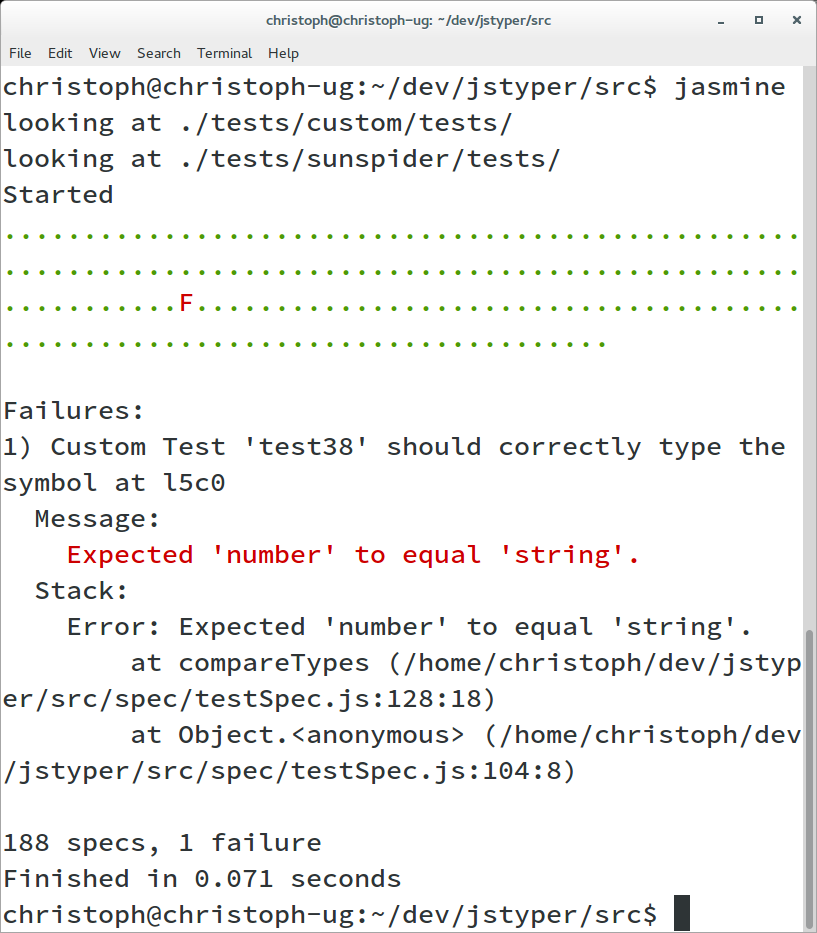
\includegraphics[width=75mm]{../res/jasmine-fail.png}
}
\subfloat[An example test]{
  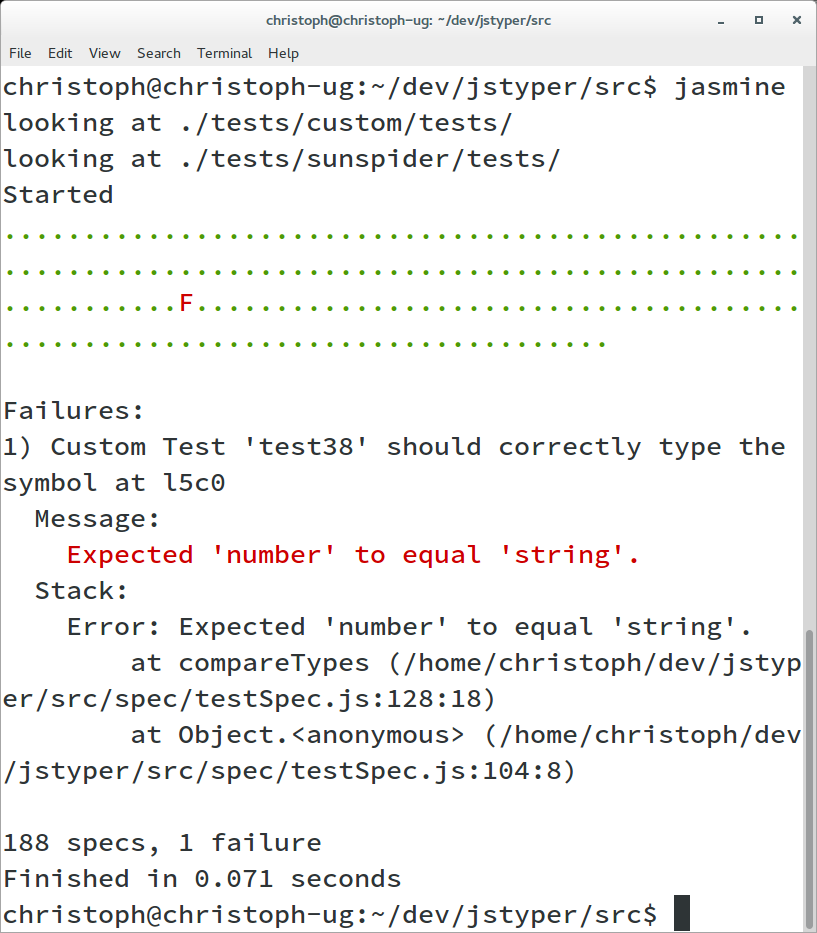
\includegraphics[width=75mm]{../res/jasmine-fail.png}
}

\hspace{0mm}

\newsavebox{\inputbox}
\begin{lrbox}{\inputbox}
\begin{minipage}{75mm}
  \begin{minted}[]{javascript}
  // jstyper start
  // jstyper import x

  var y = x.f();
  y += 5;

  // jstyper end
  \end{minted}
\end{minipage}
\end{lrbox}
\subfloat[An example input]{
  \usebox{\inputbox}
}
\newsavebox{\outputbox}
\begin{lrbox}{\outputbox}
\begin{minipage}{75mm}
  \begin{minted}[]{javascript}
  // jstyper import x
  // y: number
  var y = mimic({
      kind: "object",
      memberTypes: {
          f: {
              kind: "function",
              argTypes: [ {
                  kind: "abstract"
              } ],
              returnType: {
                  kind: "primitive",
                  type: "number"
              }
          }
      }
  }, x).f();

  // y: number
  y += 5;
\end{minted}
\end{minipage}
\end{lrbox}
\subfloat[An example output]{
  \usebox{\outputbox}
}
\caption{Demonstration of the testing procedure}
\end{figure}

\end{document}

\section{Testing and Profiling the Compiler}
\subsection*{Correctness}
\subsection*{Performance}

\chapter{Conclusions}
\section{Future work}
Prototypal Inheritance, Strings as objects \\
Union types, with discharge under type-checks
Auto-detect imported vars by scope analysis \\
Fine-grained object modification by control flow analysis

\printbibliography{}
\end{document}

%%%%%%%%%%%%%%%%%%%%%%%%%%%%%%%%%%%%%%%%%%%%%%%%%%%%%%%%%%%%%%%%%%%%%
% the bibliography
\addcontentsline{toc}{chapter}{Bibliography}
\printbibliography{}

%%%%%%%%%%%%%%%%%%%%%%%%%%%%%%%%%%%%%%%%%%%%%%%%%%%%%%%%%%%%%%%%%%%%%
% the appendices
\appendix

\chapter{Full Language Specification}

% generated by Ott 0.25 from: ../../src/formal/jstyper.ott
\newcommand{\ottdrule}[4][]{{\displaystyle\frac{\begin{array}{l}#2\end{array}}{#3}\quad\ottdrulename{#4}}}
\newcommand{\ottusedrule}[1]{\[#1\]}
\newcommand{\ottpremise}[1]{ #1 \\}
\newenvironment{ottdefnblock}[3][]{ \framebox{\mbox{#2}} \quad #3 \\[0pt]}{}
\newenvironment{ottfundefnblock}[3][]{ \framebox{\mbox{#2}} \quad #3 \\[0pt]\begin{displaymath}\begin{array}{l}}{\end{array}\end{displaymath}}
\newcommand{\ottfunclause}[2]{ #1 \equiv #2 \\}
\newcommand{\ottnt}[1]{\mathit{#1}}
\newcommand{\ottmv}[1]{\mathit{#1}}
\newcommand{\ottkw}[1]{\mathbf{#1}}
\newcommand{\ottsym}[1]{#1}
\newcommand{\ottcom}[1]{\text{#1}}
\newcommand{\ottdrulename}[1]{\textsc{#1}}
\newcommand{\ottcomplu}[5]{\overline{#1}^{\,#2\in #3 #4 #5}}
\newcommand{\ottcompu}[3]{\overline{#1}^{\,#2<#3}}
\newcommand{\ottcomp}[2]{\overline{#1}^{\,#2}}
\newcommand{\ottgrammartabular}[1]{\begin{supertabular}{llcllllll}#1\end{supertabular}}
\newcommand{\ottmetavartabular}[1]{\begin{supertabular}{ll}#1\end{supertabular}}
\newcommand{\ottrulehead}[3]{$#1$ & & $#2$ & & & \multicolumn{2}{l}{#3}}
\newcommand{\ottprodline}[6]{& & $#1$ & $#2$ & $#3 #4$ & $#5$ & $#6$}
\newcommand{\ottfirstprodline}[6]{\ottprodline{#1}{#2}{#3}{#4}{#5}{#6}}
\newcommand{\ottlongprodline}[2]{& & $#1$ & \multicolumn{4}{l}{$#2$}}
\newcommand{\ottfirstlongprodline}[2]{\ottlongprodline{#1}{#2}}
\newcommand{\ottbindspecprodline}[6]{\ottprodline{#1}{#2}{#3}{#4}{#5}{#6}}
\newcommand{\ottprodnewline}{\\}
\newcommand{\ottinterrule}{\\[5.0mm]}
\newcommand{\ottafterlastrule}{\\}

\newcommand{\ottmetavars}{
\ottmetavartabular{
 $ \ottmv{termvar} ,\, \ottmv{x} ,\, \ottmv{y} ,\, \ottmv{z} ,\, \ottmv{id} ,\, \ottmv{l} ,\, \ottmv{this} ,\, \ottmv{return} $ &  \\
 $ \ottmv{index} ,\, \ottmv{i} ,\, \ottmv{j} ,\, \ottmv{k} ,\, \ottmv{o} $ &  \\
}}

\newcommand{\ottv}{
\ottrulehead{\ottnt{v}}{::=}{\ottcom{Values}}\ottprodnewline
\ottfirstprodline{|}{\ottnt{b}}{}{}{}{\ottcom{Boolean}}\ottprodnewline
\ottprodline{|}{\ottnt{n}}{}{}{}{\ottcom{Number}}\ottprodnewline
\ottprodline{|}{\ottkw{str}}{}{}{}{\ottcom{String}}\ottprodnewline
\ottprodline{|}{\ottkw{undefined}}{}{}{}{\ottcom{Undefined}}\ottprodnewline
\ottprodline{|}{\ottkw{null}}{}{}{}{\ottcom{null}}\ottprodnewline
\ottprodline{|}{\ottnt{obj}}{}{}{}{\ottcom{ObjVal}}\ottprodnewline
\ottprodline{|}{\ottnt{arr}}{}{}{}{\ottcom{ArrVal}}\ottprodnewline
\ottprodline{|}{ [\![  \ottnt{func} ,  \ottnt{s}  ]\!] }{}{}{}{\ottcom{FuncClosure}}\ottprodnewline
\ottprodline{|}{\Theta  \ottsym{(}  \ottnt{a}  \ottsym{)}}{}{}{}{\ottcom{GetStore}}\ottprodnewline
\ottprodline{|}{ \ottnt{v_{{\mathrm{1}}}}  \cup  \ottnt{v_{{\mathrm{2}}}} }{}{}{}{\ottcom{ObjUnion}}}

\newcommand{\ottobj}{
\ottrulehead{\ottnt{obj}}{::=}{}\ottprodnewline
\ottfirstprodline{|}{\ottsym{\{}  \ottmv{l_{{\mathrm{1}}}}  \ottsym{:}  \ottnt{v_{{\mathrm{1}}}}  \ottsym{,} \, .. \, \ottsym{,}  \ottmv{l_{\ottmv{i}}}  \ottsym{:}  \ottnt{v_{\ottmv{i}}}  \ottsym{\}}}{}{}{}{\ottcom{ObjVal}}}

\newcommand{\ottarr}{
\ottrulehead{\ottnt{arr}}{::=}{}\ottprodnewline
\ottfirstprodline{|}{\ottsym{[}  \ottnt{v_{{\mathrm{1}}}}  \ottsym{,} \, .. \, \ottsym{,}  \ottnt{v_{{\mathrm{2}}}}  \ottsym{]}}{}{}{}{\ottcom{ArrayVal}}}

\newcommand{\ottfunc}{
\ottrulehead{\ottnt{func}}{::=}{}\ottprodnewline
\ottfirstprodline{|}{\ottkw{function} \, \ottmv{id}  \ottsym{(}  \ottmv{x_{{\mathrm{1}}}}  \ottsym{,} \, .. \, \ottsym{,}  \ottmv{x_{\ottmv{k}}}  \ottsym{)}  \ottsym{\{}  \ottnt{m}  \ottsym{\}}}{}{}{}{\ottcom{FuncVal}}\ottprodnewline
\ottprodline{|}{\ottkw{function} \, \ottsym{(}  \ottmv{x_{{\mathrm{1}}}}  \ottsym{,} \, .. \, \ottsym{,}  \ottmv{x_{\ottmv{k}}}  \ottsym{)}  \ottsym{\{}  \ottnt{m}  \ottsym{\}}}{}{}{}{\ottcom{AnonFuncVal}}}

\newcommand{\otte}{
\ottrulehead{\ottnt{e}}{::=}{\ottcom{Expression}}\ottprodnewline
\ottfirstprodline{|}{\ottnt{v}}{}{}{}{\ottcom{Value}}\ottprodnewline
\ottprodline{|}{\ottmv{id}}{}{}{}{\ottcom{Deref}}\ottprodnewline
\ottprodline{|}{\ottnt{assignTarget} \, \approx \, \ottnt{e_{{\mathrm{2}}}}}{}{}{}{\ottcom{Assign}}\ottprodnewline
\ottprodline{|}{\ottnt{e} \, \ottnt{op} \, \ottnt{e'}}{}{}{}{\ottcom{BinExp}}\ottprodnewline
\ottprodline{|}{\ottnt{assignTarget} \, \ottnt{postAssign}}{}{}{}{\ottcom{PostAssign}}\ottprodnewline
\ottprodline{|}{\ottnt{preAssign} \, \ottnt{assignTarget}}{}{}{}{\ottcom{PreAssign}}\ottprodnewline
\ottprodline{|}{\ottnt{preOp} \, \ottnt{e}}{}{}{}{\ottcom{PreExp}}\ottprodnewline
\ottprodline{|}{\ottsym{\{}  \ottmv{l_{{\mathrm{1}}}}  \ottsym{:}  \ottnt{e_{{\mathrm{1}}}}  \ottsym{,} \, .. \, \ottsym{,}  \ottmv{l_{\ottmv{i}}}  \ottsym{:}  \ottnt{e_{\ottmv{i}}}  \ottsym{\}}}{}{}{}{\ottcom{ObjExp}}\ottprodnewline
\ottprodline{|}{\ottnt{e}  \ottsym{.}  \ottmv{l}}{}{}{}{\ottcom{PropExp}}\ottprodnewline
\ottprodline{|}{\ottnt{e}  \ottsym{[}  \ottnt{e_{{\mathrm{1}}}}  \ottsym{]}}{}{}{}{\ottcom{ArrExp}}\ottprodnewline
\ottprodline{|}{\ottnt{e}  \ottsym{(}  \ottnt{e_{{\mathrm{1}}}}  \ottsym{,} \, .. \, \ottsym{,}  \ottnt{e_{{\mathrm{2}}}}  \ottsym{)}}{}{}{}{\ottcom{CallExp}}\ottprodnewline
\ottprodline{|}{\ottsym{[}  \ottnt{e_{{\mathrm{1}}}}  \ottsym{,} \, .. \, \ottsym{,}  \ottnt{e_{{\mathrm{2}}}}  \ottsym{]}}{}{}{}{\ottcom{ArrayExp}}\ottprodnewline
\ottprodline{|}{\ottnt{assignTarget}}{}{}{}{}\ottprodnewline
\ottprodline{|}{\ottnt{func}}{}{}{}{}\ottprodnewline
\ottprodline{|}{ [\![ @body\{ \ottnt{m} \},  \ottnt{s} ,  \Theta  ]\!] }{}{}{}{}}

\newcommand{\ottAss}{
\ottrulehead{\approx}{::=}{\ottcom{Assignments}}\ottprodnewline
\ottfirstprodline{|}{\ottsym{=}}{}{}{}{\ottcom{PlainAssign}}\ottprodnewline
\ottprodline{|}{\ottnt{numOp}  \ottsym{=}}{}{}{}{\ottcom{NumAssign}}}

\newcommand{\ottvRef}{
\ottrulehead{\ottnt{vRef}}{::=}{}\ottprodnewline
\ottfirstprodline{|}{\ottmv{id}}{}{}{}{}\ottprodnewline
\ottprodline{|}{\ottnt{vRef}  \ottsym{.}  \ottmv{l}}{}{}{}{}\ottprodnewline
\ottprodline{|}{\ottnt{vRef}  \ottsym{[}  \ottnt{n}  \ottsym{]}}{}{}{}{}}

\newcommand{\ottassignTarget}{
\ottrulehead{\ottnt{assignTarget}}{::=}{\ottcom{Assignment Targets}}\ottprodnewline
\ottfirstprodline{|}{\ottnt{vRef}}{}{}{}{}\ottprodnewline
\ottprodline{|}{\ottnt{assignTarget}  \ottsym{[}  \ottnt{e}  \ottsym{]}}{}{}{}{}\ottprodnewline
\ottprodline{|}{\ottnt{assignTarget}  \ottsym{.}  \ottmv{l}}{}{}{}{}}

\newcommand{\ottm}{
\ottrulehead{\ottnt{m}}{::=}{\ottcom{Statement}}\ottprodnewline
\ottfirstprodline{|}{\ottnt{e}}{}{}{}{\ottcom{Expression}}\ottprodnewline
\ottprodline{|}{\ottnt{m_{{\mathrm{1}}}}  \ottsym{;} \, .. \, \ottsym{;}  \ottnt{m_{\ottmv{i}}}}{}{}{}{\ottcom{Seqs}}\ottprodnewline
\ottprodline{|}{\ottnt{varDec}}{}{}{}{\ottcom{VarDeclaration}}\ottprodnewline
\ottprodline{|}{\ottkw{if} \, \ottsym{(}  \ottnt{e}  \ottsym{)}  \ottsym{\{}  \ottnt{m_{{\mathrm{1}}}}  \ottsym{\}}}{}{}{}{\ottcom{IfStatement}}\ottprodnewline
\ottprodline{|}{\ottkw{if} \, \ottsym{(}  \ottnt{e}  \ottsym{)}  \ottsym{\{}  \ottnt{m_{{\mathrm{1}}}}  \ottsym{\}} \, \ottkw{else} \, \ottsym{\{}  \ottnt{m_{{\mathrm{2}}}}  \ottsym{\}}}{}{}{}{\ottcom{IfElseStatement}}\ottprodnewline
\ottprodline{|}{\ottmv{return} \, \ottnt{e}}{}{}{}{\ottcom{ReturnStatement}}\ottprodnewline
\ottprodline{|}{\ottmv{return}}{}{}{}{\ottcom{Return}}\ottprodnewline
\ottprodline{|}{\ottsym{@def} \, \ottkw{function} \, \ottmv{id}  \ottsym{(}  \ottmv{x_{{\mathrm{1}}}}  \ottsym{,} \, .. \, \ottsym{,}  \ottmv{x_{\ottmv{k}}}  \ottsym{)}  \ottsym{\{}  \ottnt{m}  \ottsym{\}}}{}{}{}{\ottcom{FuncDef}}\ottprodnewline
\ottprodline{|}{\ottkw{while} \, \ottsym{(}  \ottnt{e}  \ottsym{)}  \ottsym{\{}  \ottnt{m_{{\mathrm{1}}}}  \ottsym{\}}}{}{}{}{\ottcom{WhileStatement}}\ottprodnewline
\ottprodline{|}{\ottkw{for} \, \ottsym{(}  \ottnt{e_{{\mathrm{1}}}}  \ottsym{;}  \ottnt{e_{{\mathrm{2}}}}  \ottsym{;}  \ottnt{e_{{\mathrm{3}}}}  \ottsym{)}  \ottsym{\{}  \ottnt{m_{{\mathrm{1}}}}  \ottsym{\}}}{}{}{}{\ottcom{ForStatement1}}\ottprodnewline
\ottprodline{|}{\ottkw{for} \, \ottsym{(}  \ottnt{varDec}  \ottsym{;}  \ottnt{e_{{\mathrm{2}}}}  \ottsym{;}  \ottnt{e_{{\mathrm{3}}}}  \ottsym{)}  \ottsym{\{}  \ottnt{m_{{\mathrm{1}}}}  \ottsym{\}}}{}{}{}{\ottcom{ForStatement2}}\ottprodnewline
\ottprodline{|}{ \epsilon }{}{}{}{\ottcom{EmptyStatement}}}

\newcommand{\ottvd}{
\ottrulehead{\ottnt{vd}}{::=}{\ottcom{VariableDeclaration}}\ottprodnewline
\ottfirstprodline{|}{\ottmv{id}}{}{}{}{\ottcom{Declaration}}\ottprodnewline
\ottprodline{|}{\ottmv{id}  \ottsym{=}  \ottnt{e}}{}{}{}{\ottcom{Definition}}}

\newcommand{\ottvarDec}{
\ottrulehead{\ottnt{varDec}}{::=}{}\ottprodnewline
\ottfirstprodline{|}{\ottkw{var} \, \ottnt{vd_{{\mathrm{1}}}}  \ottsym{,} \, ... \, \ottsym{,}  \ottnt{vd_{\ottmv{k}}}}{}{}{}{\ottcom{VarDeclaration}}}

\newcommand{\ottret}{
\ottrulehead{\ottnt{ret}}{::=}{}\ottprodnewline
\ottfirstprodline{|}{\ottmv{return} \, \ottnt{e}}{}{}{}{\ottcom{ReturnExp}}\ottprodnewline
\ottprodline{|}{\ottmv{return}}{}{}{}{\ottcom{Return}}}

\newcommand{\ottop}{
\ottrulehead{\ottnt{op}}{::=}{\ottcom{BinaryOperation}}\ottprodnewline
\ottfirstprodline{|}{\ottnt{numOp}}{}{}{}{\ottcom{NumOp}}\ottprodnewline
\ottprodline{|}{\ottnt{cmpOp}}{}{}{}{\ottcom{CmpOp}}\ottprodnewline
\ottprodline{|}{\ottnt{numcmpOp}}{}{}{}{\ottcom{NumCmpOp}}\ottprodnewline
\ottprodline{|}{\ottnt{boolOp}}{}{}{}{\ottcom{BoolOp}}}

\newcommand{\ottnumOp}{
\ottrulehead{\ottnt{numOp}}{::=}{}\ottprodnewline
\ottfirstprodline{|}{\ottsym{+}}{}{}{}{\ottcom{Addition}}\ottprodnewline
\ottprodline{|}{\ottsym{-}}{}{}{}{\ottcom{Subtraction}}\ottprodnewline
\ottprodline{|}{\ottsym{/}}{}{}{}{\ottcom{Division}}\ottprodnewline
\ottprodline{|}{\ottsym{*}}{}{}{}{\ottcom{Multiplication}}\ottprodnewline
\ottprodline{|}{\ottsym{\%}}{}{}{}{\ottcom{Modulo}}}

\newcommand{\ottnumcmpOp}{
\ottrulehead{\ottnt{numcmpOp}}{::=}{}\ottprodnewline
\ottfirstprodline{|}{\ottsym{<}}{}{}{}{\ottcom{LessThan}}\ottprodnewline
\ottprodline{|}{\ottsym{>}}{}{}{}{\ottcom{GreaterThan}}\ottprodnewline
\ottprodline{|}{ \leq }{}{}{}{\ottcom{LessEqual}}\ottprodnewline
\ottprodline{|}{ \geq }{}{}{}{\ottcom{GreaterEqual}}}

\newcommand{\ottcmpOp}{
\ottrulehead{\ottnt{cmpOp}}{::=}{}\ottprodnewline
\ottfirstprodline{|}{\ottsym{==}}{}{}{}{\ottcom{Equal}}\ottprodnewline
\ottprodline{|}{ !\!\!= }{}{}{}{\ottcom{Unequal}}\ottprodnewline
\ottprodline{|}{\ottsym{===}}{}{}{}{\ottcom{StrictEqual}}\ottprodnewline
\ottprodline{|}{ !\!\!== }{}{}{}{\ottcom{StrictUnequal}}}

\newcommand{\ottboolOp}{
\ottrulehead{\ottnt{boolOp}}{::=}{}\ottprodnewline
\ottfirstprodline{|}{\ottsym{\mbox{$\mid$}\mbox{$\mid$}}}{}{}{}{\ottcom{BooleanOr}}\ottprodnewline
\ottprodline{|}{\ottsym{\&\&}}{}{}{}{\ottcom{BooleanAnd}}}

\newcommand{\ottpreOp}{
\ottrulehead{\ottnt{preOp}}{::=}{\ottcom{PrefixOperation}}\ottprodnewline
\ottfirstprodline{|}{ -\! }{}{}{}{\ottcom{Negation}}\ottprodnewline
\ottprodline{|}{ !\! }{}{}{}{\ottcom{BoolNegation}}}

\newcommand{\ottpreAssign}{
\ottrulehead{\ottnt{preAssign}}{::=}{\ottcom{PreAssign}}\ottprodnewline
\ottfirstprodline{|}{ -\!\!-\!\! }{}{}{}{\ottcom{PreDecrement}}\ottprodnewline
\ottprodline{|}{ +\!\!+\!\! }{}{}{}{\ottcom{PreIncrement}}}

\newcommand{\ottpostAssign}{
\ottrulehead{\ottnt{postAssign}}{::=}{\ottcom{PostAssign}}\ottprodnewline
\ottfirstprodline{|}{ \!\!\!-\!\!- }{}{}{}{\ottcom{PostDecrement}}\ottprodnewline
\ottprodline{|}{ \!\!+\!\!+ }{}{}{}{\ottcom{PostIncrement}}}

\newcommand{\otta}{
\ottrulehead{\ottnt{a}}{::=}{\ottcom{Heap Addresses}}\ottprodnewline
\ottfirstprodline{|}{\ottnt{s}  \ottsym{(}  \ottmv{id}  \ottsym{)}}{}{}{}{\ottcom{StoreAddress}}\ottprodnewline
\ottprodline{|}{\ottnt{a}  \ottsym{[}  \ottmv{l}  \ottsym{]}}{}{}{}{\ottcom{PropAddress}}\ottprodnewline
\ottprodline{|}{\ottnt{a}  \ottsym{[}  \ottnt{n}  \ottsym{]}}{}{}{}{\ottcom{ArrAddress}}\ottprodnewline
\ottprodline{|}{\ottkw{addr} \, \ottsym{(}  \ottnt{e}  \ottsym{,}  \ottnt{s}  \ottsym{,}  \Theta  \ottsym{)}}{}{}{}{\ottcom{AddrLookup}}}

\newcommand{\otts}{
\ottrulehead{\ottnt{s}}{::=}{\ottcom{Store}}\ottprodnewline
\ottfirstprodline{|}{ \ottnt{s_{{\mathrm{1}}}}  \cup  \ottnt{s_{{\mathrm{2}}}} }{}{}{}{\ottcom{StoreUnion}}\ottprodnewline
\ottprodline{|}{\ottsym{\{}  \ottmv{id_{{\mathrm{1}}}}  \ottsym{:}  \ottnt{a_{{\mathrm{1}}}}  \ottsym{,} \, .. \, \ottsym{,}  \ottmv{id_{\ottmv{i}}}  \ottsym{:}  \ottnt{a_{\ottmv{i}}}  \ottsym{\}}}{}{}{}{\ottcom{LiteralStore}}}

\newcommand{\otth}{
\ottrulehead{\Theta}{::=}{\ottcom{Heap}}\ottprodnewline
\ottfirstprodline{|}{ \Theta_{{\mathrm{1}}}  \oplus  \Theta_{{\mathrm{2}}} }{}{}{}{\ottcom{HeapUnion}}\ottprodnewline
\ottprodline{|}{\ottsym{\{}  \ottnt{a_{{\mathrm{1}}}}  \ottsym{:}  \ottnt{v_{{\mathrm{1}}}}  \ottsym{,} \, .. \, \ottsym{,}  \ottnt{a_{\ottmv{k}}}  \ottsym{:}  \ottnt{v_{\ottmv{k}}}  \ottsym{\}}}{}{}{}{\ottcom{LiteralHeap}}}

\newcommand{\ottb}{
\ottrulehead{\ottnt{b}}{::=}{}\ottprodnewline
\ottfirstprodline{|}{\ottkw{true}}{}{}{}{}\ottprodnewline
\ottprodline{|}{\ottkw{false}}{}{}{}{}}

\newcommand{\ottT}{
\ottrulehead{\ottnt{T}}{::=}{\ottcom{Value Type}}\ottprodnewline
\ottfirstprodline{|}{\ottkw{number}}{}{}{}{\ottcom{Number}}\ottprodnewline
\ottprodline{|}{\ottkw{boolean}}{}{}{}{\ottcom{Boolean}}\ottprodnewline
\ottprodline{|}{\ottkw{string}}{}{}{}{\ottcom{String}}\ottprodnewline
\ottprodline{|}{\ottkw{undefined}}{}{}{}{\ottcom{undefined}}\ottprodnewline
\ottprodline{|}{\ottkw{null}}{}{}{}{\ottcom{null}}\ottprodnewline
\ottprodline{|}{\ottsym{\{}  \ottmv{l_{{\mathrm{1}}}}  \ottsym{:}  \ottnt{T_{{\mathrm{1}}}}  \ottsym{,} \, .. \, \ottsym{,}  \ottmv{l_{\ottmv{i}}}  \ottsym{:}  \ottnt{T_{\ottmv{i}}}  \ottsym{\}}}{}{}{}{\ottcom{ObjType}}\ottprodnewline
\ottprodline{|}{\ottnt{T_{{\mathrm{1}}}}  \ottsym{,} \, ... \, \ottsym{,}  \ottnt{T_{\ottmv{i}}}  \rightarrow  \ottnt{T_{\ottmv{j}}}}{}{}{}{\ottcom{FunctionType}}\ottprodnewline
\ottprodline{|}{ [\![  \ottnt{T} ,  \Gamma , ]\!] }{}{}{}{\ottcom{ClosureType}}\ottprodnewline
\ottprodline{|}{\ottsym{[}  \ottnt{T_{{\mathrm{1}}}}  \ottsym{]}}{}{}{}{\ottcom{ArrayType}}\ottprodnewline
\ottprodline{|}{\Gamma  \ottsym{["return"]}}{}{}{}{\ottcom{GammaType}}\ottprodnewline
\ottprodline{|}{\ottkw{IllDefined} \, \ottsym{(}  \ottnt{T}  \ottsym{)}} {\textsf{M}}{}{}{\ottcom{IllDefinedType}}\ottprodnewline
\ottprodline{|}{\ottkw{pending}} {\textsf{M}}{}{}{\ottcom{Pending}}\ottprodnewline
\ottprodline{|}{\ottnt{T_{{\mathrm{1}}}}  \multimapinv  \ottnt{T_{{\mathrm{2}}}}}{}{}{}{\ottcom{DerivedType}}}

\newcommand{\ottG}{
\ottrulehead{\Gamma  ,\ \gamma}{::=}{\ottcom{Context}}\ottprodnewline
\ottfirstprodline{|}{\varnothing}{}{}{}{\ottcom{EmptyContext}}\ottprodnewline
\ottprodline{|}{\ottsym{\{}  \Gamma  \ottsym{\}}}{}{}{}{\ottcom{SingletonContext}}\ottprodnewline
\ottprodline{|}{ \Gamma  \cup  \Gamma' }{}{}{}{\ottcom{UnionContext}}\ottprodnewline
\ottprodline{|}{\ottmv{id}  \ottsym{:}  \ottnt{T}}{}{}{}{\ottcom{ContextItem}}\ottprodnewline
\ottprodline{|}{\ottsym{\{}  \ottmv{id_{{\mathrm{1}}}}  \ottsym{:}  \ottnt{T_{{\mathrm{1}}}}  \ottsym{,} \, .. \, \ottsym{,}  \ottmv{id_{\ottmv{k}}}  \ottsym{:}  \ottnt{T_{\ottmv{k}}}  \ottsym{\}}}{}{}{}{\ottcom{ContextItems}}\ottprodnewline
\ottprodline{|}{\ottsym{merge(}  \Gamma_{{\mathrm{1}}}  \ottsym{,}  \Gamma_{{\mathrm{2}}}  \ottsym{,}  \Gamma_{{\mathrm{3}}}  \ottsym{)}} {\textsf{M}}{}{}{\ottcom{MergedContext}}}

\newcommand{\ottC}{
\ottrulehead{\ottnt{C}}{::=}{\ottcom{Constraint}}\ottprodnewline
\ottfirstprodline{|}{\varnothing}{}{}{}{\ottcom{EmptyConstraint}}\ottprodnewline
\ottprodline{|}{ \ottnt{C}  \cup  \ottnt{C'} }{}{}{}{\ottcom{UnionConstraint}}\ottprodnewline
\ottprodline{|}{ \ottnt{C}  \cap  \ottnt{C'} }{}{}{}{\ottcom{IntersectConstraint}}\ottprodnewline
\ottprodline{|}{ \bigcup \limits_{ \ottnt{setIndex} = \ottnt{n_{{\mathrm{1}}}} }^ \ottnt{n_{{\mathrm{2}}}}   \ottnt{C} }{}{}{}{\ottcom{BigUnion}}\ottprodnewline
\ottprodline{|}{\ottsym{\{}  \ottnt{T_{{\mathrm{1}}}} \, \ottnt{const} \, \ottnt{T_{{\mathrm{2}}}}  \ottsym{\}}}{}{}{}{\ottcom{ConstLeq}}\ottprodnewline
\ottprodline{|}{ \ottnt{C} }{}{}{}{\ottcom{BracketedConstraint}}}

\newcommand{\ottconst}{
\ottrulehead{\ottnt{const}}{::=}{}\ottprodnewline
\ottfirstprodline{|}{ \preceq }{}{}{}{\ottcom{LEqConstraint}}\ottprodnewline
\ottprodline{|}{ \succeq }{}{}{}{\ottcom{GEqConstraint}}\ottprodnewline
\ottprodline{|}{ \preceq_c }{}{}{}{\ottcom{LEqCheckConstraint}}\ottprodnewline
\ottprodline{|}{ \succeq_c }{}{}{}{\ottcom{GEqCheckConstraint}}\ottprodnewline
\ottprodline{|}{ \preceq_o }{}{}{}{\ottcom{LEqOptConstraint}}\ottprodnewline
\ottprodline{|}{ \succeq_o }{}{}{}{\ottcom{GEqOptConstraint}}\ottprodnewline
\ottprodline{|}{ = }{}{}{}{\ottcom{EqConstraint}}}

\newcommand{\ottterminals}{
\ottrulehead{\ottnt{terminals}}{::=}{}\ottprodnewline
\ottfirstprodline{|}{ \rightarrow }{}{}{}{}\ottprodnewline
\ottprodline{|}{ \multimapinv }{}{}{}{}\ottprodnewline
\ottprodline{|}{ \vdash }{}{}{}{}\ottprodnewline
\ottprodline{|}{\ottsym{;}}{}{}{}{}\ottprodnewline
\ottprodline{|}{\ottkw{var}}{}{}{}{}\ottprodnewline
\ottprodline{|}{ \varnothing }{}{}{}{}}

\newcommand{\ottmaps}{
\ottrulehead{\ottnt{maps}}{::=}{}\ottprodnewline
\ottfirstprodline{|}{\Gamma}{}{}{}{}\ottprodnewline
\ottprodline{|}{\Theta}{}{}{}{}\ottprodnewline
\ottprodline{|}{\ottnt{s}}{}{}{}{}\ottprodnewline
\ottprodline{|}{\ottkw{addr}}{}{}{}{}}

\newcommand{\ottsv}{
\ottrulehead{\ottnt{sv}}{::=}{\ottcom{SetVar}}\ottprodnewline
\ottfirstprodline{|}{\ottnt{C}}{}{}{}{\ottcom{ConstraintSet}}\ottprodnewline
\ottprodline{|}{\ottkw{X}}{}{}{}{\ottcom{VariableSet}}\ottprodnewline
\ottprodline{|}{\ottsym{dom(}  \ottnt{maps}  \ottsym{)}}{}{}{}{}\ottprodnewline
\ottprodline{|}{\ottsym{codom(}  \ottnt{maps}  \ottsym{)}}{}{}{}{}}

\newcommand{\ottfv}{
\ottrulehead{\ottnt{fv}}{::=}{\ottcom{FormulaVar}}\ottprodnewline
\ottfirstprodline{|}{\Gamma}{}{}{}{\ottcom{ContextVar}}\ottprodnewline
\ottprodline{|}{\Gamma  \ottsym{(}  \ottmv{id}  \ottsym{)}}{}{}{}{\ottcom{ContextMember}}\ottprodnewline
\ottprodline{|}{\ottnt{sv}}{}{}{}{\ottcom{SetFormulaVar}}\ottprodnewline
\ottprodline{|}{\ottnt{T}}{}{}{}{\ottcom{TypeFormulaVar}}\ottprodnewline
\ottprodline{|}{\ottmv{id}}{}{}{}{\ottcom{IDFormulaVar}}\ottprodnewline
\ottprodline{|}{\ottnt{func}}{}{}{}{\ottcom{FuncFormulaVar}}\ottprodnewline
\ottprodline{|}{\ottnt{m}}{}{}{}{\ottcom{ExpFormulaVar}}\ottprodnewline
\ottprodline{|}{\ottnt{a}}{}{}{}{}\ottprodnewline
\ottprodline{|}{\ottnt{maps}}{}{}{}{}\ottprodnewline
\ottprodline{|}{\ottsym{(}  \ottnt{fv_{{\mathrm{1}}}}  \ottsym{,} \, .. \, \ottsym{,}  \ottnt{fv_{\ottmv{i}}}  \ottsym{)}}{}{}{}{}}

\newcommand{\ottn}{
\ottrulehead{\ottnt{n}}{::=}{}\ottprodnewline
\ottfirstprodline{|}{\ottsym{0}}{}{}{}{}\ottprodnewline
\ottprodline{|}{\ottsym{1}}{}{}{}{}\ottprodnewline
\ottprodline{|}{\ottsym{2}}{}{}{}{}\ottprodnewline
\ottprodline{|}{\ottsym{3}}{}{}{}{}\ottprodnewline
\ottprodline{|}{\ottnt{setIndex}}{}{}{}{}}

\newcommand{\ottsetIndex}{
\ottrulehead{\ottnt{setIndex}}{::=}{}\ottprodnewline
\ottfirstprodline{|}{\ottmv{i}}{}{}{}{}\ottprodnewline
\ottprodline{|}{\ottmv{k}}{}{}{}{}\ottprodnewline
\ottprodline{|}{\ottmv{j}}{}{}{}{}}

\newcommand{\ottformula}{
\ottrulehead{\ottnt{formula}}{::=}{}\ottprodnewline
\ottfirstprodline{|}{\ottnt{judgement}}{}{}{}{\ottcom{judgement}}\ottprodnewline
\ottprodline{|}{ \neg  \ottnt{formula} }{}{}{}{\ottcom{not}}\ottprodnewline
\ottprodline{|}{ ( \ottnt{formula} \!) }{}{}{}{\ottcom{brackets}}\ottprodnewline
\ottprodline{|}{ \ottnt{formula} }{}{}{}{\ottcom{bracketsHidden}}\ottprodnewline
\ottprodline{|}{ \ottnt{formula_{{\mathrm{1}}}}  \quad\hdots\quad  \ottnt{formula_{\ottmv{k}}} }{}{}{}{\ottcom{listForm}}\ottprodnewline
\ottprodline{|}{ \ottnt{formula}  \vee  \ottsym{formula’} }{}{}{}{\ottcom{or}}\ottprodnewline
\ottprodline{|}{ \ottnt{formula}  \wedge  \ottsym{formula’} }{}{}{}{\ottcom{and}}\ottprodnewline
\ottprodline{|}{ \ottnt{formula}  \hspace{1pc}\textit{for}\hspace{6pt}  \ottnt{formula'} }{}{}{}{\ottcom{condform}}\ottprodnewline
\ottprodline{|}{ \forall  \ottnt{setIndex} \ottnt{formula} }{}{}{}{\ottcom{ForAll}}\ottprodnewline
\ottprodline{|}{ \forall  \ottnt{setIndex} \in \ottnt{sv} \ottnt{formula} }{}{}{}{\ottcom{ForAllIn}}\ottprodnewline
\ottprodline{|}{\ottnt{fv}  \ottsym{=}  \ottnt{fv_{{\mathrm{2}}}}}{}{}{}{\ottcom{fequal}}\ottprodnewline
\ottprodline{|}{ \ottnt{fv}  \neq  \ottnt{fv_{{\mathrm{2}}}} }{}{}{}{\ottcom{fnotequal}}\ottprodnewline
\ottprodline{|}{ \ottnt{fv}  \in  \ottnt{sv_{{\mathrm{2}}}} }{}{}{}{\ottcom{Contains}}\ottprodnewline
\ottprodline{|}{ \ottnt{fv}  \notin  \ottnt{sv_{{\mathrm{2}}}} }{}{}{}{\ottcom{NotContains}}\ottprodnewline
\ottprodline{|}{\ottnt{T} \, \ottkw{is} \, \ottkw{fresh}}{}{}{}{\ottcom{Fresh}}\ottprodnewline
\ottprodline{|}{\ottnt{T_{{\mathrm{1}}}}  \ottsym{,} \, .. \, \ottsym{,}  \ottnt{T_{\ottmv{i}}} \, \ottkw{are} \, \ottkw{fresh}}{}{}{}{\ottcom{Freshs}}\ottprodnewline
\ottprodline{|}{\ottnt{a} \, \ottkw{is} \, \ottkw{fresh}}{}{}{}{\ottcom{FreshAddress}}\ottprodnewline
\ottprodline{|}{\ottsym{a1,}  \ottsym{..,}  \ottnt{a_{\ottmv{k}}} \, \ottkw{are} \, \ottkw{fresh}}{}{}{}{\ottcom{FreshAddresses}}\ottprodnewline
\ottprodline{|}{ \ottnt{sv_{{\mathrm{1}}}}  \subseteq  \ottnt{sv_{{\mathrm{2}}}} }{}{}{}{\ottcom{Subset}}}

\newcommand{\ottJop}{
\ottrulehead{\ottnt{Jop}}{::=}{}\ottprodnewline
\ottfirstprodline{|}{ \langle  \ottnt{m} ,  \ottnt{s} ,  \Theta  \rangle  \rightarrow  \langle  \ottnt{m'} ,  \ottnt{s'} ,  \Theta'  \rangle }{}{}{}{}\ottprodnewline
\ottprodline{|}{ \Gamma   \vdash   \ottnt{e}  :  \ottnt{T} \hspace{5pt}| _{  \ottnt{C}  } \hspace{5pt}  \Gamma' }{}{}{}{}\ottprodnewline
\ottprodline{|}{ \Gamma   \vdash   \ottnt{m}  \hspace{5pt}| _{  \ottnt{C}  } \hspace{5pt}  \Gamma' }{}{}{}{}\ottprodnewline
\ottprodline{|}{ \Gamma  \vdash (s, \Theta) } {\textsf{M}}{}{}{}}

\newcommand{\ottjudgement}{
\ottrulehead{\ottnt{judgement}}{::=}{}\ottprodnewline
\ottfirstprodline{|}{\ottnt{Jop}}{}{}{}{}}

\newcommand{\ottuserXXsyntax}{
\ottrulehead{\ottnt{user\_syntax}}{::=}{}\ottprodnewline
\ottfirstprodline{|}{\ottmv{termvar}}{}{}{}{}\ottprodnewline
\ottprodline{|}{\ottmv{index}}{}{}{}{}\ottprodnewline
\ottprodline{|}{\ottnt{v}}{}{}{}{}\ottprodnewline
\ottprodline{|}{\ottnt{obj}}{}{}{}{}\ottprodnewline
\ottprodline{|}{\ottnt{arr}}{}{}{}{}\ottprodnewline
\ottprodline{|}{\ottnt{func}}{}{}{}{}\ottprodnewline
\ottprodline{|}{\ottnt{e}}{}{}{}{}\ottprodnewline
\ottprodline{|}{\approx}{}{}{}{}\ottprodnewline
\ottprodline{|}{\ottnt{vRef}}{}{}{}{}\ottprodnewline
\ottprodline{|}{\ottnt{assignTarget}}{}{}{}{}\ottprodnewline
\ottprodline{|}{\ottnt{m}}{}{}{}{}\ottprodnewline
\ottprodline{|}{\ottnt{vd}}{}{}{}{}\ottprodnewline
\ottprodline{|}{\ottnt{varDec}}{}{}{}{}\ottprodnewline
\ottprodline{|}{\ottnt{ret}}{}{}{}{}\ottprodnewline
\ottprodline{|}{\ottnt{op}}{}{}{}{}\ottprodnewline
\ottprodline{|}{\ottnt{numOp}}{}{}{}{}\ottprodnewline
\ottprodline{|}{\ottnt{numcmpOp}}{}{}{}{}\ottprodnewline
\ottprodline{|}{\ottnt{cmpOp}}{}{}{}{}\ottprodnewline
\ottprodline{|}{\ottnt{boolOp}}{}{}{}{}\ottprodnewline
\ottprodline{|}{\ottnt{preOp}}{}{}{}{}\ottprodnewline
\ottprodline{|}{\ottnt{preAssign}}{}{}{}{}\ottprodnewline
\ottprodline{|}{\ottnt{postAssign}}{}{}{}{}\ottprodnewline
\ottprodline{|}{\ottnt{a}}{}{}{}{}\ottprodnewline
\ottprodline{|}{\ottnt{s}}{}{}{}{}\ottprodnewline
\ottprodline{|}{\Theta}{}{}{}{}\ottprodnewline
\ottprodline{|}{\ottnt{b}}{}{}{}{}\ottprodnewline
\ottprodline{|}{\ottnt{T}}{}{}{}{}\ottprodnewline
\ottprodline{|}{\Gamma}{}{}{}{}\ottprodnewline
\ottprodline{|}{\ottnt{C}}{}{}{}{}\ottprodnewline
\ottprodline{|}{\ottnt{const}}{}{}{}{}\ottprodnewline
\ottprodline{|}{\ottnt{terminals}}{}{}{}{}\ottprodnewline
\ottprodline{|}{\ottnt{maps}}{}{}{}{}\ottprodnewline
\ottprodline{|}{\ottnt{sv}}{}{}{}{}\ottprodnewline
\ottprodline{|}{\ottnt{fv}}{}{}{}{}\ottprodnewline
\ottprodline{|}{\ottnt{n}}{}{}{}{}\ottprodnewline
\ottprodline{|}{\ottnt{setIndex}}{}{}{}{}\ottprodnewline
\ottprodline{|}{\ottnt{formula}}{}{}{}{}}

\newcommand{\ottgrammar}{\ottgrammartabular{
\ottv\ottinterrule
\ottobj\ottinterrule
\ottarr\ottinterrule
\ottfunc\ottinterrule
\otte\ottinterrule
\ottAss\ottinterrule
\ottvRef\ottinterrule
\ottassignTarget\ottinterrule
\ottm\ottinterrule
\ottvd\ottinterrule
\ottvarDec\ottinterrule
\ottret\ottinterrule
\ottop\ottinterrule
\ottnumOp\ottinterrule
\ottnumcmpOp\ottinterrule
\ottcmpOp\ottinterrule
\ottboolOp\ottinterrule
\ottpreOp\ottinterrule
\ottpreAssign\ottinterrule
\ottpostAssign\ottinterrule
\ottT\ottinterrule
}}

% defnss
% defns Jop
%% defn reduce
\newcommand{\ottdruleFunc}[1]{\ottdrule[#1]{%
}{
 \langle  \ottnt{func} ,  \ottnt{s} ,  \Theta  \rangle  \rightarrow  \langle   [\![  \ottnt{func} ,  \ottnt{s}  ]\!]  ,  \ottnt{s} ,  \Theta  \rangle }{%
{\ottdrulename{Func}}{}%
}}


\newcommand{\ottdruleObj}[1]{\ottdrule[#1]{%
\ottpremise{ \langle  \ottnt{e} ,  \ottnt{s} ,  \Theta  \rangle  \rightarrow  \langle  \ottnt{e'} ,  \ottnt{s'} ,  \Theta'  \rangle }%
}{
 \langle  \ottsym{\{}  \ottmv{l_{{\mathrm{1}}}}  \ottsym{:}  \ottnt{v_{{\mathrm{1}}}}  \ottsym{,} \, .. \, \ottsym{,}  \ottmv{l_{\ottmv{j}}}  \ottsym{:}  \ottnt{v_{\ottmv{j}}}  \ottsym{,}  \ottmv{l}  \ottsym{:}  \ottnt{e}  \ottsym{,}  \ottmv{l'_{{\mathrm{1}}}}  \ottsym{:}  \ottnt{e_{{\mathrm{1}}}}  \ottsym{,} \, .. \, \ottsym{,}  \ottmv{l'_{\ottmv{j}}}  \ottsym{:}  \ottnt{e_{\ottmv{j}}}  \ottsym{\}} ,  \ottnt{s} ,  \Theta  \rangle  \rightarrow  \langle  \ottsym{\{}  \ottmv{l_{{\mathrm{1}}}}  \ottsym{:}  \ottnt{v_{{\mathrm{1}}}}  \ottsym{,} \, .. \, \ottsym{,}  \ottmv{l_{\ottmv{j}}}  \ottsym{:}  \ottnt{v_{\ottmv{j}}}  \ottsym{,}  \ottmv{l}  \ottsym{:}  \ottnt{e'}  \ottsym{,}  \ottmv{l'_{{\mathrm{1}}}}  \ottsym{:}  \ottnt{e_{{\mathrm{1}}}}  \ottsym{,} \, .. \, \ottsym{,}  \ottmv{l'_{\ottmv{j}}}  \ottsym{:}  \ottnt{e_{\ottmv{j}}}  \ottsym{\}} ,  \ottnt{s'} ,  \Theta  \rangle }{%
{\ottdrulename{Obj}}{}%
}}


\newcommand{\ottdruleArr}[1]{\ottdrule[#1]{%
\ottpremise{ \langle  \ottnt{e} ,  \ottnt{s} ,  \Theta  \rangle  \rightarrow  \langle  \ottnt{e'} ,  \ottnt{s'} ,  \Theta'  \rangle }%
}{
 \langle  \ottsym{[}  \ottnt{v_{{\mathrm{1}}}}  \ottsym{,} \, .. \, \ottsym{,}  \ottnt{v_{\ottmv{j}}}  \ottsym{,}  \ottnt{e}  \ottsym{,}  \ottnt{e_{{\mathrm{1}}}}  \ottsym{,} \, .. \, \ottsym{,}  \ottnt{e_{\ottmv{k}}}  \ottsym{]} ,  \ottnt{s} ,  \Theta  \rangle  \rightarrow  \langle  \ottsym{[}  \ottnt{v_{{\mathrm{1}}}}  \ottsym{,} \, .. \, \ottsym{,}  \ottnt{v_{\ottmv{j}}}  \ottsym{,}  \ottnt{e'}  \ottsym{,}  \ottnt{e_{{\mathrm{1}}}}  \ottsym{,} \, .. \, \ottsym{,}  \ottnt{e_{\ottmv{k}}}  \ottsym{]} ,  \ottnt{s'} ,  \Theta'  \rangle }{%
{\ottdrulename{Arr}}{}%
}}


\newcommand{\ottdruleDeref}[1]{\ottdrule[#1]{%
\ottpremise{ \ottmv{id}  \in  \ottsym{dom(}  \ottnt{s}  \ottsym{)} }%
\ottpremise{ \ottnt{s}  \ottsym{(}  \ottmv{id}  \ottsym{)}  \in  \ottsym{dom(}  \Theta  \ottsym{)} }%
}{
 \langle  \ottmv{id} ,  \ottnt{s} ,  \Theta  \rangle  \rightarrow  \langle  \Theta  \ottsym{(}  \ottnt{s}  \ottsym{(}  \ottmv{id}  \ottsym{)}  \ottsym{)} ,  \ottnt{s} ,  \Theta  \rangle }{%
{\ottdrulename{Deref}}{}%
}}


\newcommand{\ottdrulePropOne}[1]{\ottdrule[#1]{%
\ottpremise{ \ottnt{e}  \neq  \ottnt{vRef} }%
\ottpremise{ \langle  \ottnt{e} ,  \ottnt{s} ,  \Theta  \rangle  \rightarrow  \langle  \ottnt{e'} ,  \ottnt{s'} ,  \Theta'  \rangle }%
}{
 \langle  \ottnt{e}  \ottsym{.}  \ottmv{l} ,  \ottnt{s} ,  \Theta  \rangle  \rightarrow  \langle  \ottnt{e'}  \ottsym{.}  \ottmv{l} ,  \ottnt{s'} ,  \Theta'  \rangle }{%
{\ottdrulename{Prop1}}{}%
}}


\newcommand{\ottdrulePropTwo}[1]{\ottdrule[#1]{%
}{
 \langle  \ottsym{\{}  \ottmv{l_{{\mathrm{1}}}}  \ottsym{:}  \ottnt{v_{{\mathrm{1}}}}  \ottsym{,} \, .. \, \ottsym{,}  \ottmv{l_{\ottmv{j}}}  \ottsym{:}  \ottnt{v_{\ottmv{j}}}  \ottsym{,}  \ottmv{l}  \ottsym{:}  \ottnt{v}  \ottsym{,}  \ottmv{l'_{{\mathrm{1}}}}  \ottsym{:}  \ottnt{v'_{{\mathrm{1}}}}  \ottsym{,} \, .. \, \ottsym{,}  \ottmv{l'_{\ottmv{j}}}  \ottsym{:}  \ottnt{v'_{\ottmv{j}}}  \ottsym{\}}  \ottsym{.}  \ottmv{l} ,  \ottnt{s} ,  \Theta  \rangle  \rightarrow  \langle  \ottnt{v} ,  \ottnt{s'} ,  \Theta'  \rangle }{%
{\ottdrulename{Prop2}}{}%
}}


\newcommand{\ottdruleArrGetOne}[1]{\ottdrule[#1]{%
\ottpremise{ \ottnt{e}  \neq  \ottnt{vRef} }%
\ottpremise{ \langle  \ottnt{e} ,  \ottnt{s} ,  \Theta  \rangle  \rightarrow  \langle  \ottnt{e'} ,  \ottnt{s'} ,  \Theta'  \rangle }%
}{
 \langle  \ottnt{e}  \ottsym{[}  \ottnt{e_{{\mathrm{2}}}}  \ottsym{]} ,  \ottnt{s} ,  \Theta  \rangle  \rightarrow  \langle  \ottnt{e'}  \ottsym{[}  \ottnt{e_{{\mathrm{2}}}}  \ottsym{]} ,  \ottnt{s'} ,  \Theta'  \rangle }{%
{\ottdrulename{ArrGet1}}{}%
}}


\newcommand{\ottdruleArrGetTwo}[1]{\ottdrule[#1]{%
\ottpremise{ \langle  \ottnt{e} ,  \ottnt{s} ,  \Theta  \rangle  \rightarrow  \langle  \ottnt{e'} ,  \ottnt{s'} ,  \Theta'  \rangle }%
}{
 \langle  \ottnt{vRef}  \ottsym{[}  \ottnt{e}  \ottsym{]} ,  \ottnt{s} ,  \Theta  \rangle  \rightarrow  \langle  \ottnt{vRef}  \ottsym{[}  \ottnt{e'}  \ottsym{]} ,  \ottnt{s'} ,  \Theta'  \rangle }{%
{\ottdrulename{ArrGet2}}{}%
}}


\newcommand{\ottdruleArrGetThree}[1]{\ottdrule[#1]{%
}{
 \langle  \ottsym{[}  \ottnt{v_{{\mathrm{1}}}}  \ottsym{,} \, .. \, \ottsym{,}  \ottnt{v_{\ottmv{j}}}  \ottsym{]}  \ottsym{[}  \ottmv{k}  \ottsym{]} ,  \ottnt{s} ,  \Theta  \rangle  \rightarrow  \langle  \ottnt{v_{\ottmv{k}}} ,  \ottnt{s} ,  \Theta  \rangle }{%
{\ottdrulename{ArrGet3}}{}%
}}


\newcommand{\ottdruleVRef}[1]{\ottdrule[#1]{%
\ottpremise{ \ottsym{(}  \ottnt{vRef}  \ottsym{,}  \ottnt{s}  \ottsym{,}  \Theta  \ottsym{)}  \in  \ottsym{dom(}  \ottkw{addr}  \ottsym{)} }%
\ottpremise{\ottnt{v}  \ottsym{=}  \Theta  \ottsym{(}  \ottkw{addr} \, \ottsym{(}  \ottnt{vRef}  \ottsym{,}  \ottnt{s}  \ottsym{,}  \Theta  \ottsym{)}  \ottsym{)}}%
}{
 \langle  \ottnt{vRef} ,  \ottnt{s} ,  \Theta  \rangle  \rightarrow  \langle  \ottnt{v} ,  \ottnt{s'} ,  \Theta'  \rangle }{%
{\ottdrulename{VRef}}{}%
}}


\newcommand{\ottdruleCallOne}[1]{\ottdrule[#1]{%
\ottpremise{ \ottnt{e}  \neq  \ottnt{v}  \ottsym{.}  \ottmv{l} }%
\ottpremise{ \langle  \ottnt{e} ,  \ottnt{s} ,  \Theta  \rangle  \rightarrow  \langle  \ottnt{e'} ,  \ottnt{s'} ,  \Theta'  \rangle }%
}{
 \langle  \ottnt{e}  \ottsym{(}  \ottnt{e_{{\mathrm{1}}}}  \ottsym{,} \, .. \, \ottsym{,}  \ottnt{e_{\ottmv{i}}}  \ottsym{)} ,  \ottnt{s} ,  \Theta  \rangle  \rightarrow  \langle  \ottnt{e'}  \ottsym{(}  \ottnt{e_{{\mathrm{1}}}}  \ottsym{,} \, .. \, \ottsym{,}  \ottnt{e_{\ottmv{i}}}  \ottsym{)} ,  \ottnt{s'} ,  \Theta'  \rangle }{%
{\ottdrulename{Call1}}{}%
}}


\newcommand{\ottdruleCallTwo}[1]{\ottdrule[#1]{%
\ottpremise{ \langle  \ottnt{e_{{\mathrm{1}}}} ,  \ottnt{s} ,  \Theta  \rangle  \rightarrow  \langle  \ottnt{e'_{{\mathrm{1}}}} ,  \ottnt{s'} ,  \Theta'  \rangle }%
}{
 \langle  \ottnt{v}  \ottsym{(}  \ottnt{v_{{\mathrm{1}}}}  \ottsym{,} \, .. \, \ottsym{,}  \ottnt{v_{\ottmv{i}}}  \ottsym{,}  \ottnt{e_{{\mathrm{1}}}}  \ottsym{,}  \ottnt{e_{{\mathrm{2}}}}  \ottsym{,} \, .. \, \ottsym{,}  \ottnt{e_{\ottmv{j}}}  \ottsym{)} ,  \ottnt{s} ,  \Theta  \rangle  \rightarrow  \langle  \ottnt{v}  \ottsym{(}  \ottnt{v_{{\mathrm{1}}}}  \ottsym{,} \, .. \, \ottsym{,}  \ottnt{v_{\ottmv{i}}}  \ottsym{,}  \ottnt{e'_{{\mathrm{1}}}}  \ottsym{,}  \ottnt{e_{{\mathrm{2}}}}  \ottsym{,} \, .. \, \ottsym{,}  \ottnt{e_{\ottmv{j}}}  \ottsym{)} ,  \ottnt{s'} ,  \Theta'  \rangle }{%
{\ottdrulename{Call2}}{}%
}}


\newcommand{\ottdruleCallNamed}[1]{\ottdrule[#1]{%
\ottpremise{\ottnt{a} \, \ottkw{is} \, \ottkw{fresh}}%
\ottpremise{\ottnt{a_{{\mathrm{0}}}} \, \ottkw{is} \, \ottkw{fresh}}%
\ottpremise{\ottsym{a1,}  \ottsym{..,}  \ottnt{a_{\ottmv{i}}} \, \ottkw{are} \, \ottkw{fresh}}%
\ottpremise{\ottnt{s'_{\ottmv{o}}}  \ottsym{=}   \ottnt{s'}  \cup  \ottsym{\{}  \ottmv{id}  \ottsym{:}  \ottnt{a}  \ottsym{,}  \ottmv{this}  \ottsym{:}  \ottnt{a_{{\mathrm{0}}}}  \ottsym{,}  \ottmv{x_{{\mathrm{1}}}}  \ottsym{:}  \ottnt{a_{{\mathrm{1}}}}  \ottsym{,} \, .. \, \ottsym{,}  \ottmv{x_{\ottmv{i}}}  \ottsym{:}  \ottnt{a_{\ottmv{i}}}  \ottsym{\}} }%
\ottpremise{\Theta_{\ottmv{o}}  \ottsym{=}   \Theta  \oplus  \ottsym{\{}  \ottnt{a}  \ottsym{:}   [\![  \ottkw{function} \, \ottmv{id}  \ottsym{(}  \ottmv{x_{{\mathrm{1}}}}  \ottsym{,} \, .. \, \ottsym{,}  \ottmv{x_{\ottmv{i}}}  \ottsym{)}  \ottsym{\{}  \ottnt{m}  \ottsym{\}} ,  \ottnt{s'}  ]\!]   \ottsym{,}  \ottnt{a_{{\mathrm{0}}}}  \ottsym{:}  \ottkw{undefined}  \ottsym{,}  \ottnt{a_{{\mathrm{1}}}}  \ottsym{:}  \ottnt{v_{{\mathrm{1}}}}  \ottsym{,} \, .. \, \ottsym{,}  \ottnt{a_{\ottmv{i}}}  \ottsym{:}  \ottnt{v_{\ottmv{i}}}  \ottsym{\}} }%
}{
 \langle   [\![  \ottkw{function} \, \ottmv{id}  \ottsym{(}  \ottmv{x_{{\mathrm{1}}}}  \ottsym{,} \, .. \, \ottsym{,}  \ottmv{x_{\ottmv{i}}}  \ottsym{)}  \ottsym{\{}  \ottnt{m}  \ottsym{\}} ,  \ottnt{s'}  ]\!]   \ottsym{(}  \ottnt{v_{{\mathrm{1}}}}  \ottsym{,} \, .. \, \ottsym{,}  \ottnt{v_{\ottmv{i}}}  \ottsym{)} ,  \ottnt{s} ,  \Theta  \rangle  \rightarrow  \langle   [\![ @body\{ \ottnt{m} \},  \ottnt{s'_{\ottmv{o}}} ,  \Theta_{\ottmv{o}}  ]\!]  ,  \ottnt{s} ,  \Theta_{\ottmv{o}}  \rangle }{%
{\ottdrulename{CallNamed}}{}%
}}


\newcommand{\ottdruleCallAnon}[1]{\ottdrule[#1]{%
\ottpremise{\ottnt{a_{{\mathrm{0}}}} \, \ottkw{is} \, \ottkw{fresh}}%
\ottpremise{\ottsym{a1,}  \ottsym{..,}  \ottnt{a_{\ottmv{i}}} \, \ottkw{are} \, \ottkw{fresh}}%
\ottpremise{\ottnt{s'_{\ottmv{o}}}  \ottsym{=}   \ottnt{s'}  \cup  \ottsym{\{}  \ottmv{this}  \ottsym{:}  \ottnt{a_{{\mathrm{0}}}}  \ottsym{,}  \ottmv{x_{{\mathrm{1}}}}  \ottsym{:}  \ottnt{a_{{\mathrm{1}}}}  \ottsym{,} \, .. \, \ottsym{,}  \ottmv{x_{\ottmv{i}}}  \ottsym{:}  \ottnt{a_{\ottmv{i}}}  \ottsym{\}} }%
\ottpremise{\Theta_{\ottmv{o}}  \ottsym{=}   \Theta  \oplus  \ottsym{\{}  \ottnt{a_{{\mathrm{0}}}}  \ottsym{:}  \ottkw{undefined}  \ottsym{,}  \ottnt{a_{{\mathrm{1}}}}  \ottsym{:}  \ottnt{v_{{\mathrm{1}}}}  \ottsym{,} \, .. \, \ottsym{,}  \ottnt{a_{\ottmv{i}}}  \ottsym{:}  \ottnt{v_{\ottmv{i}}}  \ottsym{\}} }%
}{
 \langle   [\![  \ottkw{function} \, \ottsym{(}  \ottmv{x_{{\mathrm{1}}}}  \ottsym{,} \, .. \, \ottsym{,}  \ottmv{x_{\ottmv{i}}}  \ottsym{)}  \ottsym{\{}  \ottnt{m}  \ottsym{\}} ,  \ottnt{s'}  ]\!]   \ottsym{(}  \ottnt{v_{{\mathrm{1}}}}  \ottsym{,} \, .. \, \ottsym{,}  \ottnt{v_{\ottmv{i}}}  \ottsym{)} ,  \ottnt{s} ,  \Theta  \rangle  \rightarrow  \langle   [\![ @body\{ \ottnt{m} \},  \ottnt{s'_{\ottmv{o}}} ,  \Theta_{\ottmv{o}}  ]\!]  ,  \ottnt{s} ,  \Theta_{\ottmv{o}}  \rangle }{%
{\ottdrulename{CallAnon}}{}%
}}


\newcommand{\ottdrulePropCallNamed}[1]{\ottdrule[#1]{%
\ottpremise{\ottnt{a} \, \ottkw{is} \, \ottkw{fresh}}%
\ottpremise{\ottnt{a_{{\mathrm{0}}}} \, \ottkw{is} \, \ottkw{fresh}}%
\ottpremise{\ottsym{a1,}  \ottsym{..,}  \ottnt{a_{\ottmv{i}}} \, \ottkw{are} \, \ottkw{fresh}}%
\ottpremise{ \langle  \ottnt{v_{{\mathrm{0}}}}  \ottsym{.}  \ottmv{l} ,  \ottnt{s} ,  \Theta  \rangle  \rightarrow  \langle   [\![  \ottkw{function} \, \ottmv{id}  \ottsym{(}  \ottmv{x_{{\mathrm{1}}}}  \ottsym{,} \, .. \, \ottsym{,}  \ottmv{x_{\ottmv{i}}}  \ottsym{)}  \ottsym{\{}  \ottnt{m}  \ottsym{\}} ,  \ottnt{s'}  ]\!]  ,  \ottnt{s''} ,  \Theta'  \rangle }%
\ottpremise{\ottnt{s'_{\ottmv{o}}}  \ottsym{=}   \ottnt{s'}  \cup  \ottsym{\{}  \ottmv{id}  \ottsym{:}  \ottnt{a}  \ottsym{,}  \ottmv{this}  \ottsym{:}  \ottnt{a_{{\mathrm{0}}}}  \ottsym{,}  \ottmv{x_{{\mathrm{1}}}}  \ottsym{:}  \ottnt{a_{{\mathrm{1}}}}  \ottsym{,} \, .. \, \ottsym{,}  \ottmv{x_{\ottmv{i}}}  \ottsym{:}  \ottnt{a_{\ottmv{i}}}  \ottsym{\}} }%
\ottpremise{\Theta'_{\ottmv{o}}  \ottsym{=}   \Theta'  \oplus  \ottsym{\{}  \ottnt{a}  \ottsym{:}   [\![  \ottkw{function} \, \ottmv{id}  \ottsym{(}  \ottmv{x_{{\mathrm{1}}}}  \ottsym{,} \, .. \, \ottsym{,}  \ottmv{x_{\ottmv{i}}}  \ottsym{)}  \ottsym{\{}  \ottnt{m}  \ottsym{\}} ,  \ottnt{s'}  ]\!]   \ottsym{,}  \ottnt{a_{{\mathrm{0}}}}  \ottsym{:}  \ottnt{v_{{\mathrm{0}}}}  \ottsym{,}  \ottnt{a_{{\mathrm{1}}}}  \ottsym{:}  \ottnt{v_{{\mathrm{1}}}}  \ottsym{,} \, .. \, \ottsym{,}  \ottnt{a_{\ottmv{i}}}  \ottsym{:}  \ottnt{v_{\ottmv{i}}}  \ottsym{\}} }%
}{
 \langle  \ottnt{v_{{\mathrm{0}}}}  \ottsym{.}  \ottmv{l}  \ottsym{(}  \ottnt{v_{{\mathrm{1}}}}  \ottsym{,} \, .. \, \ottsym{,}  \ottnt{v_{\ottmv{i}}}  \ottsym{)} ,  \ottnt{s} ,  \Theta  \rangle  \rightarrow  \langle   [\![ @body\{ \ottnt{m} \},  \ottnt{s'_{\ottmv{o}}} ,  \Theta_{\ottmv{o}}  ]\!]  ,  \ottnt{s''} ,  \Theta'_{\ottmv{o}}  \rangle }{%
{\ottdrulename{PropCallNamed}}{}%
}}


\newcommand{\ottdrulePropCallAnon}[1]{\ottdrule[#1]{%
\ottpremise{\ottnt{a_{{\mathrm{0}}}} \, \ottkw{is} \, \ottkw{fresh}}%
\ottpremise{\ottsym{a1,}  \ottsym{..,}  \ottnt{a_{\ottmv{i}}} \, \ottkw{are} \, \ottkw{fresh}}%
\ottpremise{ \langle  \ottnt{v_{{\mathrm{0}}}}  \ottsym{.}  \ottmv{l} ,  \ottnt{s} ,  \Theta  \rangle  \rightarrow  \langle   [\![  \ottkw{function} \, \ottsym{(}  \ottmv{x_{{\mathrm{1}}}}  \ottsym{,} \, .. \, \ottsym{,}  \ottmv{x_{\ottmv{i}}}  \ottsym{)}  \ottsym{\{}  \ottnt{m}  \ottsym{\}} ,  \ottnt{s'}  ]\!]  ,  \ottnt{s''} ,  \Theta'  \rangle }%
\ottpremise{\ottnt{s'_{\ottmv{o}}}  \ottsym{=}   \ottnt{s'}  \cup  \ottsym{\{}  \ottmv{this}  \ottsym{:}  \ottnt{a_{{\mathrm{0}}}}  \ottsym{,}  \ottmv{x_{{\mathrm{1}}}}  \ottsym{:}  \ottnt{a_{{\mathrm{1}}}}  \ottsym{,} \, .. \, \ottsym{,}  \ottmv{x_{\ottmv{i}}}  \ottsym{:}  \ottnt{a_{\ottmv{i}}}  \ottsym{\}} }%
\ottpremise{\Theta'_{\ottmv{o}}  \ottsym{=}   \Theta  \oplus  \ottsym{\{}  \ottnt{a_{{\mathrm{0}}}}  \ottsym{:}  \ottnt{v_{{\mathrm{0}}}}  \ottsym{,}  \ottnt{a_{{\mathrm{1}}}}  \ottsym{:}  \ottnt{v_{{\mathrm{1}}}}  \ottsym{,} \, .. \, \ottsym{,}  \ottnt{a_{\ottmv{i}}}  \ottsym{:}  \ottnt{v_{\ottmv{i}}}  \ottsym{\}} }%
}{
 \langle  \ottnt{v_{{\mathrm{0}}}}  \ottsym{.}  \ottmv{l}  \ottsym{(}  \ottnt{v_{{\mathrm{1}}}}  \ottsym{,} \, .. \, \ottsym{,}  \ottnt{v_{\ottmv{i}}}  \ottsym{)} ,  \ottnt{s} ,  \Theta  \rangle  \rightarrow  \langle   [\![ @body\{ \ottnt{m} \},  \ottnt{s'_{\ottmv{o}}} ,  \Theta'_{\ottmv{o}}  ]\!]  ,  \ottnt{s} ,  \Theta'_{\ottmv{o}}  \rangle }{%
{\ottdrulename{PropCallAnon}}{}%
}}


\newcommand{\ottdruleCallBodyOne}[1]{\ottdrule[#1]{%
\ottpremise{ \ottnt{m}  \neq  \ottmv{return} \, \ottnt{v}  \ottsym{;}  \ottnt{m'} }%
\ottpremise{ \langle  \ottnt{m} ,  \ottnt{s'} ,  \Theta  \rangle  \rightarrow  \langle  \ottnt{m'} ,  \ottnt{s''} ,  \Theta'  \rangle }%
}{
 \langle   [\![ @body\{ \ottnt{m} \},  \ottnt{s'} ,  \Theta  ]\!]  ,  \ottnt{s} ,  \Theta  \rangle  \rightarrow  \langle   [\![ @body\{ \ottnt{m'} \},  \ottnt{s''} ,  \Theta'  ]\!]  ,  \ottnt{s} ,  \Theta'  \rangle }{%
{\ottdrulename{CallBody1}}{}%
}}


\newcommand{\ottdruleCallBodyTwo}[1]{\ottdrule[#1]{%
}{
 \langle   [\![ @body\{ \ottnt{v} \},  \ottnt{s'} ,  \Theta  ]\!]  ,  \ottnt{s} ,  \Theta  \rangle  \rightarrow  \langle  \ottkw{undefined} ,  \ottnt{s} ,  \Theta  \rangle }{%
{\ottdrulename{CallBody2}}{}%
}}


\newcommand{\ottdruleCallBodyThree}[1]{\ottdrule[#1]{%
}{
 \langle   [\![ @body\{ \ottmv{return} \, \ottnt{v}  \ottsym{;}  \ottnt{m} \},  \ottnt{s'} ,  \Theta  ]\!]  ,  \ottnt{s} ,  \Theta  \rangle  \rightarrow  \langle  \ottnt{v} ,  \ottnt{s} ,  \Theta  \rangle }{%
{\ottdrulename{CallBody3}}{}%
}}


\newcommand{\ottdruleCallBodyFour}[1]{\ottdrule[#1]{%
}{
 \langle   [\![ @body\{ \ottmv{return}  \ottsym{;}  \ottnt{m} \},  \ottnt{s'} ,  \Theta  ]\!]  ,  \ottnt{s} ,  \Theta  \rangle  \rightarrow  \langle  \ottkw{undefined} ,  \ottnt{s} ,  \Theta  \rangle }{%
{\ottdrulename{CallBody4}}{}%
}}


\newcommand{\ottdruleSeqOne}[1]{\ottdrule[#1]{%
}{
 \langle  \ottnt{v}  \ottsym{;}  \ottnt{m_{{\mathrm{1}}}}  \ottsym{;} \, .. \, \ottsym{;}  \ottnt{m_{\ottmv{i}}} ,  \ottnt{s} ,  \Theta  \rangle  \rightarrow  \langle  \ottnt{m_{{\mathrm{1}}}}  \ottsym{;} \, .. \, \ottsym{;}  \ottnt{m_{\ottmv{i}}} ,  \ottnt{s} ,  \Theta  \rangle }{%
{\ottdrulename{Seq1}}{}%
}}


\newcommand{\ottdruleSeqTwo}[1]{\ottdrule[#1]{%
\ottpremise{ \langle  \ottnt{m_{{\mathrm{1}}}} ,  \ottnt{s} ,  \Theta  \rangle  \rightarrow  \langle  \ottnt{m'_{{\mathrm{1}}}} ,  \ottnt{s'} ,  \Theta'  \rangle }%
}{
 \langle  \ottnt{m_{{\mathrm{1}}}}  \ottsym{;}  \ottnt{m_{{\mathrm{2}}}}  \ottsym{;} \, .. \, \ottsym{;}  \ottnt{m_{\ottmv{i}}} ,  \ottnt{s} ,  \Theta  \rangle  \rightarrow  \langle  \ottnt{m'_{{\mathrm{1}}}}  \ottsym{;}  \ottnt{m_{{\mathrm{2}}}}  \ottsym{;} \, .. \, \ottsym{;}  \ottnt{m_{\ottmv{i}}} ,  \ottnt{s'} ,  \Theta'  \rangle }{%
{\ottdrulename{Seq2}}{}%
}}


\newcommand{\ottdruleAssignOne}[1]{\ottdrule[#1]{%
\ottpremise{ \ottnt{assignTarget}  \neq  \ottnt{vRef} }%
\ottpremise{ \langle  \ottnt{assignTarget} ,  \ottnt{s} ,  \Theta  \rangle  \rightarrow  \langle  \ottnt{assignTarget'} ,  \ottnt{s'} ,  \Theta'  \rangle }%
}{
 \langle  \ottnt{assignTarget} \, \approx \, \ottnt{e_{{\mathrm{1}}}} ,  \ottnt{s} ,  \Theta  \rangle  \rightarrow  \langle  \ottnt{assignTarget'} \, \approx \, \ottnt{e_{{\mathrm{1}}}} ,  \ottnt{s'} ,  \Theta'  \rangle }{%
{\ottdrulename{Assign1}}{}%
}}


\newcommand{\ottdruleAssignTwo}[1]{\ottdrule[#1]{%
\ottpremise{ \langle  \ottnt{e} ,  \ottnt{s} ,  \Theta  \rangle  \rightarrow  \langle  \ottnt{e'} ,  \ottnt{s'} ,  \Theta'  \rangle }%
}{
 \langle  \ottnt{vRef} \, \approx \, \ottnt{e} ,  \ottnt{s} ,  \Theta  \rangle  \rightarrow  \langle  \ottnt{vRef} \, \approx \, \ottnt{e'} ,  \ottnt{s'} ,  \Theta'  \rangle }{%
{\ottdrulename{Assign2}}{}%
}}


\newcommand{\ottdruleAssignThree}[1]{\ottdrule[#1]{%
\ottpremise{ \ottsym{(}  \ottnt{vRef}  \ottsym{,}  \ottnt{s}  \ottsym{,}  \Theta  \ottsym{)}  \in  \ottsym{dom(}  \ottkw{addr}  \ottsym{)} }%
}{
 \langle  \ottnt{vRef} \, \ottsym{=} \, \ottnt{v} ,  \ottnt{s} ,  \Theta  \rangle  \rightarrow  \langle  \ottnt{v} ,  \ottnt{s} ,   \Theta  \oplus  \ottsym{\{}  \ottkw{addr} \, \ottsym{(}  \ottnt{vRef}  \ottsym{,}  \ottnt{s}  \ottsym{,}  \Theta  \ottsym{)}  \ottsym{:}  \ottnt{v}  \ottsym{\}}   \rangle }{%
{\ottdrulename{Assign3}}{}%
}}


\newcommand{\ottdruleAssignTargetOne}[1]{\ottdrule[#1]{%
\ottpremise{ \ottnt{assignTarget}  \neq  \ottnt{vRef} }%
\ottpremise{ \langle  \ottnt{assignTarget} ,  \ottnt{s} ,  \Theta  \rangle  \rightarrow  \langle  \ottnt{assignTarget} ,  \ottnt{s'} ,  \Theta'  \rangle }%
}{
 \langle  \ottnt{assignTarget}  \ottsym{.}  \ottmv{l} ,  \ottnt{s} ,  \Theta  \rangle  \rightarrow  \langle  \ottnt{assignTarget'}  \ottsym{.}  \ottmv{l} ,  \ottnt{s'} ,  \Theta'  \rangle }{%
{\ottdrulename{AssignTarget1}}{}%
}}


\newcommand{\ottdruleAssignTargetTwo}[1]{\ottdrule[#1]{%
\ottpremise{ \ottnt{assignTarget}  \neq  \ottnt{vRef} }%
\ottpremise{ \langle  \ottnt{assignTarget} ,  \ottnt{s} ,  \Theta  \rangle  \rightarrow  \langle  \ottnt{assignTarget'} ,  \ottnt{s'} ,  \Theta'  \rangle }%
}{
 \langle  \ottnt{assignTarget}  \ottsym{[}  \ottnt{e}  \ottsym{]} ,  \ottnt{s} ,  \Theta  \rangle  \rightarrow  \langle  \ottnt{assignTarget'}  \ottsym{[}  \ottnt{e}  \ottsym{]} ,  \ottnt{s'} ,  \Theta'  \rangle }{%
{\ottdrulename{AssignTarget2}}{}%
}}


\newcommand{\ottdruleAssignTargetThree}[1]{\ottdrule[#1]{%
\ottpremise{ \langle  \ottnt{e} ,  \ottnt{s} ,  \Theta  \rangle  \rightarrow  \langle  \ottnt{e'} ,  \ottnt{s'} ,  \Theta'  \rangle }%
}{
 \langle  \ottnt{vRef}  \ottsym{[}  \ottnt{e}  \ottsym{]} ,  \ottnt{s} ,  \Theta  \rangle  \rightarrow  \langle  \ottnt{vRef}  \ottsym{[}  \ottnt{e'}  \ottsym{]} ,  \ottnt{s'} ,  \Theta'  \rangle }{%
{\ottdrulename{AssignTarget3}}{}%
}}


\newcommand{\ottdruleAssignUndef}[1]{\ottdrule[#1]{%
\ottpremise{ \ottmv{id}  \notin  \ottsym{dom(}  \ottnt{s}  \ottsym{)} }%
\ottpremise{\ottnt{a} \, \ottkw{is} \, \ottkw{fresh}}%
}{
 \langle  \ottmv{id} \, \ottsym{=} \, \ottnt{v} ,  \ottnt{s} ,  \Theta  \rangle  \rightarrow  \langle  \ottnt{v} ,   \ottnt{s}  \cup  \ottsym{\{}  \ottmv{id}  \ottsym{:}  \ottnt{a}  \ottsym{\}}  ,   \Theta  \oplus  \ottsym{\{}  \ottnt{a}  \ottsym{:}  \ottnt{v}  \ottsym{\}}   \rangle }{%
{\ottdrulename{AssignUndef}}{}%
}}


\newcommand{\ottdrulePropAdd}[1]{\ottdrule[#1]{%
\ottpremise{ \ottsym{(}  \ottnt{vRef}  \ottsym{.}  \ottmv{l}  \ottsym{,}  \ottnt{s}  \ottsym{,}  \Theta  \ottsym{)}  \notin  \ottsym{dom(}  \ottkw{addr}  \ottsym{)} }%
\ottpremise{ \ottsym{(}  \ottnt{vRef}  \ottsym{,}  \ottnt{s}  \ottsym{,}  \Theta  \ottsym{)}  \in  \ottsym{dom(}  \ottkw{addr}  \ottsym{)} }%
\ottpremise{\ottnt{a}  \ottsym{=}  \ottkw{addr} \, \ottsym{(}  \ottnt{vRef}  \ottsym{,}  \ottnt{s}  \ottsym{,}  \Theta  \ottsym{)}}%
}{
 \langle  \ottnt{vRef}  \ottsym{.}  \ottmv{l} \, \ottsym{=} \, \ottnt{v} ,  \ottnt{s} ,  \Theta  \rangle  \rightarrow  \langle  \ottnt{v} ,  \ottnt{s} ,   \Theta  \oplus  \ottsym{\{}  \ottnt{a}  \ottsym{:}   \Theta  \ottsym{(}  \ottnt{a}  \ottsym{)}  \cup  \ottsym{\{}  \ottmv{l}  \ottsym{:}  \ottnt{v}  \ottsym{\}}   \ottsym{\}}   \rangle }{%
{\ottdrulename{PropAdd}}{}%
}}


\newcommand{\ottdruleAssignNum}[1]{\ottdrule[#1]{%
}{
 \langle  \ottnt{vRef} \, \ottnt{numOp}  \ottsym{=} \, \ottnt{v} ,  \ottnt{s} ,  \Theta  \rangle  \rightarrow  \langle  \ottnt{vRef} \, \ottsym{=} \, \ottnt{vRef} \, \ottnt{numOp} \, \ottnt{v} ,  \ottnt{s} ,  \Theta  \rangle }{%
{\ottdrulename{AssignNum}}{}%
}}


\newcommand{\ottdruleBinOpOne}[1]{\ottdrule[#1]{%
\ottpremise{ \langle  \ottnt{e_{{\mathrm{1}}}} ,  \ottnt{s} ,  \Theta  \rangle  \rightarrow  \langle  \ottnt{e'_{{\mathrm{1}}}} ,  \ottnt{s'} ,  \Theta'  \rangle }%
}{
 \langle  \ottnt{e_{{\mathrm{1}}}} \, \ottnt{op} \, \ottnt{e_{{\mathrm{2}}}} ,  \ottnt{s} ,  \Theta  \rangle  \rightarrow  \langle  \ottnt{e'_{{\mathrm{1}}}} \, \ottnt{op} \, \ottnt{e_{{\mathrm{2}}}} ,  \ottnt{s'} ,  \Theta'  \rangle }{%
{\ottdrulename{BinOp1}}{}%
}}


\newcommand{\ottdruleBinOpTwo}[1]{\ottdrule[#1]{%
\ottpremise{ \langle  \ottnt{e_{{\mathrm{2}}}} ,  \ottnt{s} ,  \Theta  \rangle  \rightarrow  \langle  \ottnt{e'_{{\mathrm{2}}}} ,  \ottnt{s'} ,  \Theta'  \rangle }%
}{
 \langle  \ottnt{v} \, \ottnt{op} \, \ottnt{e_{{\mathrm{2}}}} ,  \ottnt{s} ,  \Theta  \rangle  \rightarrow  \langle  \ottnt{v} \, \ottnt{op} \, \ottnt{e'_{{\mathrm{2}}}} ,  \ottnt{s'} ,  \Theta'  \rangle }{%
{\ottdrulename{BinOp2}}{}%
}}


\newcommand{\ottdruleNumOp}[1]{\ottdrule[#1]{%
\ottpremise{\ottnt{n_{{\mathrm{1}}}} \, \ottnt{numOp} \, \ottnt{n_{{\mathrm{2}}}}  \ottsym{=}  \ottnt{n}}%
}{
 \langle  \ottnt{n_{{\mathrm{1}}}} \, \ottnt{numOp} \, \ottnt{n_{{\mathrm{2}}}} ,  \ottnt{s} ,  \Theta  \rangle  \rightarrow  \langle  \ottnt{n} ,  \ottnt{s} ,  \Theta  \rangle }{%
{\ottdrulename{NumOp}}{}%
}}


\newcommand{\ottdruleBoolOp}[1]{\ottdrule[#1]{%
\ottpremise{\ottnt{b_{{\mathrm{1}}}} \, \ottnt{boolOp} \, \ottnt{b_{{\mathrm{2}}}}  \ottsym{=}  \ottnt{b}}%
}{
 \langle  \ottnt{b_{{\mathrm{1}}}} \, \ottnt{boolOp} \, \ottnt{b_{{\mathrm{2}}}} ,  \ottnt{s} ,  \Theta  \rangle  \rightarrow  \langle  \ottnt{b} ,  \ottnt{s} ,  \Theta  \rangle }{%
{\ottdrulename{BoolOp}}{}%
}}


\newcommand{\ottdruleCmpOp}[1]{\ottdrule[#1]{%
\ottpremise{\ottnt{v_{{\mathrm{1}}}} \, \ottnt{cmpOp} \, \ottnt{v_{{\mathrm{2}}}}  \ottsym{=}  \ottnt{b}}%
}{
 \langle  \ottnt{v_{{\mathrm{1}}}} \, \ottnt{cmpOp} \, \ottnt{v_{{\mathrm{2}}}} ,  \ottnt{s} ,  \Theta  \rangle  \rightarrow  \langle  \ottnt{b} ,  \ottnt{s} ,  \Theta  \rangle }{%
{\ottdrulename{CmpOp}}{}%
}}


\newcommand{\ottdruleNumCmpOp}[1]{\ottdrule[#1]{%
\ottpremise{\ottnt{n_{{\mathrm{1}}}} \, \ottnt{numcmpOp} \, \ottnt{n_{{\mathrm{2}}}}  \ottsym{=}  \ottnt{b}}%
}{
 \langle  \ottnt{n_{{\mathrm{1}}}} \, \ottnt{numcmpOp} \, \ottnt{n_{{\mathrm{2}}}} ,  \ottnt{s} ,  \Theta  \rangle  \rightarrow  \langle  \ottnt{b} ,  \ottnt{s} ,  \Theta  \rangle }{%
{\ottdrulename{NumCmpOp}}{}%
}}


\newcommand{\ottdrulePreOp}[1]{\ottdrule[#1]{%
\ottpremise{ \langle  \ottnt{e} ,  \ottnt{s} ,  \Theta  \rangle  \rightarrow  \langle  \ottnt{e'} ,  \ottnt{s'} ,  \Theta'  \rangle }%
}{
 \langle  \ottnt{preOp} \, \ottnt{e_{{\mathrm{1}}}} ,  \ottnt{s} ,  \Theta  \rangle  \rightarrow  \langle  \ottnt{preOp} \, \ottnt{e'_{{\mathrm{1}}}} ,  \ottnt{s'} ,  \Theta'  \rangle }{%
{\ottdrulename{PreOp}}{}%
}}


\newcommand{\ottdruleBoolNeg}[1]{\ottdrule[#1]{%
\ottpremise{ !\!  \, \ottnt{b_{{\mathrm{1}}}}  \ottsym{=}  \ottnt{b_{{\mathrm{2}}}}}%
}{
 \langle   !\!  \, \ottnt{b_{{\mathrm{1}}}} ,  \ottnt{s} ,  \Theta  \rangle  \rightarrow  \langle  \ottnt{b_{{\mathrm{2}}}} ,  \ottnt{s} ,  \Theta  \rangle }{%
{\ottdrulename{BoolNeg}}{}%
}}


\newcommand{\ottdruleNumNeg}[1]{\ottdrule[#1]{%
\ottpremise{ -\!  \, \ottnt{n_{{\mathrm{1}}}}  \ottsym{=}  \ottnt{n}}%
}{
 \langle   -\!  \, \ottnt{n_{{\mathrm{1}}}} ,  \ottnt{s} ,  \Theta  \rangle  \rightarrow  \langle  \ottnt{n} ,  \ottnt{s} ,  \Theta  \rangle }{%
{\ottdrulename{NumNeg}}{}%
}}


\newcommand{\ottdrulePreAssign}[1]{\ottdrule[#1]{%
\ottpremise{ \ottnt{assignTarget}  \neq  \ottnt{vRef} }%
\ottpremise{ \langle  \ottnt{assignTarget} ,  \ottnt{s} ,  \Theta  \rangle  \rightarrow  \langle  \ottnt{assignTarget'} ,  \ottnt{s'} ,  \Theta'  \rangle }%
}{
 \langle  \ottnt{preAssign} \, \ottnt{assignTarget} ,  \ottnt{s} ,  \Theta  \rangle  \rightarrow  \langle  \ottnt{preAssign} \, \ottnt{assignTarget'} ,  \ottnt{s'} ,  \Theta'  \rangle }{%
{\ottdrulename{PreAssign}}{}%
}}


\newcommand{\ottdrulePostAssign}[1]{\ottdrule[#1]{%
\ottpremise{ \ottnt{assignTarget}  \neq  \ottnt{vRef} }%
\ottpremise{ \langle  \ottnt{assignTarget} ,  \ottnt{s} ,  \Theta  \rangle  \rightarrow  \langle  \ottnt{assignTarget'} ,  \ottnt{s'} ,  \Theta'  \rangle }%
}{
 \langle  \ottnt{assignTarget} \, \ottnt{postAssign} ,  \ottnt{s} ,  \Theta  \rangle  \rightarrow  \langle  \ottnt{assignTarget'} \, \ottnt{postAssign} ,  \ottnt{s'} ,  \Theta'  \rangle }{%
{\ottdrulename{PostAssign}}{}%
}}


\newcommand{\ottdrulePostInc}[1]{\ottdrule[#1]{%
\ottpremise{ \ottsym{(}  \ottnt{vRef}  \ottsym{,}  \ottnt{s}  \ottsym{,}  \Theta  \ottsym{)}  \in  \ottsym{dom(}  \ottkw{addr}  \ottsym{)} }%
\ottpremise{\ottnt{a}  \ottsym{=}  \ottkw{addr} \, \ottsym{(}  \ottnt{vRef}  \ottsym{,}  \ottnt{s}  \ottsym{,}  \Theta  \ottsym{)}}%
\ottpremise{\Theta  \ottsym{(}  \ottnt{a}  \ottsym{)} \, \ottsym{+} \, \ottsym{1}  \ottsym{=}  \ottnt{v}}%
}{
 \langle  \ottnt{vRef} \,  \!\!+\!\!+  ,  \ottnt{s} ,  \Theta  \rangle  \rightarrow  \langle  \Theta  \ottsym{(}  \ottnt{a}  \ottsym{)} ,  \ottnt{s} ,   \Theta  \oplus  \ottsym{\{}  \ottnt{a}  \ottsym{:}  \ottnt{v}  \ottsym{\}}   \rangle }{%
{\ottdrulename{PostInc}}{}%
}}


\newcommand{\ottdrulePreInc}[1]{\ottdrule[#1]{%
\ottpremise{ \ottsym{(}  \ottnt{vRef}  \ottsym{,}  \ottnt{s}  \ottsym{,}  \Theta  \ottsym{)}  \in  \ottsym{dom(}  \ottkw{addr}  \ottsym{)} }%
\ottpremise{\ottnt{a}  \ottsym{=}  \ottkw{addr} \, \ottsym{(}  \ottnt{vRef}  \ottsym{,}  \ottnt{s}  \ottsym{,}  \Theta  \ottsym{)}}%
\ottpremise{\Theta  \ottsym{(}  \ottnt{a}  \ottsym{)} \, \ottsym{+} \, \ottsym{1}  \ottsym{=}  \ottnt{v}}%
}{
 \langle   +\!\!+\!\!  \, \ottnt{vRef} ,  \ottnt{s} ,  \Theta  \rangle  \rightarrow  \langle  \ottnt{v} ,  \ottnt{s} ,   \Theta  \oplus  \ottsym{\{}  \ottnt{a}  \ottsym{:}  \ottnt{v}  \ottsym{\}}   \rangle }{%
{\ottdrulename{PreInc}}{}%
}}


\newcommand{\ottdrulePostDec}[1]{\ottdrule[#1]{%
\ottpremise{ \ottsym{(}  \ottnt{vRef}  \ottsym{,}  \ottnt{s}  \ottsym{,}  \Theta  \ottsym{)}  \in  \ottsym{dom(}  \ottkw{addr}  \ottsym{)} }%
\ottpremise{\ottnt{a}  \ottsym{=}  \ottkw{addr} \, \ottsym{(}  \ottnt{vRef}  \ottsym{,}  \ottnt{s}  \ottsym{,}  \Theta  \ottsym{)}}%
\ottpremise{\Theta  \ottsym{(}  \ottnt{a}  \ottsym{)} \, \ottsym{-} \, \ottsym{1}  \ottsym{=}  \ottnt{v}}%
}{
 \langle  \ottnt{vRef} \,  \!\!\!-\!\!-  ,  \ottnt{s} ,  \Theta  \rangle  \rightarrow  \langle  \Theta  \ottsym{(}  \ottnt{a}  \ottsym{)} ,  \ottnt{s} ,   \Theta  \oplus  \ottsym{\{}  \ottnt{a}  \ottsym{:}  \ottnt{v}  \ottsym{\}}   \rangle }{%
{\ottdrulename{PostDec}}{}%
}}


\newcommand{\ottdrulePreDec}[1]{\ottdrule[#1]{%
\ottpremise{ \ottsym{(}  \ottnt{vRef}  \ottsym{,}  \ottnt{s}  \ottsym{,}  \Theta  \ottsym{)}  \in  \ottsym{dom(}  \ottkw{addr}  \ottsym{)} }%
\ottpremise{\ottnt{a}  \ottsym{=}  \ottkw{addr} \, \ottsym{(}  \ottnt{vRef}  \ottsym{,}  \ottnt{s}  \ottsym{,}  \Theta  \ottsym{)}}%
\ottpremise{\Theta  \ottsym{(}  \ottnt{a}  \ottsym{)} \, \ottsym{-} \, \ottsym{1}  \ottsym{=}  \ottnt{v}}%
}{
 \langle   -\!\!-\!\!  \, \ottnt{vRef} ,  \ottnt{s} ,  \Theta  \rangle  \rightarrow  \langle  \ottnt{v} ,  \ottnt{s} ,   \Theta  \oplus  \ottsym{\{}  \ottnt{a}  \ottsym{:}  \ottnt{v}  \ottsym{\}}   \rangle }{%
{\ottdrulename{PreDec}}{}%
}}


\newcommand{\ottdruleVarOne}[1]{\ottdrule[#1]{%
\ottpremise{\ottnt{a} \, \ottkw{is} \, \ottkw{fresh}}%
}{
 \langle  \ottkw{var} \, \ottmv{id} ,  \ottnt{s} ,  \Theta  \rangle  \rightarrow  \langle   \epsilon  ,   \ottnt{s}  \cup  \ottsym{\{}  \ottmv{id}  \ottsym{:}  \ottnt{a}  \ottsym{\}}  ,   \Theta  \oplus  \ottsym{\{}  \ottnt{a}  \ottsym{:}  \ottkw{undefined}  \ottsym{\}}   \rangle }{%
{\ottdrulename{Var1}}{}%
}}


\newcommand{\ottdruleVarTwo}[1]{\ottdrule[#1]{%
\ottpremise{ \langle  \ottnt{e} ,  \ottnt{s} ,  \Theta  \rangle  \rightarrow  \langle  \ottnt{e'} ,  \ottnt{s'} ,  \Theta'  \rangle }%
}{
 \langle  \ottkw{var} \, \ottmv{id}  \ottsym{=}  \ottnt{e} ,  \ottnt{s} ,  \Theta  \rangle  \rightarrow  \langle  \ottkw{var} \, \ottmv{id}  \ottsym{=}  \ottnt{e'} ,  \ottnt{s} ,  \Theta'  \rangle }{%
{\ottdrulename{Var2}}{}%
}}


\newcommand{\ottdruleVarThree}[1]{\ottdrule[#1]{%
\ottpremise{\ottnt{a} \, \ottkw{is} \, \ottkw{fresh}}%
}{
 \langle  \ottkw{var} \, \ottmv{id}  \ottsym{=}  \ottnt{v} ,  \ottnt{s} ,  \Theta  \rangle  \rightarrow  \langle   \epsilon  ,   \ottnt{s}  \cup  \ottsym{\{}  \ottmv{id}  \ottsym{:}  \ottnt{a}  \ottsym{\}}  ,   \Theta  \oplus  \ottsym{\{}  \ottnt{a}  \ottsym{:}  \ottnt{v}  \ottsym{\}}   \rangle }{%
{\ottdrulename{Var3}}{}%
}}


\newcommand{\ottdruleVarFour}[1]{\ottdrule[#1]{%
}{
 \langle  \ottkw{var} \, \ottnt{vd}  \ottsym{,}  \ottnt{vd'} ,  \ottnt{s} ,  \Theta  \rangle  \rightarrow  \langle  \ottkw{var} \, \ottnt{vd}  \ottsym{;}  \ottkw{var} \, \ottnt{vd'} ,  \ottnt{s} ,  \Theta  \rangle }{%
{\ottdrulename{Var4}}{}%
}}


\newcommand{\ottdruleFuncDef}[1]{\ottdrule[#1]{%
\ottpremise{\ottnt{a} \, \ottkw{is} \, \ottkw{fresh}}%
\ottpremise{\Theta'  \ottsym{=}   \Theta  \oplus  \ottsym{\{}  \ottnt{a}  \ottsym{:}   [\![  \ottkw{function} \, \ottsym{(}  \ottmv{y_{{\mathrm{1}}}}  \ottsym{,} \, .. \, \ottsym{,}  \ottmv{y_{\ottmv{i}}}  \ottsym{)}  \ottsym{\{}  \ottnt{m}  \ottsym{\}} ,  \ottnt{s}  ]\!]   \ottsym{\}} }%
}{
 \langle  \ottsym{@def} \, \ottkw{function} \, \ottmv{x}  \ottsym{(}  \ottmv{y_{{\mathrm{1}}}}  \ottsym{,} \, .. \, \ottsym{,}  \ottmv{y_{\ottmv{i}}}  \ottsym{)}  \ottsym{\{}  \ottnt{m}  \ottsym{\}} ,  \ottnt{s} ,  \Theta  \rangle  \rightarrow  \langle   \epsilon  ,   \ottnt{s}  \cup  \ottsym{\{}  \ottmv{x}  \ottsym{:}  \ottnt{a}  \ottsym{\}}  ,  \Theta'  \rangle }{%
{\ottdrulename{FuncDef}}{}%
}}


\newcommand{\ottdruleReturnOne}[1]{\ottdrule[#1]{%
\ottpremise{ \langle  \ottnt{e} ,  \ottnt{s} ,  \Theta  \rangle  \rightarrow  \langle  \ottnt{e'} ,  \ottnt{s'} ,  \Theta'  \rangle }%
}{
 \langle  \ottmv{return} \, \ottnt{e} ,  \ottnt{s} ,  \Theta  \rangle  \rightarrow  \langle  \ottmv{return} \, \ottnt{e'} ,  \ottnt{s'} ,  \Theta'  \rangle }{%
{\ottdrulename{Return1}}{}%
}}


\newcommand{\ottdruleReturnTwo}[1]{\ottdrule[#1]{%
}{
 \langle  \ottmv{return} ,  \ottnt{s} ,  \Theta  \rangle  \rightarrow  \langle  \ottmv{return} \, \ottkw{undefined} ,  \ottnt{s} ,  \Theta  \rangle }{%
{\ottdrulename{Return2}}{}%
}}


\newcommand{\ottdruleIfOne}[1]{\ottdrule[#1]{%
\ottpremise{ \langle  \ottnt{e} ,  \ottnt{s} ,  \Theta  \rangle  \rightarrow  \langle  \ottnt{e'} ,  \ottnt{s'} ,  \Theta'  \rangle }%
}{
 \langle  \ottkw{if} \, \ottsym{(}  \ottnt{e}  \ottsym{)}  \ottsym{\{}  \ottnt{m_{{\mathrm{1}}}}  \ottsym{\}} \, \ottkw{else} \, \ottsym{\{}  \ottnt{m_{{\mathrm{2}}}}  \ottsym{\}} ,  \ottnt{s} ,  \Theta  \rangle  \rightarrow  \langle  \ottkw{if} \, \ottsym{(}  \ottnt{e'}  \ottsym{)}  \ottsym{\{}  \ottnt{m_{{\mathrm{1}}}}  \ottsym{\}} \, \ottkw{else} \, \ottsym{\{}  \ottnt{m_{{\mathrm{2}}}}  \ottsym{\}} ,  \ottnt{s'} ,  \Theta'  \rangle }{%
{\ottdrulename{If1}}{}%
}}


\newcommand{\ottdruleIfTwo}[1]{\ottdrule[#1]{%
}{
 \langle  \ottkw{if} \, \ottsym{(}  \ottkw{true}  \ottsym{)}  \ottsym{\{}  \ottnt{m_{{\mathrm{1}}}}  \ottsym{\}} \, \ottkw{else} \, \ottsym{\{}  \ottnt{m_{{\mathrm{2}}}}  \ottsym{\}} ,  \ottnt{s} ,  \Theta  \rangle  \rightarrow  \langle  \ottnt{m_{{\mathrm{1}}}} ,  \ottnt{s} ,  \Theta  \rangle }{%
{\ottdrulename{If2}}{}%
}}


\newcommand{\ottdruleIfThree}[1]{\ottdrule[#1]{%
}{
 \langle  \ottkw{if} \, \ottsym{(}  \ottkw{false}  \ottsym{)}  \ottsym{\{}  \ottnt{m_{{\mathrm{1}}}}  \ottsym{\}} \, \ottkw{else} \, \ottsym{\{}  \ottnt{m_{{\mathrm{2}}}}  \ottsym{\}} ,  \ottnt{s} ,  \Theta  \rangle  \rightarrow  \langle  \ottnt{m_{{\mathrm{2}}}} ,  \ottnt{s} ,  \Theta  \rangle }{%
{\ottdrulename{If3}}{}%
}}


\newcommand{\ottdruleIfFour}[1]{\ottdrule[#1]{%
}{
 \langle  \ottkw{if} \, \ottsym{(}  \ottnt{e}  \ottsym{)}  \ottsym{\{}  \ottnt{m_{{\mathrm{1}}}}  \ottsym{\}} ,  \ottnt{s} ,  \Theta  \rangle  \rightarrow  \langle  \ottkw{if} \, \ottsym{(}  \ottnt{e}  \ottsym{)}  \ottsym{\{}  \ottnt{m_{{\mathrm{1}}}}  \ottsym{\}} \, \ottkw{else} \, \ottsym{\{}  \,  \ottsym{\}} ,  \ottnt{s} ,  \Theta  \rangle }{%
{\ottdrulename{If4}}{}%
}}


\newcommand{\ottdruleWhile}[1]{\ottdrule[#1]{%
}{
 \langle  \ottkw{while} \, \ottsym{(}  \ottnt{e}  \ottsym{)}  \ottsym{\{}  \ottnt{m_{{\mathrm{1}}}}  \ottsym{\}} ,  \ottnt{s} ,  \Theta  \rangle  \rightarrow  \langle  \ottkw{if} \, \ottsym{(}  \ottnt{e}  \ottsym{)}  \ottsym{\{}  \ottnt{m_{{\mathrm{1}}}}  \ottsym{;}  \ottkw{while} \, \ottsym{(}  \ottnt{e}  \ottsym{)}  \ottsym{\{}  \ottnt{m_{{\mathrm{1}}}}  \ottsym{\}}  \ottsym{\}} ,  \ottnt{s} ,  \Theta  \rangle }{%
{\ottdrulename{While}}{}%
}}


\newcommand{\ottdruleFor}[1]{\ottdrule[#1]{%
}{
 \langle  \ottkw{for} \, \ottsym{(}  \ottnt{e_{{\mathrm{1}}}}  \ottsym{;}  \ottnt{e_{{\mathrm{2}}}}  \ottsym{;}  \ottnt{e_{{\mathrm{3}}}}  \ottsym{)}  \ottsym{\{}  \ottnt{m_{{\mathrm{1}}}}  \ottsym{\}} ,  \ottnt{s} ,  \Theta  \rangle  \rightarrow  \langle  \ottnt{e_{{\mathrm{1}}}}  \ottsym{;}  \ottkw{if} \, \ottsym{(}  \ottnt{e_{{\mathrm{2}}}}  \ottsym{)}  \ottsym{\{}  \ottnt{m_{{\mathrm{1}}}}  \ottsym{;}  \ottnt{e_{{\mathrm{3}}}}  \ottsym{;}  \ottkw{while} \, \ottsym{(}  \ottnt{e_{{\mathrm{2}}}}  \ottsym{)}  \ottsym{\{}  \ottnt{m_{{\mathrm{1}}}}  \ottsym{;}  \ottnt{e_{{\mathrm{3}}}}  \ottsym{\}}  \ottsym{\}} ,  \ottnt{s} ,  \Theta  \rangle }{%
{\ottdrulename{For}}{}%
}}

\newcommand{\ottdefnreduce}[1]{\begin{ottdefnblock}[#1]{$ \langle  \ottnt{m} ,  \ottnt{s} ,  \Theta  \rangle  \rightarrow  \langle  \ottnt{m'} ,  \ottnt{s'} ,  \Theta'  \rangle $}{}
\ottusedrule{\ottdruleFunc{}}
\ottusedrule{\ottdruleObj{}}
\ottusedrule{\ottdruleArr{}}
\ottusedrule{\ottdruleDeref{}}
\ottusedrule{\ottdrulePropOne{}}
\ottusedrule{\ottdrulePropTwo{}}
\ottusedrule{\ottdruleArrGetOne{}}
\ottusedrule{\ottdruleArrGetTwo{}}
\ottusedrule{\ottdruleArrGetThree{}}
\ottusedrule{\ottdruleVRef{}}
\ottusedrule{\ottdruleCallOne{}}
\ottusedrule{\ottdruleCallTwo{}}
\ottusedrule{\ottdruleCallNamed{}}
\ottusedrule{\ottdruleCallAnon{}}
\ottusedrule{\ottdrulePropCallNamed{}}
\ottusedrule{\ottdrulePropCallAnon{}}
\ottusedrule{\ottdruleCallBodyOne{}}
\ottusedrule{\ottdruleCallBodyTwo{}}
\ottusedrule{\ottdruleCallBodyThree{}}
\ottusedrule{\ottdruleCallBodyFour{}}
\ottusedrule{\ottdruleSeqOne{}}
\ottusedrule{\ottdruleSeqTwo{}}
\ottusedrule{\ottdruleAssignOne{}}
\ottusedrule{\ottdruleAssignTwo{}}
\ottusedrule{\ottdruleAssignThree{}}
\ottusedrule{\ottdruleAssignTargetOne{}}
\ottusedrule{\ottdruleAssignTargetTwo{}}
\ottusedrule{\ottdruleAssignTargetThree{}}
\ottusedrule{\ottdruleAssignUndef{}}
\ottusedrule{\ottdrulePropAdd{}}
\ottusedrule{\ottdruleAssignNum{}}
\ottusedrule{\ottdruleBinOpOne{}}
\ottusedrule{\ottdruleBinOpTwo{}}
\ottusedrule{\ottdruleNumOp{}}
\ottusedrule{\ottdruleBoolOp{}}
\ottusedrule{\ottdruleCmpOp{}}
\ottusedrule{\ottdruleNumCmpOp{}}
\ottusedrule{\ottdrulePreOp{}}
\ottusedrule{\ottdruleBoolNeg{}}
\ottusedrule{\ottdruleNumNeg{}}
\ottusedrule{\ottdrulePreAssign{}}
\ottusedrule{\ottdrulePostAssign{}}
\ottusedrule{\ottdrulePostInc{}}
\ottusedrule{\ottdrulePreInc{}}
\ottusedrule{\ottdrulePostDec{}}
\ottusedrule{\ottdrulePreDec{}}
\ottusedrule{\ottdruleVarOne{}}
\ottusedrule{\ottdruleVarTwo{}}
\ottusedrule{\ottdruleVarThree{}}
\ottusedrule{\ottdruleVarFour{}}
\ottusedrule{\ottdruleFuncDef{}}
\ottusedrule{\ottdruleReturnOne{}}
\ottusedrule{\ottdruleReturnTwo{}}
\ottusedrule{\ottdruleIfOne{}}
\ottusedrule{\ottdruleIfTwo{}}
\ottusedrule{\ottdruleIfThree{}}
\ottusedrule{\ottdruleIfFour{}}
\ottusedrule{\ottdruleWhile{}}
\ottusedrule{\ottdruleFor{}}
\end{ottdefnblock}}

%% defn expType
\newcommand{\ottdruleVXXNum}[1]{\ottdrule[#1]{%
}{
 \Gamma   \vdash   \ottnt{n}  :  \ottkw{number} \hspace{5pt}| _{  \varnothing  } \hspace{5pt}  \Gamma }{%
{\ottdrulename{V\_Num}}{}%
}}


\newcommand{\ottdruleVXXBool}[1]{\ottdrule[#1]{%
}{
 \Gamma   \vdash   \ottnt{b}  :  \ottkw{boolean} \hspace{5pt}| _{  \varnothing  } \hspace{5pt}  \Gamma }{%
{\ottdrulename{V\_Bool}}{}%
}}


\newcommand{\ottdruleVXXString}[1]{\ottdrule[#1]{%
}{
 \Gamma   \vdash   \ottkw{str}  :  \ottkw{string} \hspace{5pt}| _{  \varnothing  } \hspace{5pt}  \Gamma }{%
{\ottdrulename{V\_String}}{}%
}}


\newcommand{\ottdruleVXXUndefined}[1]{\ottdrule[#1]{%
}{
 \Gamma   \vdash   \ottkw{undefined}  :  \ottkw{undefined} \hspace{5pt}| _{  \varnothing  } \hspace{5pt}  \Gamma }{%
{\ottdrulename{V\_Undefined}}{}%
}}


\newcommand{\ottdruleVXXNull}[1]{\ottdrule[#1]{%
}{
 \Gamma   \vdash   \ottkw{null}  :  \ottkw{null} \hspace{5pt}| _{  \varnothing  } \hspace{5pt}  \Gamma }{%
{\ottdrulename{V\_Null}}{}%
}}


\newcommand{\ottdruleVXXObj}[1]{\ottdrule[#1]{%
\ottpremise{\ottnt{T_{{\mathrm{1}}}}  \ottsym{,} \, .. \, \ottsym{,}  \ottnt{T_{\ottmv{k}}} \, \ottkw{are} \, \ottkw{fresh}}%
\ottpremise{  \Gamma   \vdash   \ottnt{e_{{\mathrm{1}}}}  :  \ottnt{T'_{{\mathrm{1}}}} \hspace{5pt}| _{  \ottnt{C_{{\mathrm{1}}}}  } \hspace{5pt}  \Gamma_{{\mathrm{1}}}   \quad\hdots\quad   \Gamma_{{\ottmv{k}-1}}   \vdash   \ottnt{e_{\ottmv{k}}}  :  \ottnt{T'_{\ottmv{k}}} \hspace{5pt}| _{  \ottnt{C_{\ottmv{k}}}  } \hspace{5pt}  \Gamma_{\ottmv{k}}  }%
\ottpremise{\ottnt{C}  \ottsym{=}     \bigcup \limits_{ \ottmv{i} = \ottsym{1} }^ \ottmv{k}   \ottnt{C_{\ottmv{i}}}    \cup    \bigcup \limits_{ \ottmv{i} = \ottsym{1} }^ \ottmv{k}   \ottsym{\{}  \ottnt{T_{\ottmv{i}}} \,  =  \, \ottnt{T'_{\ottmv{i}}}  \ottsym{\}}   }%
}{
 \Gamma   \vdash   \ottsym{\{}  \ottmv{l_{{\mathrm{1}}}}  \ottsym{:}  \ottnt{e_{{\mathrm{1}}}}  \ottsym{,} \, .. \, \ottsym{,}  \ottmv{l_{\ottmv{k}}}  \ottsym{:}  \ottnt{e_{\ottmv{k}}}  \ottsym{\}}  :  \ottsym{\{}  \ottmv{l_{{\mathrm{1}}}}  \ottsym{:}  \ottnt{T_{{\mathrm{1}}}}  \ottsym{,} \, .. \, \ottsym{,}  \ottmv{l_{\ottmv{k}}}  \ottsym{:}  \ottnt{T_{\ottmv{k}}}  \ottsym{\}} \hspace{5pt}| _{  \ottnt{C}  } \hspace{5pt}  \Gamma_{\ottmv{k}} }{%
{\ottdrulename{V\_Obj}}{}%
}}


\newcommand{\ottdruleVXXArr}[1]{\ottdrule[#1]{%
\ottpremise{\ottnt{T} \, \ottkw{is} \, \ottkw{fresh}}%
\ottpremise{  \Gamma   \vdash   \ottnt{e_{{\mathrm{1}}}}  :  \ottnt{T_{{\mathrm{1}}}} \hspace{5pt}| _{  \ottnt{C_{{\mathrm{1}}}}  } \hspace{5pt}  \Gamma_{{\mathrm{1}}}   \quad\hdots\quad   \Gamma_{{\ottmv{k}-1}}   \vdash   \ottnt{e_{\ottmv{k}}}  :  \ottnt{T_{\ottmv{k}}} \hspace{5pt}| _{  \ottnt{C_{\ottmv{k}}}  } \hspace{5pt}  \Gamma_{\ottmv{k}}  }%
\ottpremise{\ottnt{C}  \ottsym{=}     \bigcup \limits_{ \ottmv{i} = \ottsym{1} }^ \ottmv{k}   \ottnt{C_{\ottmv{i}}}    \cup    \bigcup \limits_{ \ottmv{i} = \ottsym{1} }^ \ottmv{k}   \ottsym{\{}  \ottnt{T} \,  \succeq_c  \, \ottnt{T'_{\ottmv{i}}}  \ottsym{\}}   }%
}{
 \Gamma   \vdash   \ottsym{[}  \ottnt{e_{{\mathrm{1}}}}  \ottsym{,} \, .. \, \ottsym{,}  \ottnt{e_{\ottmv{k}}}  \ottsym{]}  :  \ottsym{[}  \ottnt{T}  \ottsym{]} \hspace{5pt}| _{  \ottnt{C}  } \hspace{5pt}  \Gamma_{\ottmv{k}} }{%
{\ottdrulename{V\_Arr}}{}%
}}


\newcommand{\ottdruleVXXClosure}[1]{\ottdrule[#1]{%
\ottpremise{ \ottsym{dom(}  \gamma  \ottsym{)}  \subseteq  \ottsym{dom(}  \ottnt{s}  \ottsym{)} }%
\ottpremise{ \gamma   \vdash   \ottnt{func}  :   [\![  \ottnt{T} ,  \gamma , ]\!]  \hspace{5pt}| _{  \ottnt{C}  } \hspace{5pt}  \gamma' }%
}{
 \Gamma   \vdash    [\![  \ottnt{func} ,  \ottnt{s}  ]\!]   :   [\![  \ottnt{T} ,  \gamma , ]\!]  \hspace{5pt}| _{  \ottnt{C}  } \hspace{5pt}  \Gamma }{%
{\ottdrulename{V\_Closure}}{}%
}}


\newcommand{\ottdruleAnonFun}[1]{\ottdrule[#1]{%
\ottpremise{\ottnt{T}  \ottsym{,}  \ottnt{T_{{\mathrm{0}}}}  \ottsym{,}  \ottnt{T_{{\mathrm{1}}}}  \ottsym{,} \, .. \, \ottsym{,}  \ottnt{T_{\ottmv{i}}} \, \ottkw{are} \, \ottkw{fresh}}%
\ottpremise{  \Gamma  \cup  \ottsym{\{}  \ottmv{this}  \ottsym{:}  \ottnt{T_{{\mathrm{0}}}}  \ottsym{,}  \ottmv{x_{{\mathrm{1}}}}  \ottsym{:}  \ottnt{T_{{\mathrm{1}}}}  \ottsym{,} \, .. \, \ottsym{,}  \ottmv{x_{\ottmv{i}}}  \ottsym{:}  \ottnt{T_{\ottmv{i}}}  \ottsym{,}  \ottmv{return}  \ottsym{:}  \ottkw{pending}  \ottsym{\}}    \vdash   \ottnt{m_{{\mathrm{1}}}}  \ottsym{;} \, .. \, \ottsym{;}  \ottnt{m_{\ottmv{j}}}  \hspace{5pt}| _{  \ottnt{C}  } \hspace{5pt}  \Gamma' }%
\ottpremise{\Gamma'  \ottsym{["return"]}  \ottsym{=}  \ottnt{T_{\ottmv{k}}}}%
\ottpremise{ \ottnt{T_{\ottmv{k}}}  \neq  \ottkw{IllDefined} \, \ottsym{(}  \ottnt{T'_{\ottmv{k}}}  \ottsym{)} }%
}{
 \Gamma   \vdash   \ottkw{function} \, \ottsym{(}  \ottmv{x_{{\mathrm{1}}}}  \ottsym{,} \, .. \, \ottsym{,}  \ottmv{x_{\ottmv{i}}}  \ottsym{)}  \ottsym{\{}  \ottnt{m_{{\mathrm{1}}}}  \ottsym{;} \, .. \, \ottsym{;}  \ottnt{m_{\ottmv{j}}}  \ottsym{\}}  :   [\![  \ottnt{T_{{\mathrm{0}}}}  \ottsym{,}  \ottnt{T_{{\mathrm{1}}}}  \ottsym{,} \, .. \, \ottsym{,}  \ottnt{T_{\ottmv{i}}}  \rightarrow  \ottnt{T} ,  \Gamma , ]\!]  \hspace{5pt}| _{   \ottnt{C}  \cup  \ottsym{\{}  \ottnt{T} \,  =  \, \ottnt{T_{\ottmv{k}}}  \ottsym{\}}   } \hspace{5pt}  \Gamma }{%
{\ottdrulename{AnonFun}}{}%
}}


\newcommand{\ottdruleAnonVoid}[1]{\ottdrule[#1]{%
\ottpremise{\ottnt{T}  \ottsym{,}  \ottnt{T_{{\mathrm{0}}}}  \ottsym{,}  \ottnt{T_{{\mathrm{1}}}}  \ottsym{,} \, .. \, \ottsym{,}  \ottnt{T_{\ottmv{i}}} \, \ottkw{are} \, \ottkw{fresh}}%
\ottpremise{  \Gamma  \cup  \ottsym{\{}  \ottmv{this}  \ottsym{:}  \ottnt{T_{{\mathrm{0}}}}  \ottsym{,}  \ottmv{x_{{\mathrm{1}}}}  \ottsym{:}  \ottnt{T_{{\mathrm{1}}}}  \ottsym{,} \, .. \, \ottsym{,}  \ottmv{x_{\ottmv{i}}}  \ottsym{:}  \ottnt{T_{\ottmv{i}}}  \ottsym{,}  \ottmv{return}  \ottsym{:}  \ottkw{pending}  \ottsym{\}}    \vdash   \ottnt{m_{{\mathrm{1}}}}  \ottsym{;} \, .. \, \ottsym{;}  \ottnt{m_{\ottmv{j}}}  \hspace{5pt}| _{  \ottnt{C}  } \hspace{5pt}  \Gamma' }%
\ottpremise{\Gamma'  \ottsym{["return"]}  \ottsym{=}  \ottkw{pending}}%
}{
 \Gamma   \vdash   \ottkw{function} \, \ottsym{(}  \ottmv{x_{{\mathrm{1}}}}  \ottsym{,} \, .. \, \ottsym{,}  \ottmv{x_{\ottmv{i}}}  \ottsym{)}  \ottsym{\{}  \ottnt{m_{{\mathrm{1}}}}  \ottsym{;} \, .. \, \ottsym{;}  \ottnt{m_{\ottmv{j}}}  \ottsym{\}}  :   [\![  \ottnt{T_{{\mathrm{0}}}}  \ottsym{,}  \ottnt{T_{{\mathrm{1}}}}  \ottsym{,} \, .. \, \ottsym{,}  \ottnt{T_{\ottmv{i}}}  \rightarrow  \ottnt{T} ,  \Gamma , ]\!]  \hspace{5pt}| _{   \ottnt{C}  \cup  \ottsym{\{}  \ottnt{T} \,  =  \, \ottkw{undefined}  \ottsym{\}}   } \hspace{5pt}  \Gamma }{%
{\ottdrulename{AnonVoid}}{}%
}}


\newcommand{\ottdruleNamedFun}[1]{\ottdrule[#1]{%
\ottpremise{\ottnt{T}  \ottsym{,}  \ottnt{T_{{\mathrm{0}}}}  \ottsym{,}  \ottnt{T_{{\mathrm{1}}}}  \ottsym{,} \, .. \, \ottsym{,}  \ottnt{T_{\ottmv{i}}} \, \ottkw{are} \, \ottkw{fresh}}%
\ottpremise{\Gamma_{\ottmv{o}}  \ottsym{=}   \Gamma  \cup  \ottsym{\{}  \ottmv{this}  \ottsym{:}  \ottnt{T_{{\mathrm{0}}}}  \ottsym{,}  \ottmv{x_{{\mathrm{1}}}}  \ottsym{:}  \ottnt{T_{{\mathrm{1}}}}  \ottsym{,} \, .. \, \ottsym{,}  \ottmv{x_{\ottmv{i}}}  \ottsym{:}  \ottnt{T_{\ottmv{i}}}  \ottsym{,}  \ottmv{id}  \ottsym{:}   [\![  \ottnt{T_{{\mathrm{0}}}}  \ottsym{,}  \ottnt{T_{{\mathrm{1}}}}  \ottsym{,} \, .. \, \ottsym{,}  \ottnt{T_{\ottmv{i}}}  \rightarrow  \ottnt{T} ,  \Gamma , ]\!]   \ottsym{,}  \ottmv{return}  \ottsym{:}  \ottkw{pending}  \ottsym{\}} }%
\ottpremise{ \Gamma_{\ottmv{o}}   \vdash   \ottnt{m_{{\mathrm{1}}}}  \ottsym{;} \, .. \, \ottsym{;}  \ottnt{m_{\ottmv{j}}}  \hspace{5pt}| _{  \ottnt{C}  } \hspace{5pt}  \Gamma' }%
\ottpremise{\Gamma'  \ottsym{["return"]}  \ottsym{=}  \ottnt{T_{\ottmv{k}}}}%
\ottpremise{ \ottnt{T_{\ottmv{k}}}  \neq  \ottkw{IllDefined} \, \ottsym{(}  \ottnt{T'_{\ottmv{k}}}  \ottsym{)} }%
}{
 \Gamma   \vdash   \ottkw{function} \, \ottmv{id}  \ottsym{(}  \ottmv{x_{{\mathrm{1}}}}  \ottsym{,} \, .. \, \ottsym{,}  \ottmv{x_{\ottmv{i}}}  \ottsym{)}  \ottsym{\{}  \ottnt{m_{{\mathrm{1}}}}  \ottsym{;} \, .. \, \ottsym{;}  \ottnt{m_{\ottmv{j}}}  \ottsym{\}}  :   [\![  \ottnt{T_{{\mathrm{0}}}}  \ottsym{,}  \ottnt{T_{{\mathrm{1}}}}  \ottsym{,} \, .. \, \ottsym{,}  \ottnt{T_{\ottmv{i}}}  \rightarrow  \ottnt{T} ,  \Gamma , ]\!]  \hspace{5pt}| _{   \ottnt{C}  \cup  \ottsym{\{}  \ottnt{T} \,  =  \, \ottnt{T_{\ottmv{k}}}  \ottsym{\}}   } \hspace{5pt}  \Gamma }{%
{\ottdrulename{NamedFun}}{}%
}}


\newcommand{\ottdruleNamedVoid}[1]{\ottdrule[#1]{%
\ottpremise{\ottnt{T}  \ottsym{,}  \ottnt{T_{{\mathrm{0}}}}  \ottsym{,}  \ottnt{T_{{\mathrm{1}}}}  \ottsym{,} \, .. \, \ottsym{,}  \ottnt{T_{\ottmv{i}}} \, \ottkw{are} \, \ottkw{fresh}}%
\ottpremise{\Gamma_{\ottmv{o}}  \ottsym{=}   \Gamma  \cup  \ottsym{\{}  \ottmv{this}  \ottsym{:}  \ottnt{T_{{\mathrm{0}}}}  \ottsym{,}  \ottmv{x_{{\mathrm{1}}}}  \ottsym{:}  \ottnt{T_{{\mathrm{1}}}}  \ottsym{,} \, .. \, \ottsym{,}  \ottmv{x_{\ottmv{i}}}  \ottsym{:}  \ottnt{T_{\ottmv{i}}}  \ottsym{,}  \ottmv{id}  \ottsym{:}   [\![  \ottnt{T_{{\mathrm{0}}}}  \ottsym{,}  \ottnt{T_{{\mathrm{1}}}}  \ottsym{,} \, .. \, \ottsym{,}  \ottnt{T_{\ottmv{i}}}  \rightarrow  \ottnt{T} ,  \Gamma , ]\!]   \ottsym{,}  \ottmv{return}  \ottsym{:}  \ottkw{pending}  \ottsym{\}} }%
\ottpremise{ \Gamma_{\ottmv{o}}   \vdash   \ottnt{m_{{\mathrm{1}}}}  \ottsym{;} \, .. \, \ottsym{;}  \ottnt{m_{\ottmv{j}}}  \hspace{5pt}| _{  \ottnt{C}  } \hspace{5pt}  \Gamma' }%
\ottpremise{\Gamma'  \ottsym{["return"]}  \ottsym{=}  \ottkw{IllDefined} \, \ottsym{(}  \ottkw{pending}  \ottsym{)}}%
}{
 \Gamma   \vdash   \ottkw{function} \, \ottmv{id}  \ottsym{(}  \ottmv{x_{{\mathrm{1}}}}  \ottsym{,} \, .. \, \ottsym{,}  \ottmv{x_{\ottmv{i}}}  \ottsym{)}  \ottsym{\{}  \ottnt{m_{{\mathrm{1}}}}  \ottsym{;} \, .. \, \ottsym{;}  \ottnt{m_{\ottmv{j}}}  \ottsym{\}}  :   [\![  \ottnt{T_{{\mathrm{0}}}}  \ottsym{,}  \ottnt{T_{{\mathrm{1}}}}  \ottsym{,} \, .. \, \ottsym{,}  \ottnt{T_{\ottmv{i}}}  \rightarrow  \ottnt{T} ,  \Gamma , ]\!]  \hspace{5pt}| _{   \ottnt{C}  \cup  \ottsym{\{}  \ottnt{T} \,  =  \, \ottkw{undefined}  \ottsym{\}}   } \hspace{5pt}  \Gamma }{%
{\ottdrulename{NamedVoid}}{}%
}}


\newcommand{\ottdruleIdType}[1]{\ottdrule[#1]{%
\ottpremise{\Gamma  \ottsym{(}  \ottmv{id}  \ottsym{)}  \ottsym{=}  \ottnt{T}}%
\ottpremise{ \ottnt{T}  \neq  \ottkw{IllDefined} \, \ottsym{(}  \ottnt{T'}  \ottsym{)} }%
}{
 \Gamma   \vdash   \ottmv{id}  :  \ottnt{T} \hspace{5pt}| _{  \varnothing  } \hspace{5pt}  \Gamma }{%
{\ottdrulename{IdType}}{}%
}}


\newcommand{\ottdrulePropType}[1]{\ottdrule[#1]{%
\ottpremise{\ottnt{T} \, \ottkw{is} \, \ottkw{fresh}}%
\ottpremise{ \Gamma   \vdash   \ottnt{e}  :  \ottnt{T_{{\mathrm{1}}}} \hspace{5pt}| _{  \ottnt{C}  } \hspace{5pt}  \Gamma_{{\mathrm{1}}} }%
}{
 \Gamma   \vdash   \ottnt{e}  \ottsym{.}  \ottmv{l}  :  \ottnt{T} \hspace{5pt}| _{   \ottnt{C}  \cup  \ottsym{\{}  \ottsym{\{}  \ottmv{l}  \ottsym{:}  \ottnt{T}  \ottsym{\}} \,  \succeq  \, \ottnt{T_{{\mathrm{1}}}}  \ottsym{\}}   } \hspace{5pt}  \Gamma_{{\mathrm{1}}} }{%
{\ottdrulename{PropType}}{}%
}}


\newcommand{\ottdruleArrayType}[1]{\ottdrule[#1]{%
\ottpremise{\ottnt{T} \, \ottkw{is} \, \ottkw{fresh}}%
\ottpremise{ \Gamma   \vdash   \ottnt{e}  :  \ottnt{T_{{\mathrm{1}}}} \hspace{5pt}| _{  \ottnt{C_{{\mathrm{1}}}}  } \hspace{5pt}  \Gamma_{{\mathrm{1}}} }%
\ottpremise{ \Gamma_{{\mathrm{1}}}   \vdash   \ottnt{e_{{\mathrm{1}}}}  :  \ottnt{T_{{\mathrm{2}}}} \hspace{5pt}| _{  \ottnt{C_{{\mathrm{2}}}}  } \hspace{5pt}  \Gamma_{{\mathrm{2}}} }%
}{
 \Gamma   \vdash   \ottnt{e}  \ottsym{[}  \ottnt{e_{{\mathrm{1}}}}  \ottsym{]}  :  \ottnt{T} \hspace{5pt}| _{     \ottnt{C_{{\mathrm{1}}}}  \cup  \ottnt{C_{{\mathrm{2}}}}    \cup    \ottsym{\{}  \ottsym{[}  \ottnt{T}  \ottsym{]} \,  \succeq  \, \ottnt{T_{{\mathrm{2}}}}  \ottsym{\}}  \cup  \ottsym{\{}  \ottnt{T_{{\mathrm{1}}}} \,  =  \, \ottkw{number}  \ottsym{\}}     } \hspace{5pt}  \Gamma_{{\mathrm{2}}} }{%
{\ottdrulename{ArrayType}}{}%
}}


\newcommand{\ottdruleCallType}[1]{\ottdrule[#1]{%
\ottpremise{\ottnt{T_{{\mathrm{0}}}}  \ottsym{,}  \ottnt{T_{{\mathrm{1}}}}  \ottsym{,} \, .. \, \ottsym{,}  \ottnt{T_{\ottmv{i}}}  \ottsym{,}  \ottnt{T_{\ottmv{k}}}  \ottsym{,}  \ottnt{T'_{\ottmv{k}}} \, \ottkw{are} \, \ottkw{fresh}}%
\ottpremise{ \Gamma   \vdash   \ottnt{e}  :  \ottnt{T} \hspace{5pt}| _{  \ottnt{C_{{\mathrm{0}}}}  } \hspace{5pt}  \Gamma_{{\mathrm{0}}} }%
\ottpremise{  \Gamma_{{\mathrm{0}}}   \vdash   \ottnt{e_{{\mathrm{1}}}}  :  \ottnt{T'_{{\mathrm{1}}}} \hspace{5pt}| _{  \ottnt{C_{{\mathrm{1}}}}  } \hspace{5pt}  \Gamma_{{\mathrm{1}}}   \quad\hdots\quad   \Gamma_{{\ottmv{i}-1}}   \vdash   \ottnt{e_{\ottmv{i}}}  :  \ottnt{T'_{\ottmv{i}}} \hspace{5pt}| _{  \ottnt{C_{\ottmv{i}}}  } \hspace{5pt}  \Gamma_{\ottmv{i}}  }%
\ottpremise{\ottnt{C'}  \ottsym{=}     \ottsym{\{}  \ottnt{T_{{\mathrm{0}}}} \,  =  \, \ottkw{undefined}  \ottsym{\}}  \cup    \bigcup \limits_{ \ottmv{j} = \ottsym{1} }^ \ottmv{i}   \ottsym{\{}  \ottnt{T_{\ottmv{j}}} \,  \succeq_c  \, \ottnt{T'_{\ottmv{j}}}  \ottsym{\}}      \cup    \ottsym{\{}  \ottnt{T_{\ottmv{k}}} \,  \preceq_c  \, \ottnt{T'_{\ottmv{k}}}  \ottsym{\}}  \cup  \ottsym{\{}  \ottnt{T} \,  =  \,  [\![  \ottnt{T_{{\mathrm{0}}}}  \ottsym{,}  \ottnt{T_{{\mathrm{1}}}}  \ottsym{,} \, .. \, \ottsym{,}  \ottnt{T_{\ottmv{i}}}  \rightarrow  \ottnt{T_{\ottmv{k}}} ,  \gamma , ]\!]   \ottsym{\}}   }%
}{
 \Gamma   \vdash   \ottnt{e}  \ottsym{(}  \ottnt{e_{{\mathrm{1}}}}  \ottsym{,} \, .. \, \ottsym{,}  \ottnt{e_{\ottmv{i}}}  \ottsym{)}  :  \ottnt{T'_{\ottmv{k}}} \hspace{5pt}| _{     \bigcup \limits_{ \ottmv{j} = \ottsym{0} }^ \ottmv{i}   \ottnt{C_{\ottmv{j}}}    \cup  \ottnt{C'}   } \hspace{5pt}  \Gamma_{\ottmv{i}} }{%
{\ottdrulename{CallType}}{}%
}}


\newcommand{\ottdrulePropCallType}[1]{\ottdrule[#1]{%
\ottpremise{\ottnt{T_{{\mathrm{0}}}}  \ottsym{,}  \ottnt{T_{{\mathrm{1}}}}  \ottsym{,} \, .. \, \ottsym{,}  \ottnt{T_{\ottmv{i}}}  \ottsym{,}  \ottnt{T_{\ottmv{k}}}  \ottsym{,}  \ottnt{T'_{\ottmv{k}}} \, \ottkw{are} \, \ottkw{fresh}}%
\ottpremise{ \Gamma   \vdash   \ottnt{e}  \ottsym{.}  \ottmv{l}  :  \ottnt{T} \hspace{5pt}| _{  \ottnt{C_{{\mathrm{0}}}}  } \hspace{5pt}  \Gamma_{{\mathrm{0}}} }%
\ottpremise{ \Gamma   \vdash   \ottnt{e}  :  \ottnt{T'_{{\mathrm{0}}}} \hspace{5pt}| _{  \ottnt{C'}  } \hspace{5pt}  \Gamma' }%
\ottpremise{  \Gamma_{{\mathrm{0}}}   \vdash   \ottnt{e_{{\mathrm{1}}}}  :  \ottnt{T'_{{\mathrm{1}}}} \hspace{5pt}| _{  \ottnt{C_{{\mathrm{1}}}}  } \hspace{5pt}  \Gamma_{{\mathrm{1}}}   \quad\hdots\quad   \Gamma_{{\ottmv{i}-1}}   \vdash   \ottnt{e_{\ottmv{i}}}  :  \ottnt{T'_{\ottmv{i}}} \hspace{5pt}| _{  \ottnt{C_{\ottmv{i}}}  } \hspace{5pt}  \Gamma_{\ottmv{i}}  }%
\ottpremise{\ottnt{C'}  \ottsym{=}     \ottsym{\{}  \ottnt{T_{{\mathrm{0}}}} \,  \succeq_c  \, \ottnt{T'_{{\mathrm{0}}}}  \ottsym{\}}  \cup    \bigcup \limits_{ \ottmv{j} = \ottsym{1} }^ \ottmv{i}   \ottsym{\{}  \ottnt{T_{\ottmv{j}}} \,  \succeq_c  \, \ottnt{T'_{\ottmv{j}}}  \ottsym{\}}      \cup   \ottsym{\{}  \ottnt{T_{\ottmv{k}}} \,  \preceq_c  \, \ottnt{T'_{\ottmv{k}}}  \ottsym{\}}  }%
}{
 \Gamma   \vdash   \ottnt{e}  \ottsym{.}  \ottmv{l}  \ottsym{(}  \ottnt{e_{{\mathrm{1}}}}  \ottsym{,} \, .. \, \ottsym{,}  \ottnt{e_{\ottmv{i}}}  \ottsym{)}  :  \ottnt{T'_{\ottmv{k}}} \hspace{5pt}| _{     \bigcup \limits_{ \ottmv{j} = \ottsym{0} }^ \ottmv{i}   \ottnt{C_{\ottmv{j}}}    \cup    \ottnt{C'}  \cup  \ottsym{\{}  \ottnt{T} \,  =  \,  [\![  \ottnt{T_{{\mathrm{0}}}}  \ottsym{,}  \ottnt{T_{{\mathrm{1}}}}  \ottsym{,} \, .. \, \ottsym{,}  \ottnt{T_{\ottmv{i}}}  \rightarrow  \ottnt{T_{\ottmv{k}}} ,  \gamma , ]\!]   \ottsym{\}}     } \hspace{5pt}  \Gamma_{\ottmv{i}} }{%
{\ottdrulename{PropCallType}}{}%
}}


\newcommand{\ottdruleFunBodyType}[1]{\ottdrule[#1]{%
\ottpremise{\ottnt{T} \, \ottkw{is} \, \ottkw{fresh}}%
\ottpremise{  \gamma  \cup  \ottsym{\{}  \ottmv{return}  \ottsym{:}  \ottkw{pending}  \ottsym{\}}    \vdash   \ottnt{m}  \hspace{5pt}| _{  \ottnt{C}  } \hspace{5pt}  \gamma' }%
\ottpremise{ \gamma  \vdash (s, \Theta) }%
\ottpremise{\gamma'  \ottsym{["return"]}  \ottsym{=}  \ottkw{pending}}%
}{
 \Gamma   \vdash    [\![ @body\{ \ottnt{m} \},  \ottnt{s} ,  \Theta  ]\!]   :  \ottnt{T} \hspace{5pt}| _{   \ottnt{C}  \cup  \ottsym{\{}  \ottnt{T} \,  =  \, \ottkw{undefined}  \ottsym{\}}   } \hspace{5pt}  \Gamma }{%
{\ottdrulename{FunBodyType}}{}%
}}


\newcommand{\ottdruleVoidBodyType}[1]{\ottdrule[#1]{%
\ottpremise{  \gamma  \cup  \ottsym{\{}  \ottmv{return}  \ottsym{:}  \ottkw{pending}  \ottsym{\}}    \vdash   \ottnt{m}  \hspace{5pt}| _{  \ottnt{C}  } \hspace{5pt}  \gamma' }%
\ottpremise{ \gamma  \vdash (s, \Theta) }%
\ottpremise{\gamma'  \ottsym{["return"]}  \ottsym{=}  \ottnt{T_{\ottmv{k}}}}%
\ottpremise{ \ottnt{T_{\ottmv{k}}}  \neq  \ottkw{IllDefined} \, \ottsym{(}  \ottnt{T'_{\ottmv{k}}}  \ottsym{)} }%
}{
 \Gamma   \vdash    [\![ @body\{ \ottnt{m} \},  \ottnt{s} ,  \Theta  ]\!]   :  \ottnt{T} \hspace{5pt}| _{   \ottnt{C}  \cup  \ottsym{\{}  \ottnt{T} \,  =  \, \ottnt{T_{\ottmv{k}}}  \ottsym{\}}   } \hspace{5pt}  \Gamma }{%
{\ottdrulename{VoidBodyType}}{}%
}}


\newcommand{\ottdruleAssignType}[1]{\ottdrule[#1]{%
\ottpremise{ \Gamma   \vdash   \ottnt{assignTarget}  :  \ottnt{T_{{\mathrm{1}}}} \hspace{5pt}| _{  \ottnt{C_{{\mathrm{1}}}}  } \hspace{5pt}  \Gamma_{{\mathrm{1}}} }%
\ottpremise{ \Gamma_{{\mathrm{1}}}   \vdash   \ottnt{e}  :  \ottnt{T_{{\mathrm{2}}}} \hspace{5pt}| _{  \ottnt{C_{{\mathrm{2}}}}  } \hspace{5pt}  \Gamma_{{\mathrm{2}}} }%
}{
 \Gamma   \vdash   \ottnt{assignTarget} \, \ottsym{=} \, \ottnt{e}  :  \ottnt{T_{{\mathrm{2}}}} \hspace{5pt}| _{   \ottnt{C_{{\mathrm{1}}}}  \cup  \ottsym{\{}  \ottnt{T_{{\mathrm{1}}}} \,  \succeq_c  \, \ottnt{T_{{\mathrm{2}}}}  \ottsym{\}}   } \hspace{5pt}  \Gamma_{{\mathrm{2}}} }{%
{\ottdrulename{AssignType}}{}%
}}


\newcommand{\ottdruleAssignTypeUndef}[1]{\ottdrule[#1]{%
\ottpremise{\ottnt{T} \, \ottkw{is} \, \ottkw{fresh}}%
\ottpremise{ \ottmv{id}  \notin  \ottsym{dom(}  \Gamma  \ottsym{)} }%
\ottpremise{ \Gamma   \vdash   \ottnt{e}  :  \ottnt{T_{{\mathrm{1}}}} \hspace{5pt}| _{  \ottnt{C_{{\mathrm{1}}}}  } \hspace{5pt}  \Gamma_{{\mathrm{1}}} }%
}{
 \Gamma   \vdash   \ottmv{id} \, \ottsym{=} \, \ottnt{e}  :  \ottnt{T_{{\mathrm{1}}}} \hspace{5pt}| _{   \ottnt{C_{{\mathrm{1}}}}  \cup  \ottsym{\{}  \ottnt{T} \,  \succeq_c  \, \ottnt{T_{{\mathrm{1}}}}  \ottsym{\}}   } \hspace{5pt}   \Gamma_{{\mathrm{2}}}  \cup  \ottsym{\{}  \ottmv{id}  \ottsym{:}  \ottnt{T}  \ottsym{\}}  }{%
{\ottdrulename{AssignTypeUndef}}{}%
}}


\newcommand{\ottdrulePropAssignType}[1]{\ottdrule[#1]{%
\ottpremise{ \Gamma   \vdash   \ottmv{id}  :  \ottnt{T_{{\mathrm{0}}}} \hspace{5pt}| _{  \ottnt{C_{{\mathrm{0}}}}  } \hspace{5pt}  \Gamma }%
\ottpremise{ \Gamma   \vdash   \ottmv{id}  \ottsym{.}  \ottmv{l_{{\mathrm{1}}}}  :  \ottnt{T_{{\mathrm{1}}}} \hspace{5pt}| _{  \ottnt{C_{{\mathrm{1}}}}  } \hspace{5pt}  \Gamma }%
\ottpremise{ \Gamma   \vdash   \ottmv{id}  \ottsym{.}  \ottmv{l_{{\mathrm{1}}}}  \ottsym{.}  \ottmv{l_{\ottmv{k}}}  :  \ottnt{T_{\ottmv{k}}} \hspace{5pt}| _{  \ottnt{C_{\ottmv{k}}}  } \hspace{5pt}  \Gamma }%
\ottpremise{ \Gamma   \vdash   \ottnt{e}  :  \ottnt{T'} \hspace{5pt}| _{  \ottnt{C'}  } \hspace{5pt}  \Gamma_{{\mathrm{1}}} }%
\ottpremise{\Gamma'  \ottsym{=}   \Gamma_{{\mathrm{1}}}  \cup  \ottsym{\{}  \ottmv{id}  \ottsym{:}  \ottsym{\{}  \ottmv{l_{{\mathrm{1}}}}  \ottsym{:}  \ottsym{\{}  \ottmv{l_{\ottmv{k}}}  \ottsym{:}  \ottsym{\{}  \ottmv{l}  \ottsym{:}  \ottnt{T'}  \ottsym{\}}  \multimapinv  \ottnt{T_{\ottmv{k}}}  \ottsym{\}}  \multimapinv  \ottnt{T_{{\mathrm{1}}}}  \ottsym{\}}  \multimapinv  \ottnt{T_{{\mathrm{0}}}}  \ottsym{\}} }%
\ottpremise{\ottnt{C}  \ottsym{=}  \ottsym{\{}  \ottnt{T_{\ottmv{k}}} \,  \succeq_o  \, \ottsym{\{}  \ottmv{l}  \ottsym{:}  \ottnt{T'}  \ottsym{\}}  \ottsym{\}}}%
}{
 \Gamma   \vdash   \ottmv{id}  \ottsym{.}  \ottmv{l_{{\mathrm{1}}}}  \ottsym{.}  \ottmv{l_{\ottmv{k}}}  \ottsym{.}  \ottmv{l} \, \ottsym{=} \, \ottnt{e}  :  \ottnt{T'} \hspace{5pt}| _{     \bigcup \limits_{ \ottmv{j} = \ottsym{0} }^ \ottmv{i}   \ottnt{C_{\ottmv{j}}}    \cup    \ottnt{C'}  \cup  \ottnt{C}     } \hspace{5pt}  \Gamma' }{%
{\ottdrulename{PropAssignType}}{}%
}}


\newcommand{\ottdruleNumAssignType}[1]{\ottdrule[#1]{%
\ottpremise{ \Gamma_{{\mathrm{1}}}   \vdash   \ottnt{assignTarget}  :  \ottnt{T_{{\mathrm{1}}}} \hspace{5pt}| _{  \ottnt{C_{{\mathrm{1}}}}  } \hspace{5pt}  \Gamma_{{\mathrm{1}}} }%
\ottpremise{ \Gamma   \vdash   \ottnt{e}  :  \ottnt{T_{{\mathrm{2}}}} \hspace{5pt}| _{  \ottnt{C_{{\mathrm{2}}}}  } \hspace{5pt}  \Gamma_{{\mathrm{2}}} }%
}{
 \Gamma   \vdash   \ottnt{assignTarget} \, \ottnt{numOp}  \ottsym{=} \, \ottnt{e}  :  \ottnt{T_{{\mathrm{1}}}} \hspace{5pt}| _{     \ottnt{C_{{\mathrm{1}}}}  \cup  \ottnt{C_{{\mathrm{2}}}}    \cup    \ottsym{\{}  \ottnt{T_{{\mathrm{2}}}} \,  =  \, \ottnt{T_{{\mathrm{1}}}}  \ottsym{\}}  \cup  \ottsym{\{}  \ottnt{T_{{\mathrm{1}}}} \,  =  \, \ottkw{number}  \ottsym{\}}     } \hspace{5pt}  \Gamma_{{\mathrm{2}}} }{%
{\ottdrulename{NumAssignType}}{}%
}}


\newcommand{\ottdruleNumOpType}[1]{\ottdrule[#1]{%
\ottpremise{ \Gamma   \vdash   \ottnt{e_{{\mathrm{1}}}}  :  \ottnt{T_{{\mathrm{1}}}} \hspace{5pt}| _{  \ottnt{C_{{\mathrm{1}}}}  } \hspace{5pt}  \Gamma_{{\mathrm{1}}} }%
\ottpremise{ \Gamma_{{\mathrm{1}}}   \vdash   \ottnt{e_{{\mathrm{2}}}}  :  \ottnt{T_{{\mathrm{2}}}} \hspace{5pt}| _{  \ottnt{C_{{\mathrm{2}}}}  } \hspace{5pt}  \Gamma_{{\mathrm{2}}} }%
}{
 \Gamma   \vdash   \ottnt{e_{{\mathrm{1}}}} \, \ottnt{numOp} \, \ottnt{e_{{\mathrm{2}}}}  :  \ottkw{number} \hspace{5pt}| _{     \ottnt{C_{{\mathrm{1}}}}  \cup  \ottnt{C_{{\mathrm{2}}}}    \cup    \ottsym{\{}  \ottnt{T_{{\mathrm{1}}}} \,  =  \, \ottkw{number}  \ottsym{\}}  \cup  \ottsym{\{}  \ottnt{T_{{\mathrm{2}}}} \,  =  \, \ottkw{number}  \ottsym{\}}     } \hspace{5pt}  \Gamma_{{\mathrm{2}}} }{%
{\ottdrulename{NumOpType}}{}%
}}


\newcommand{\ottdruleBoolOpType}[1]{\ottdrule[#1]{%
\ottpremise{ \Gamma   \vdash   \ottnt{e_{{\mathrm{1}}}}  :  \ottnt{T_{{\mathrm{1}}}} \hspace{5pt}| _{  \ottnt{C_{{\mathrm{1}}}}  } \hspace{5pt}  \Gamma_{{\mathrm{1}}} }%
\ottpremise{ \Gamma_{{\mathrm{1}}}   \vdash   \ottnt{e_{{\mathrm{2}}}}  :  \ottnt{T_{{\mathrm{2}}}} \hspace{5pt}| _{  \ottnt{C_{{\mathrm{2}}}}  } \hspace{5pt}  \Gamma_{{\mathrm{2}}} }%
}{
 \Gamma   \vdash   \ottnt{e_{{\mathrm{1}}}} \, \ottnt{boolOp} \, \ottnt{e_{{\mathrm{2}}}}  :  \ottkw{boolean} \hspace{5pt}| _{     \ottnt{C_{{\mathrm{1}}}}  \cup  \ottnt{C_{{\mathrm{2}}}}    \cup    \ottsym{\{}  \ottnt{T_{{\mathrm{1}}}} \,  =  \, \ottkw{boolean}  \ottsym{\}}  \cup  \ottsym{\{}  \ottnt{T_{{\mathrm{2}}}} \,  =  \, \ottkw{boolean}  \ottsym{\}}     } \hspace{5pt}  \Gamma_{{\mathrm{2}}} }{%
{\ottdrulename{BoolOpType}}{}%
}}


\newcommand{\ottdruleCmpOpType}[1]{\ottdrule[#1]{%
\ottpremise{ \Gamma   \vdash   \ottnt{e_{{\mathrm{1}}}}  :  \ottnt{T_{{\mathrm{1}}}} \hspace{5pt}| _{  \ottnt{C_{{\mathrm{1}}}}  } \hspace{5pt}  \Gamma_{{\mathrm{1}}} }%
\ottpremise{ \Gamma_{{\mathrm{1}}}   \vdash   \ottnt{e_{{\mathrm{2}}}}  :  \ottnt{T_{{\mathrm{2}}}} \hspace{5pt}| _{  \ottnt{C_{{\mathrm{2}}}}  } \hspace{5pt}  \Gamma_{{\mathrm{2}}} }%
}{
 \Gamma   \vdash   \ottnt{e_{{\mathrm{1}}}} \, \ottnt{cmpOp} \, \ottnt{e_{{\mathrm{2}}}}  :  \ottkw{boolean} \hspace{5pt}| _{     \ottnt{C_{{\mathrm{1}}}}  \cup  \ottnt{C_{{\mathrm{2}}}}    \cup  \ottsym{\{}  \ottnt{T_{{\mathrm{1}}}} \,  =  \, \ottnt{T_{{\mathrm{2}}}}  \ottsym{\}}   } \hspace{5pt}  \Gamma_{{\mathrm{2}}} }{%
{\ottdrulename{CmpOpType}}{}%
}}


\newcommand{\ottdruleNumCmpOpType}[1]{\ottdrule[#1]{%
\ottpremise{ \Gamma   \vdash   \ottnt{e_{{\mathrm{1}}}}  :  \ottnt{T_{{\mathrm{1}}}} \hspace{5pt}| _{  \ottnt{C_{{\mathrm{1}}}}  } \hspace{5pt}  \Gamma_{{\mathrm{1}}} }%
\ottpremise{ \Gamma_{{\mathrm{1}}}   \vdash   \ottnt{e_{{\mathrm{2}}}}  :  \ottnt{T_{{\mathrm{2}}}} \hspace{5pt}| _{  \ottnt{C_{{\mathrm{2}}}}  } \hspace{5pt}  \Gamma_{{\mathrm{2}}} }%
}{
 \Gamma   \vdash   \ottnt{e_{{\mathrm{1}}}} \, \ottnt{numcmpOp} \, \ottnt{e_{{\mathrm{2}}}}  :  \ottkw{boolean} \hspace{5pt}| _{     \ottnt{C_{{\mathrm{1}}}}  \cup  \ottnt{C_{{\mathrm{2}}}}    \cup    \ottsym{\{}  \ottnt{T_{{\mathrm{2}}}} \,  =  \, \ottkw{number}  \ottsym{\}}  \cup  \ottsym{\{}  \ottnt{T_{{\mathrm{1}}}} \,  =  \, \ottkw{number}  \ottsym{\}}     } \hspace{5pt}  \Gamma_{{\mathrm{2}}} }{%
{\ottdrulename{NumCmpOpType}}{}%
}}


\newcommand{\ottdruleNegBoolType}[1]{\ottdrule[#1]{%
\ottpremise{ \Gamma   \vdash   \ottnt{e}  :  \ottnt{T_{{\mathrm{1}}}} \hspace{5pt}| _{  \ottnt{C}  } \hspace{5pt}  \Gamma' }%
}{
 \Gamma   \vdash    !\!  \, \ottnt{e}  :  \ottkw{boolean} \hspace{5pt}| _{   \ottnt{C}  \cup  \ottsym{\{}  \ottnt{T_{{\mathrm{1}}}} \,  =  \, \ottkw{boolean}  \ottsym{\}}   } \hspace{5pt}  \Gamma' }{%
{\ottdrulename{NegBoolType}}{}%
}}


\newcommand{\ottdruleNegNumType}[1]{\ottdrule[#1]{%
\ottpremise{ \Gamma   \vdash   \ottnt{e}  :  \ottnt{T_{{\mathrm{1}}}} \hspace{5pt}| _{  \ottnt{C}  } \hspace{5pt}  \Gamma' }%
}{
 \Gamma   \vdash    -\!  \, \ottnt{e}  :  \ottkw{number} \hspace{5pt}| _{   \ottnt{C}  \cup  \ottsym{\{}  \ottnt{T_{{\mathrm{1}}}} \,  =  \, \ottkw{number}  \ottsym{\}}   } \hspace{5pt}  \Gamma' }{%
{\ottdrulename{NegNumType}}{}%
}}


\newcommand{\ottdrulePreOpType}[1]{\ottdrule[#1]{%
\ottpremise{ \Gamma   \vdash   \ottnt{assignTarget}  :  \ottnt{T_{{\mathrm{1}}}} \hspace{5pt}| _{  \ottnt{C}  } \hspace{5pt}  \Gamma' }%
}{
 \Gamma   \vdash   \ottnt{preAssign} \, \ottnt{assignTarget}  :  \ottkw{number} \hspace{5pt}| _{   \ottnt{C}  \cup  \ottsym{\{}  \ottnt{T_{{\mathrm{1}}}} \,  =  \, \ottkw{number}  \ottsym{\}}   } \hspace{5pt}  \Gamma' }{%
{\ottdrulename{PreOpType}}{}%
}}


\newcommand{\ottdrulePostOpType}[1]{\ottdrule[#1]{%
\ottpremise{ \Gamma   \vdash   \ottnt{assignTarget}  :  \ottnt{T_{{\mathrm{1}}}} \hspace{5pt}| _{  \ottnt{C}  } \hspace{5pt}  \Gamma' }%
}{
 \Gamma   \vdash   \ottnt{assignTarget} \, \ottnt{postAssign}  :  \ottkw{number} \hspace{5pt}| _{   \ottnt{C}  \cup  \ottsym{\{}  \ottnt{T_{{\mathrm{1}}}} \,  =  \, \ottkw{number}  \ottsym{\}}   } \hspace{5pt}  \Gamma' }{%
{\ottdrulename{PostOpType}}{}%
}}

\newcommand{\ottdefnexpType}[1]{\begin{ottdefnblock}[#1]{$ \Gamma   \vdash   \ottnt{e}  :  \ottnt{T} \hspace{5pt}| _{  \ottnt{C}  } \hspace{5pt}  \Gamma' $}{}
\ottusedrule{\ottdruleVXXNum{}}
\ottusedrule{\ottdruleVXXBool{}}
\ottusedrule{\ottdruleVXXString{}}
\ottusedrule{\ottdruleVXXUndefined{}}
\ottusedrule{\ottdruleVXXNull{}}
\ottusedrule{\ottdruleVXXObj{}}
\ottusedrule{\ottdruleVXXArr{}}
\ottusedrule{\ottdruleVXXClosure{}}
\ottusedrule{\ottdruleAnonFun{}}
\ottusedrule{\ottdruleAnonVoid{}}
\ottusedrule{\ottdruleNamedFun{}}
\ottusedrule{\ottdruleNamedVoid{}}
\ottusedrule{\ottdruleIdType{}}
\ottusedrule{\ottdrulePropType{}}
\ottusedrule{\ottdruleArrayType{}}
\ottusedrule{\ottdruleCallType{}}
\ottusedrule{\ottdrulePropCallType{}}
\ottusedrule{\ottdruleFunBodyType{}}
\ottusedrule{\ottdruleVoidBodyType{}}
\ottusedrule{\ottdruleAssignType{}}
\ottusedrule{\ottdruleAssignTypeUndef{}}
\ottusedrule{\ottdrulePropAssignType{}}
\ottusedrule{\ottdruleNumAssignType{}}
\ottusedrule{\ottdruleNumOpType{}}
\ottusedrule{\ottdruleBoolOpType{}}
\ottusedrule{\ottdruleCmpOpType{}}
\ottusedrule{\ottdruleNumCmpOpType{}}
\ottusedrule{\ottdruleNegBoolType{}}
\ottusedrule{\ottdruleNegNumType{}}
\ottusedrule{\ottdrulePreOpType{}}
\ottusedrule{\ottdrulePostOpType{}}
\end{ottdefnblock}}

%% defn typable
\newcommand{\ottdruleExpTypable}[1]{\ottdrule[#1]{%
\ottpremise{ \Gamma   \vdash   \ottnt{e}  :  \ottnt{T} \hspace{5pt}| _{  \ottnt{C}  } \hspace{5pt}  \Gamma' }%
}{
 \Gamma   \vdash   \ottnt{e}  \hspace{5pt}| _{  \ottnt{C}  } \hspace{5pt}  \Gamma' }{%
{\ottdrulename{ExpTypable}}{}%
}}


\newcommand{\ottdruleFuncDefTypable}[1]{\ottdrule[#1]{%
\ottpremise{ \Gamma   \vdash   \ottkw{function} \, \ottmv{id}  \ottsym{(}  \ottmv{x_{{\mathrm{1}}}}  \ottsym{,} \, .. \, \ottsym{,}  \ottmv{x_{\ottmv{i}}}  \ottsym{)}  \ottsym{\{}  \ottnt{m_{{\mathrm{1}}}}  \ottsym{;} \, .. \, \ottsym{;}  \ottnt{m_{\ottmv{j}}}  \ottsym{\}}  :  \ottnt{T} \hspace{5pt}| _{  \ottnt{C}  } \hspace{5pt}  \Gamma' }%
}{
 \Gamma   \vdash   \ottsym{@def} \, \ottkw{function} \, \ottmv{id}  \ottsym{(}  \ottmv{x_{{\mathrm{1}}}}  \ottsym{,} \, .. \, \ottsym{,}  \ottmv{x_{\ottmv{i}}}  \ottsym{)}  \ottsym{\{}  \ottnt{m_{{\mathrm{1}}}}  \ottsym{;} \, .. \, \ottsym{;}  \ottnt{m_{\ottmv{j}}}  \ottsym{\}}  \hspace{5pt}| _{  \ottnt{C}  } \hspace{5pt}   \Gamma'  \cup  \ottsym{\{}  \ottmv{id}  \ottsym{:}  \ottnt{T}  \ottsym{\}}  }{%
{\ottdrulename{FuncDefTypable}}{}%
}}


\newcommand{\ottdruleRetTypableOne}[1]{\ottdrule[#1]{%
\ottpremise{ \Gamma   \vdash   \ottmv{return} \, \ottkw{undefined}  \hspace{5pt}| _{  \ottnt{C}  } \hspace{5pt}  \Gamma' }%
}{
 \Gamma   \vdash   \ottmv{return}  \hspace{5pt}| _{  \ottnt{C}  } \hspace{5pt}  \Gamma' }{%
{\ottdrulename{RetTypable1}}{}%
}}


\newcommand{\ottdruleRetTypableTwo}[1]{\ottdrule[#1]{%
\ottpremise{ \Gamma   \vdash   \ottnt{e}  :  \ottnt{T} \hspace{5pt}| _{  \ottnt{C}  } \hspace{5pt}  \Gamma' }%
\ottpremise{\Gamma'  \ottsym{["return"]}  \ottsym{=}  \ottkw{pending}}%
}{
 \Gamma   \vdash   \ottmv{return} \, \ottnt{e}  \hspace{5pt}| _{  \ottnt{C}  } \hspace{5pt}   \Gamma'  \cup  \ottsym{\{}  \ottmv{return}  \ottsym{:}  \ottnt{T}  \ottsym{\}}  }{%
{\ottdrulename{RetTypable2}}{}%
}}


\newcommand{\ottdruleRetTypableThree}[1]{\ottdrule[#1]{%
\ottpremise{ \Gamma   \vdash   \ottnt{e}  :  \ottnt{T} \hspace{5pt}| _{  \ottnt{C}  } \hspace{5pt}  \Gamma' }%
\ottpremise{\Gamma'  \ottsym{["return"]}  \ottsym{=}  \ottkw{IllDefined} \, \ottsym{(}  \ottnt{T'}  \ottsym{)}}%
}{
 \Gamma   \vdash   \ottmv{return} \, \ottnt{e}  \hspace{5pt}| _{   \ottnt{C}  \cup  \ottsym{\{}  \ottnt{T} \,  =  \, \ottnt{T'}  \ottsym{\}}   } \hspace{5pt}   \Gamma'  \cup  \ottsym{\{}  \ottmv{return}  \ottsym{:}  \ottnt{T}  \ottsym{\}}  }{%
{\ottdrulename{RetTypable3}}{}%
}}


\newcommand{\ottdruleRetTypableFour}[1]{\ottdrule[#1]{%
\ottpremise{ \Gamma   \vdash   \ottnt{e}  :  \ottnt{T} \hspace{5pt}| _{  \ottnt{C}  } \hspace{5pt}  \Gamma' }%
\ottpremise{\Gamma'  \ottsym{["return"]}  \ottsym{=}  \ottnt{T'}}%
}{
 \Gamma   \vdash   \ottmv{return} \, \ottnt{e}  \hspace{5pt}| _{   \ottnt{C}  \cup  \ottsym{\{}  \ottnt{T} \,  =  \, \ottnt{T'}  \ottsym{\}}   } \hspace{5pt}  \Gamma' }{%
{\ottdrulename{RetTypable4}}{}%
}}


\newcommand{\ottdruleSeqTypable}[1]{\ottdrule[#1]{%
\ottpremise{  \Gamma   \vdash   \ottnt{m_{{\mathrm{1}}}}  \hspace{5pt}| _{  \ottnt{C_{{\mathrm{1}}}}  } \hspace{5pt}  \Gamma_{{\mathrm{1}}}   \quad\hdots\quad   \Gamma_{{\ottmv{i}-1}}   \vdash   \ottnt{m_{\ottmv{i}}}  \hspace{5pt}| _{  \ottnt{C_{\ottmv{i}}}  } \hspace{5pt}  \Gamma_{\ottmv{i}}  }%
}{
 \Gamma   \vdash   \ottnt{m_{{\mathrm{1}}}}  \ottsym{;} \, ... \, \ottsym{;}  \ottnt{m_{\ottmv{i}}}  \hspace{5pt}| _{   \bigcup \limits_{ \ottmv{i} = \ottsym{0} }^ \ottmv{k}   \ottnt{C_{\ottmv{i}}}   } \hspace{5pt}  \Gamma_{\ottmv{i}} }{%
{\ottdrulename{SeqTypable}}{}%
}}


\newcommand{\ottdruleIfTypableOne}[1]{\ottdrule[#1]{%
\ottpremise{ \Gamma   \vdash   \ottnt{e}  :  \ottnt{T_{{\mathrm{0}}}} \hspace{5pt}| _{  \ottnt{C_{{\mathrm{0}}}}  } \hspace{5pt}  \Gamma_{{\mathrm{0}}} }%
\ottpremise{ \Gamma_{{\mathrm{0}}}   \vdash   \ottnt{m_{{\mathrm{1}}}}  \hspace{5pt}| _{  \ottnt{C_{{\mathrm{1}}}}  } \hspace{5pt}  \Gamma_{{\mathrm{1}}} }%
\ottpremise{ \Gamma_{{\mathrm{0}}}   \vdash   \ottnt{m_{{\mathrm{2}}}}  \hspace{5pt}| _{  \ottnt{C_{{\mathrm{2}}}}  } \hspace{5pt}  \Gamma_{{\mathrm{2}}} }%
\ottpremise{\Gamma_{{\mathrm{3}}}  \ottsym{=}  \ottsym{merge(}  \Gamma_{{\mathrm{0}}}  \ottsym{,}  \Gamma_{{\mathrm{1}}}  \ottsym{,}  \Gamma_{{\mathrm{2}}}  \ottsym{)}}%
}{
 \Gamma   \vdash   \ottkw{if} \, \ottsym{(}  \ottnt{e}  \ottsym{)}  \ottsym{\{}  \ottnt{m_{{\mathrm{1}}}}  \ottsym{\}} \, \ottkw{else} \, \ottsym{\{}  \ottnt{m_{{\mathrm{2}}}}  \ottsym{\}}  \hspace{5pt}| _{     \ottnt{C_{{\mathrm{0}}}}  \cup    \ottnt{C_{{\mathrm{1}}}}  \cup  \ottnt{C_{{\mathrm{2}}}}      \cup  \ottsym{\{}  \ottnt{T_{{\mathrm{0}}}} \,  =  \, \ottkw{boolean}  \ottsym{\}}   } \hspace{5pt}  \Gamma_{{\mathrm{3}}} }{%
{\ottdrulename{IfTypable1}}{}%
}}


\newcommand{\ottdruleIfTypableTwo}[1]{\ottdrule[#1]{%
\ottpremise{ \Gamma   \vdash   \ottnt{e}  :  \ottnt{T_{{\mathrm{0}}}} \hspace{5pt}| _{  \ottnt{C_{{\mathrm{0}}}}  } \hspace{5pt}  \Gamma_{{\mathrm{0}}} }%
\ottpremise{ \Gamma_{{\mathrm{1}}}   \vdash   \ottnt{m}  \hspace{5pt}| _{  \ottnt{C_{{\mathrm{1}}}}  } \hspace{5pt}  \Gamma_{{\mathrm{1}}} }%
\ottpremise{\Gamma_{{\mathrm{2}}}  \ottsym{=}  \ottsym{merge(}  \Gamma_{{\mathrm{0}}}  \ottsym{,}  \Gamma_{{\mathrm{1}}}  \ottsym{,}  \Gamma_{{\mathrm{0}}}  \ottsym{)}}%
}{
 \Gamma   \vdash   \ottkw{if} \, \ottsym{(}  \ottnt{e}  \ottsym{)}  \ottsym{\{}  \ottnt{m}  \ottsym{\}}  \hspace{5pt}| _{     \ottnt{C_{{\mathrm{0}}}}  \cup  \ottnt{C_{{\mathrm{1}}}}    \cup  \ottsym{\{}  \ottnt{T_{{\mathrm{0}}}} \,  =  \, \ottkw{boolean}  \ottsym{\}}   } \hspace{5pt}  \Gamma_{{\mathrm{2}}} }{%
{\ottdrulename{IfTypable2}}{}%
}}


\newcommand{\ottdruleWhileTypable}[1]{\ottdrule[#1]{%
\ottpremise{ \Gamma   \vdash   \ottnt{e}  :  \ottnt{T_{{\mathrm{0}}}} \hspace{5pt}| _{  \ottnt{C_{{\mathrm{0}}}}  } \hspace{5pt}  \Gamma_{{\mathrm{0}}} }%
\ottpremise{ \Gamma_{{\mathrm{0}}}   \vdash   \ottnt{m}  \hspace{5pt}| _{  \ottnt{C_{{\mathrm{1}}}}  } \hspace{5pt}  \Gamma_{{\mathrm{1}}} }%
\ottpremise{\Gamma_{{\mathrm{2}}}  \ottsym{=}  \ottsym{merge(}  \Gamma_{{\mathrm{0}}}  \ottsym{,}  \Gamma_{{\mathrm{1}}}  \ottsym{,}  \Gamma_{{\mathrm{0}}}  \ottsym{)}}%
}{
 \Gamma   \vdash   \ottkw{while} \, \ottsym{(}  \ottnt{e}  \ottsym{)}  \ottsym{\{}  \ottnt{m}  \ottsym{\}}  \hspace{5pt}| _{     \ottnt{C_{{\mathrm{0}}}}  \cup  \ottnt{C_{{\mathrm{1}}}}    \cup  \ottsym{\{}  \ottnt{T_{{\mathrm{0}}}} \,  =  \, \ottkw{boolean}  \ottsym{\}}   } \hspace{5pt}  \Gamma_{{\mathrm{2}}} }{%
{\ottdrulename{WhileTypable}}{}%
}}


\newcommand{\ottdruleForTypable}[1]{\ottdrule[#1]{%
\ottpremise{ \Gamma   \vdash   \ottnt{e_{{\mathrm{1}}}}  \hspace{5pt}| _{  \ottnt{C_{{\mathrm{0}}}}  } \hspace{5pt}  \Gamma_{{\mathrm{0}}} }%
\ottpremise{ \Gamma_{{\mathrm{0}}}   \vdash   \ottnt{e_{{\mathrm{2}}}}  :  \ottnt{T_{{\mathrm{2}}}} \hspace{5pt}| _{  \ottnt{C_{{\mathrm{1}}}}  } \hspace{5pt}  \Gamma_{{\mathrm{1}}} }%
\ottpremise{ \Gamma_{{\mathrm{1}}}   \vdash   \ottnt{m}  \hspace{5pt}| _{  \ottnt{C_{{\mathrm{2}}}}  } \hspace{5pt}  \Gamma_{{\mathrm{2}}} }%
\ottpremise{ \Gamma_{{\mathrm{2}}}   \vdash   \ottnt{e_{{\mathrm{3}}}}  \hspace{5pt}| _{  \ottnt{C_{{\mathrm{3}}}}  } \hspace{5pt}  \Gamma_{{\mathrm{3}}} }%
\ottpremise{\Gamma_{{\mathrm{4}}}  \ottsym{=}  \ottsym{merge(}  \Gamma_{{\mathrm{1}}}  \ottsym{,}  \Gamma_{{\mathrm{3}}}  \ottsym{,}  \Gamma_{{\mathrm{1}}}  \ottsym{)}}%
}{
 \Gamma   \vdash   \ottkw{for} \, \ottsym{(}  \ottnt{e_{{\mathrm{1}}}}  \ottsym{;}  \ottnt{e_{{\mathrm{2}}}}  \ottsym{;}  \ottnt{e_{{\mathrm{3}}}}  \ottsym{)}  \ottsym{\{}  \ottnt{m}  \ottsym{\}}  \hspace{5pt}| _{     \ottnt{C_{{\mathrm{0}}}}  \cup  \ottnt{C_{{\mathrm{1}}}}    \cup      \ottnt{C_{{\mathrm{2}}}}  \cup  \ottnt{C_{{\mathrm{3}}}}    \cup  \ottsym{\{}  \ottnt{T_{{\mathrm{0}}}} \,  =  \, \ottkw{boolean}  \ottsym{\}}     } \hspace{5pt}  \Gamma_{{\mathrm{4}}} }{%
{\ottdrulename{ForTypable}}{}%
}}


\newcommand{\ottdruleDecTypable}[1]{\ottdrule[#1]{%
\ottpremise{\ottnt{T} \, \ottkw{is} \, \ottkw{fresh}}%
}{
 \Gamma   \vdash   \ottkw{var} \, \ottmv{id}  \hspace{5pt}| _{  \varnothing  } \hspace{5pt}   \Gamma  \cup  \ottsym{\{}  \ottmv{id}  \ottsym{:}  \ottkw{IllDefined} \, \ottsym{(}  \ottnt{T}  \ottsym{)}  \ottsym{\}}  }{%
{\ottdrulename{DecTypable}}{}%
}}


\newcommand{\ottdruleDefTypable}[1]{\ottdrule[#1]{%
\ottpremise{\ottnt{T'} \, \ottkw{is} \, \ottkw{fresh}}%
\ottpremise{ \Gamma   \vdash   \ottnt{e}  :  \ottnt{T} \hspace{5pt}| _{  \ottnt{C}  } \hspace{5pt}  \Gamma' }%
}{
 \Gamma   \vdash   \ottkw{var} \, \ottmv{id}  \ottsym{=}  \ottnt{e}  \hspace{5pt}| _{   \ottnt{C}  \cup  \ottsym{\{}  \ottnt{T'} \,  \preceq_c  \, \ottnt{T}  \ottsym{\}}   } \hspace{5pt}   \Gamma'  \cup  \ottsym{\{}  \ottmv{id}  \ottsym{:}  \ottnt{T'}  \ottsym{\}}  }{%
{\ottdrulename{DefTypable}}{}%
}}


\newcommand{\ottdruleMultiDecTypable}[1]{\ottdrule[#1]{%
\ottpremise{  \Gamma   \vdash   \ottkw{var} \, \ottnt{vd_{{\mathrm{1}}}}  \hspace{5pt}| _{  \ottnt{C_{{\mathrm{1}}}}  } \hspace{5pt}  \Gamma_{{\mathrm{1}}}   \quad\hdots\quad   \Gamma_{{\ottmv{k}-1}}   \vdash   \ottkw{var} \, \ottnt{vd_{\ottmv{k}}}  \hspace{5pt}| _{  \ottnt{C_{\ottmv{k}}}  } \hspace{5pt}  \Gamma_{\ottmv{k}}  }%
}{
 \Gamma   \vdash   \ottkw{var} \, \ottnt{vd_{{\mathrm{1}}}}  \ottsym{,} \, ... \, \ottsym{,}  \ottnt{vd_{\ottmv{k}}}  \hspace{5pt}| _{    \bigcup \limits_{ \ottmv{i} = \ottmv{i} }^ \ottmv{k}   \ottnt{C_{\ottmv{k}}}    } \hspace{5pt}  \Gamma_{{\mathrm{2}}} }{%
{\ottdrulename{MultiDecTypable}}{}%
}}

\newcommand{\ottdefntypable}[1]{\begin{ottdefnblock}[#1]{$ \Gamma   \vdash   \ottnt{m}  \hspace{5pt}| _{  \ottnt{C}  } \hspace{5pt}  \Gamma' $}{}
\ottusedrule{\ottdruleExpTypable{}}
\ottusedrule{\ottdruleFuncDefTypable{}}
\ottusedrule{\ottdruleRetTypableOne{}}
\ottusedrule{\ottdruleRetTypableTwo{}}
\ottusedrule{\ottdruleRetTypableThree{}}
\ottusedrule{\ottdruleRetTypableFour{}}
\ottusedrule{\ottdruleSeqTypable{}}
\ottusedrule{\ottdruleIfTypableOne{}}
\ottusedrule{\ottdruleIfTypableTwo{}}
\ottusedrule{\ottdruleWhileTypable{}}
\ottusedrule{\ottdruleForTypable{}}
\ottusedrule{\ottdruleDecTypable{}}
\ottusedrule{\ottdruleDefTypable{}}
\ottusedrule{\ottdruleMultiDecTypable{}}
\end{ottdefnblock}}

%% defn store

\newcommand{\ottdefnstore}[1]{\begin{ottdefnblock}[#1]{$ \Gamma  \vdash (s, \Theta) $}{}
\end{ottdefnblock}}


\newcommand{\ottdefnsJop}{
\ottdefnreduce{}\ottdefnexpType{}\ottdefntypable{}\ottdefnstore{}}

\newcommand{\ottdefnss}{
\ottdefnsJop
}

\newcommand{\ottall}{\ottmetavars\\[0pt]
\ottgrammar\\[5.0mm]
\ottdefnss}


\section{Grammar}
\ottgrammar

\section{Operational Semantics}
\ottdefnreduce

\section{Expression Type Judgements}
\ottdefnexpType

\section{Statement Typability Judgements}
\ottdefntypable

\chapter{Proof of Progress}\label{app:progress}

% type-safety-proof.tex - Proof of progress and proof of preservation for my JavaScript subset

\documentclass[a4paper]{article}

\usepackage{times}
\usepackage{amsmath,amssymb}
\usepackage{fixltx2e}


\begin{document}


\title{Proof of Type Safety}
\author{Christopher Little}
\maketitle

\section*{Progress}
	\newcommand{\typable}[2][ ]{\Gamma{}\vdash#2\, |_X#1\:C#1,\:\Gamma#1'}
	\newcommand{\typed}[2]{\Gamma{}\vdash#1: #2\,|_X\:C,\:\Gamma'}
	\newcommand{\transition}[4]{\langle{}#1,#2\rangle{}\rightarrow{}\langle{}#3,#4\rangle}
	\newcommand{\indHyp}{\Phi(\Gamma, m, X, C, \Gamma')}
	\newcommand{\indHypTwo}{\Psi(\Gamma, e, T, X, C, \Gamma')}
	\newcommand{\var}{\textbf{var}}
	\newcommand{\sub}[1]{\textsubscript{#1}}

	We must prove the following $\Phi$ for all statements in the language:
	\begin{eqnarray*}
	\lefteqn{ \indHyp =  \forall s.} \\
		& & (\,\typable{m}\,) \wedge
				(dom(\Gamma) \subseteq\ dom(s))
			\implies \\
		& & \quad \textrm{$m$ is a value} \vee
				\exists m', s'. \transition{m}{s}{m'}{s'} \\
	\end{eqnarray*}

	Consider an arbitrary store $s$. Assume that the given statement $m$ is
	typable --- i.e.\ that $\typable{m}$ and that $dom(\Gamma) \subseteq\ dom(s)$.
	Since $m$ is typable, there must be some valid type derivation. We will
	prove $\indHyp$ by induction over the structure of this derivation, by
	looking in particular at the possible last steps in the derivation.
	
	\vspace{2ex}

	\begin{description}
		\item[Case \textsc{DecTypable}] \hfill 

			$m$ must be of the form \texttt{\var\ id}, and from transition
			rule \textsc{Var1}, we have 
			$$\exists m', s'.\transition{m}{s}{m'}{s'}$$
			with $m'=\epsilon$ and $s'=s$ as witnesses. Hence we have $\indHyp$.

		\item[Case \textsc{MultiDecTypable}] \hfill

			$m$ must be of the form \texttt{\var\ vd\sub{1}, vd\sub{2}}, and from
			transition rule \textsc{Var4}, we have 
			$$\exists m', s'.\transition{m}{s}{m'}{s'}$$
			with $m' = \texttt{\var\ vd\sub{1}; \var\ vd\sub{2}}$ and $s'=s$ as 
			witnesses. Hence we have $\indHyp$.

		\item[Case \textsc{DefTypable}] \hfill
			
			$m$ must be of the form \texttt{\var\ vd = e}, and a previous step
			of the derivation has shown $\typed{e}{T_2}$. Using the induction hypothesis
			gives us that one of the following subcases must be true:

			\begin{description}
				\item[Subcase $e$ is a value] \hfill \\
					
					$m$ is of right form to have a transition according to
					rule \textsc{Var3}. We thus have 
					$$\exists m', s'.\transition{m}{s}{m'}{s'}$$
					with $m'=\epsilon$ and $s'=put(s,id,e)$ as witnesses ---
					and from this $\indHyp$.
					
				\item[Subcase $\exists e', s''.\transition{e}{s}{e'}{s''}$] \hfill \\

					In this case, the preconditions for rule \textsc{Var2} are
					satisfied, implying that 
					$\transition{\texttt{\var\ id=e}}{s}{\texttt{\var\ id=e'}}{s''}$
					is a valid transition. Hence we have
					$$\exists m', s'.\transition{m}{s}{m'}{s'}$$
					with $m'=\texttt{\var\ id=e'}$ and $s'=s''$ as witnesses ---
					and from this $\indHyp$.
			\end{description}

		\item[Case \textsc{SeqTypable}] \hfill
			
			$m$ must be of the form $m_1;m_2$, and a previous step of the
			derivation has shown $\typable{m_1}$. Using the induction
			hypothesis gives us that one of the following subcases must be
			true:

			\begin{description}
				\item[Subcase $m_1$ is a value] \hfill \\
					$m$ is of the right form to have a transition according to
					rule \textsc{Seq1}. We thus have 
					$$\exists m', s'.\transition{m}{s}{m'}{s'}$$
					with $m'=m_2$ and $s'=s$ as witnesses ---
					and from this \\
					$\indHyp$. \\
					
				\item[Subcase $\exists m_1', s_1'.\transition{m_1}{s}{m_1'}{s_1'}$] \hfill \\
					In this case, the preconditions for rule \textsc{Var2} are
					satisfied, implying that 
					$\transition{m_1;m_2}{s}{m_1';m_2}{s_1'}$
					is a valid transition. Hence we have
					$$\exists m', s'.\transition{m}{s}{m'}{s'}$$
					with $m'=m_1';m_2$ and $s'=s_1'$ as witnesses ---
					and from this \\
					$\indHyp$.
			\end{description}

		\item[Case \textsc{ExpTypable}] \hfill

			For $m$ to be judged typable by this rule, we must have
			established that $\typed{e}{T}$ is valid during some earlier part
			of the derivation. We cannot use the induction hypothesis directly
			in this case, so instead we must derive the desired conclusion
			from $\typed{e}{T}$. To do this, we prove the following $\Psi$ for
			all expressions in the language, again by induction over the
			structure of the type derivation for $e$, looking in particular at
			the last step of the derivation:

			\begin{eqnarray*}
			\lefteqn{ \indHypTwo =  \forall s.} \\
				& & (\,\typed{e}{T}\,) \wedge
						(dom(\Gamma) \subseteq\ dom(s))
					\implies \\
				& & \quad \textrm{$e$ is a value} \vee
						\exists{}\, e', s'. \transition{e}{s}{e'}{s'}
			\end{eqnarray*}

			\begin{description}

				\item[Cases \textsc{V\_Num}, \textsc{V\_Bool},
				\textsc{V\_String}, \textsc{V\_Undefined}, \textsc{V\_Null} and
				\textsc{V\_Skip}] \hfill 

					In each of these cases, we immediately have that $e$ is a value,
					which gives us $\indHypTwo$ as desired.

				\item[Cases \textsc{IdType} and \textsc{IdTypeUndef}] \hfill

					In both of these cases, we have $e=id$, for which a
					transition is always available by rule \textsc{Deref}, so
					we have $\indHypTwo$ as desired.
				
				\item[Case \textsc{AssignType}] \hfill

					$e$ must be of the form \texttt{\var\ id = e\sub{1}}. We
					have that $\typed{e_1}{T_1}$, and from $\Psi$ we have one
					of the following subcases:

					\begin{description}
						\item[Subcase $e_1$ is a value] \hfill

							Rule \textsc{Assign2} gives us that 
							$$\exists{}\, e', s'. \transition{e}{s}{e'}{s'}$$
							with $e'=e_1$ and $s'=put(s,id,e_1)$ as witnesses. 
							Hence $\indHypTwo$ holds.

						\item[Subcase $\exists{}\, e_1', s'. \transition{e_1}{s}{e_1'}{s_1'}$]

							In this subcase, we have the necessary
							preconditions for rule \textsc{Assign1} to hold,
							such that we conclude $$\exists{}\, e', s'.
							\transition{e}{s}{e'}{s'}$$ with
							$e'=\texttt{id=e\sub{1}'}$ and $s'=s_1'$ as
							witnesses. Finally then, $\indHypTwo$ holds.

					\end{description}

			\end{description}

			By structural induction, then, we can conclude that $\indHypTwo$
			holds for all expressions in the language. From this and the fact
			that $\typed{e}{T}$, we can derive the conclusion that 
			$$\textrm{$m$ is a value} \vee
				\exists m', s'. \transition{m}{s}{m'}{s'}$$
			and hence that $\indHyp$ holds in this case.
	\end{description}
	
	So we have proven that $\indHyp$ holds for all statments in the language,
	and thus any statement which is well typed must either have an available
	transition, or already be a value.


\section*{Preservation}
	
	We want to show that typability is preserved by all possible transitions
	in the language. We can show this by structural induction over the
	derivation of the typability judgement for some statement $m$, using the
	following induction hypothesis:

	
\end{document}

\chapter{Proof of Type Preservation}\label{app:preservation}
\begin{theorem}[Type preservation for expressions]\label{pres-expPreservation}
  If $\Gamma\vdash \mathtt{e}:T\ |_C\ \Gamma'$ and $\Gamma\vdash(s, \theta)$ and we have some
  transition $\transition{e}{s}{\theta}{e'}{s'}{\theta'}$, then some $\gamma$ can augment $\Gamma$ such that
  $\Gamma\!\cup\!\gamma\vdash\mathtt{e'}:T\ |_C'\ \Gamma''$ and $\Gamma\!\cup\!\gamma\vdash(s,\theta)$ and
  $\Gamma'\sqsubseteq\Gamma''$.
\end{theorem}

\begin{proof}
  The proof is by rule induction over over all transition rules for
  expressions. Take 

  \begin{multline*}
 	\Phi(e, s, \theta, e', s', \theta') \eqdef 
	\	\forall\Gamma,C,\Gamma' \qdot
	\Gamma\vdash\mathtt{e}:T\ |_C\ \Gamma' 
	\enspace\land\enspace\Gamma\vdash (s,\theta)
	\implies \\
   	(\exists\gamma,\Gamma'',C'\qdot
    \Gamma\!\cup\!\gamma\vdash \mathtt{e'}:T\ |_{C'}\ \Gamma'' 
	\enspace\land\enspace\Gamma\!\cup\!\gamma\vdash (s',\theta')
	\enspace\land\enspace \Gamma'\sqsubseteq\Gamma''),
  \end{multline*} 
  where $C$ and $C'$ are satisfiable sets of constraints. We show that for all
  $e, s, \theta, e', s', \theta'$, if there exists some transition
  $\transition{e}{s}{\theta}{e'}{s'}{\theta'}$, then
  $\Phi(m,s,\theta,m',s',\theta')$ holds. We show this by considering all
  possible last steps in the derivation of the transition judgement. In all
  cases, we begin by considering arbitrary $\Gamma, C$ and $\Gamma'$, and
  assuming that $\mathtt{e}$ is typable, has type $T$, and that the store is well-typed. This leaves us to find
  a suitable $\gamma$ and to show the following three things to prove $\Phi(e,s,\theta,e',s',\theta')$:

  \begin{gather}
	\Gamma\!\cup\!\gamma\vdash\mathtt{e'}:T\ |_{C'}\ \Gamma'' \label{pres-type1}\\
	\Gamma\!\cup\!\gamma\vdash(s',\theta') \label{pres-store1} \\
	\Gamma' \sqsubseteq \Gamma'' \label{pres-env1}.
  \end{gather}

  For expressions, we require a slightly stronger statement for~\eqref{pres-type1} -- that
  the judged type of $\mathtt{m'}$ be the same as the judged type for $\mathtt{m}$.
  I only include below a sketch of the full proof, though the results should for the
  most part be clear.

  \begin{case}[Func]

	The conclusion is immediately typable by \textsc{V\_Closure} using $\gamma=\Gamma$. The domain
	precondition is satisfied since $\Gamma\vdash(s,\theta)$, and the second by assumption.
  \end{case}
  \begin{case}[Obj, Arr]
	Using the induction hypothesis, we know that $e'$ is well-typed. As a result,
	the preconditions are satisfied for \textsc{V\_Obj} or \textsc{V\_Arr}.
  \end{case}
  \begin{case}[Deref, Prop2, ArrGet3, VRef]
	$e'$ takes the form of a single value after this transition, and the store
	is not modified. All values are typable under any type environment, and
	so $\Phi$ holds.
  \end{case}
  \begin{case}[Prop1, ArrGet1, ArrGet2, Call1, Call2, CallBody1, Assign1, Assign2]
	After the transition, $e'$ has the same form as $e$, and so 
	is typable using the same rule and type environment after using the induction
	hypothesis to ensure that all subexpressions are typable. We can also use 
	the induction hypothesis on the premise of the transition rule to
	establish that $\Gamma\vdash(s',\theta')$.
  \end{case}
  \begin{case}[CallNamed, CallAnon, PropCallNamed, PropCallAnon]
	In order for the closure to be deemed typable, we must have that, for some $\gamma$
	$$\gamma\vdash func:[\![T,\gamma]\!]\ |_C\ \gamma'$$
	from rule \textsc{V\_Closure}. This in turn can only have been derived through 
	one of \textsc{AnonVoid}, \textsc{AnonFun}, \textsc{NamedFun} or \textsc{NamedVoid},
	which all require that some extension of $\gamma$ be able to type the function body.
	This condition is all that is required for rule \textsc{FunBodyType} or \textsc{VoidBodyType},
	which can be used to derive a type judgement for $e'$.

	The type environment $\Gamma$ is not changed, and each of the additions to the store
	involve fresh types which will not occur in $\Gamma$, and so we can still say 
	that $\Gamma\vdash(s',\theta')$.
  \end{case}
  \begin{case}[CallBody2, CallBody3, CallBody4]
	Similar to case \textsc{Deref}.
  \end{case}
  \begin{case}[Assign3]

	Syntactically, there are three rules which could have determined that
	$\mathtt{e}$ is typable -- \textsc{AssignType}, \textsc{AssignTypeUndef} or
	\textsc{PropAssignType}. 

	If the rule used was \textsc{AssignTypeUndef}, then $\mathtt{vRef}$ would
	have to be of the form `$\mathtt{id}$'. The precondition, that $(vRef,s,
	\theta)\in dom(addr)$, can only hold if $id\in dom(s)$. Since
	$\Gamma\vdash(s,\theta)$ this would mean that $id\in\Gamma$. This would
	violate a precondition of \textsc{AssignTypeUndef}, so we can eliminate
	this rule as a possibility.

	Let $\theta'=\theta\oplus\{addr(vRef,s,\theta):v\}$ in the following discussion.

	\begin{subcase}[AssignType]
	  We will again use an empty $\gamma$ for this case.
	  An inspection of the possible typing rules for the expression `$\mathtt{vRef}$'
	  (\textsc{IdType, PropType} or \textsc{ArrayType}), shows that there can
	  $\Gamma_1$ and $\Gamma$ must be equal.
	  We can then deduce~\eqref{pres-type1} from the second precondition of \textsc{AssignType}:
	  $$\Gamma\vdash\mathtt{e'}:T_2\ |_{C_2}\ \Gamma_2.$$ 
	  We can also determine that $\Gamma=\Gamma_2$, since $\mathtt{e'}$ is a value, and
	  so~\eqref{pres-env1} is satisfied. By assumption, $\Gamma\vdash(s,\theta)$, so
	  we just need to show that
	  $\Gamma$ can handle the addition of the new heap address for~\eqref{pres-store1}.

 	  The scope is unchanged, and so $dom(\Gamma)\subseteq dom(s)$ remains true.
	  We know that $\Gamma\vdash\mathtt{vRef}:T_1\ |_{C_1}\ \Gamma$ from the premise of 
	  \textsc{AssignType}. We also know that $addr(vRef, s, \theta')$ is 
	  well defined, and that $\theta'(addr(vRef, s, \theta')) = v$ 
	  from the transition rule \textsc{Assign3}. We have already determined
	  that $\mathtt{v}$ has type $T_2$, and the constraints of \textsc{AssignType}
	  give us that $T_1\succeq T_2$. Hence $\Gamma\vdash(s,\theta')$ is satisfied,
	  and $\Phi(\mathtt{e},s,\theta,\mathtt{e'},s',\theta')$ holds.
  	\end{subcase}

	\begin{subcase}[PropAssignType]
	  The complication of this case comes from
	  the fact that the output type environment, $\Gamma_1$, is larger than the input, $\Gamma$.
	  To handle this, then, we do not use an empty $\gamma$, but instead use
	  $$\gamma=\{\textbf{id}: \{ \mathbf{l_1}: \{\cdots \{\mathbf{l_k}:\{\mathbf{l}: T'\}\orig T_k \} \cdots\} \orig T_1\}\orig T_0\}.$$
	  $\Gamma\!\cup\!\gamma=\Gamma_1$, and so~\eqref{pres-env1} is trivially
	  satisfied. We can also show that~\eqref{pres-type1} holds because $\mathtt{m'}$ is a value.
	  $$\Gamma\!\cup\!\gamma\vdash\mathtt{v}:T'\ |_{C'}\ \Gamma\!\cup\!\gamma$$
	  We now must show that $\Gamma\!\cup\!\gamma\vdash(s,
	  \theta')$, for which we use the assumption that
	  $\Gamma\vdash(s,\theta)$. Note that
	  $dom(\Gamma)=dom(\Gamma\cup\gamma)$, since the first precondition
	  of \textsc{PropAssignType} requires that $id\in dom(\Gamma)$.

	  For the value reference $\mathtt{id.l_1.\cdots.l_k.l}$, clearly we have that
	  $$\Gamma\!\cup\!\gamma\vdash\mathtt{id.l_1.\cdots.l_k.l}:T'\ |_\varnothing\ \Gamma\!\cup\!\gamma,$$
	  which is of the right type to satisfy the conclusion
	  of~\eqref{eqn:typed-store1}, since
	  $$\theta'(addr(\mathtt{id.l_1.\cdots.l_k.l},s, \theta')) = \mathtt{v},$$
	  and $\mathtt{v}$ also has type $T'$.
	  For sub-references of $\mathtt{id.l_1.\cdots.l_k.l}$ (such as $\mathtt{id.\cdots.l_i}$), we will have
	  \begin{gather*}
		\Gamma\!\cup\!\gamma\vdash\mathtt{id.\cdots.l_i}:\{l_{i+1}:T_{i+1}\}\orig T_i\ |_\varnothing\ \Gamma\!\cup\!\gamma \\
		\theta'(addr(\mathtt{id.\cdots.l_i},s,\theta'))	= \{l_{i+1}:a_{i+1}, p_0:a_0,\cdots,p_k:a_k\} \\
		\Gamma\!\cup\!\gamma\vdash\mathtt{\{l_{i+1}:a_{i+1}, p_0:a_0,\cdots,p_k:a_k\}} 
		:\{l_{i+1}:T_{i+1}', p_0:T_{p_0},\cdots p_k:T_{p_k}\}\ |_\varnothing\ \Gamma\!\cup\!\gamma
	  \end{gather*}
	  We want to show that $\{l_{i+1}:T_{i+1}\}\orig T_i\succeq \{l_{i+1}:T_{i+1}', p_0:T_{p_0},\cdots p_k:T_{p_k}\}$, which we can 
	  do by splitting the two parts of the origin chain on the left, and demonstrating that both
	  are supertypes.

	  Because $\Gamma\vdash(s,\theta)$, we must have that $T_i\succeq\{p_0:T_{p_0},\cdots p_k:T_{p_k}\}$, and so 
	  $$T_i\succeq\{l_{i+1}:T_{i+1}', p_0:T_{p_0},\cdots p_k:T_{p_k}\}.$$
	  $\{l_{i+1}:T_{i+1}\}\succeq \{l_{i+1}:T_{i+1}', p_0:T_{p_0},\cdots p_k:T_{p_k}\}$ clearly
	  holds as long as $T_{i+1}\succeq T_{i+1}'$ does. In fact, we can show that this does hold
	  by considering the sub-reference $\mathtt{id.\cdots.l_i.l_{i+1}}$ as an induction
	  step, using $\mathtt{vRef}$ as the base case.

	  Finally, for all other value references, $\gamma$ is not involved, and
	  nor is the extension to $\theta$, and so
	  $$\Gamma\vdash(s,\theta)\implies\Gamma\!\cup\!\gamma\vdash(s,\theta')$$ 
	  \eqref{pres-store1} is satisfied and $\Phi(\mathtt{e},s,\theta,e',s',\theta')$ holds.

	\end{subcase}
  \end{case}

  \begin{case}[AssignUndef]
	Similar to the first subcase of \textsc{Assign}, except that $\gamma$ is
	not empty - it contains the entry $\{id: T_v\}$.
  \end{case}
  \begin{case}[PropAdd]
	See the second subcase of \textsc{Assign}.
  \end{case}
  \begin{case}[AssignTarget1, AssignTarget2, AssignTarget3]
	In each of these cases, $e'$ is of the same form as $e$ -- both are an
	assignment target. The same rule is able to type $e'$ as is $e$, using the
	induction hypothesis conclusion as premise. The induction hypothesis also
	gives us that $\Gamma\vdash(s',\theta')$.
  \end{case}
  \begin{case}[BinOp1, BinOp2, PreAssign, PostAssign]
	In both cases, $e'$ is of the same form as $e$, and the type judgement for $e'$ 
	can be derived using the same rules as $e$. The precondition for the last 
	rule in the derivation tree is satisfied using the induction hypothesis.
	The induction hypothesis also gives us that the new store is well-typed.
  \end{case}
  \begin{case}[NumOp, BoolOp, CmpOp, NumCmpOp, PreOp, BoolNeg, NumNeg, PostInc, PreInc, PostDec, PreDec]
	In all cases $e'$ is a value, which is trivially typed by any $\Gamma$.
	The store is unchanged, and so we still have that $\Gamma\vdash(s,\theta)$
	by assumption.
  \end{case}
\end{proof}





\begin{theorem}[Type preservation for statements]\label{pres-mPreservation}
  If $\Gamma\vdash \mathtt{m}\ |_C\ \Gamma'$ and $\Gamma\vdash(s, \theta)$ and we have some
  transition $\transition{m}{s}{\theta}{m'}{s'}{\theta'}$, then some $\gamma$ can augment $\Gamma$ such that
  $\Gamma\!\cup\!\gamma\vdash\mathtt{m'}\ |_C'\ \Gamma''$ and $\Gamma\!\cup\!\gamma\vdash(s,\theta)$ and 
  $\Gamma'\sqsubseteq\Gamma''$.
\end{theorem}
\begin{proof}
  \begin{multline*}
 	\Phi(m, s, \theta, m', s', \theta') \eqdef 
	\	\forall\Gamma,C,\Gamma' \qdot
	\Gamma\vdash\mathtt{m}\ |_C\ \Gamma' 
	\enspace\land\enspace\Gamma\vdash (s,\theta)
	\implies \\
   	(\exists\gamma,\Gamma'',C'\qdot
    \Gamma\!\cup\!\gamma\vdash \mathtt{m'}\ |_{C'}\ \Gamma'' 
	\enspace\land\enspace\Gamma\!\cup\!\gamma\vdash (s',\theta')
	\enspace\land\enspace \Gamma'\sqsubseteq\Gamma''),
  \end{multline*} 


  \begin{case}[Seq1]
	In order to type $e$, we must have that each of the statements $m_1,\dots,m_i$ must
	be individually typable, which is all that is required to show that $e'$ 
	is typable. The store is unchanged, and hence $\Gamma\vdash(s',\theta')$.
  \end{case}
  \begin{case}[Seq2]
	In this case, the suitable $\gamma$ is the empty type environment, so 
	$\Gamma\!\cup\!\gamma=\Gamma$. $\mathtt{m}$ must
	be typable under rule \textsc{SeqTypable}, which requires as premise that
	each $\mathtt{m_1}, \dots, \mathtt{m_i}$ themselves be typable. In particular, we
	require that 
	$$\Gamma\vdash\mathtt{m_1}\ |_{C_1}\ \Gamma_1,$$ 
	and using the assumption that $\Gamma\vdash(s,\theta)$ with the induction hypothesis gives us that
	\begin{gather*}
	  \Gamma\vdash\mathtt{m_1'}\ |_{C}\ \Gamma_1' \\
	  \Gamma\vdash(s',\theta') \\
	  \Gamma_1\sqsubseteq\Gamma_1'.
  	\end{gather*}
  	This gives us~\eqref{pres-store1} directly. Using
	Lemma~\ref{lm:strChain}, and knowing that $\Gamma_1\vdash\mathtt{m_2}\ |_{C_2}\ \Gamma_2$
   	we can determine that 
	\begin{gather*}
	  \Gamma_1'\vdash\mathtt{m_2}\ |_{C_2}\ \Gamma_2' \\
	  \Gamma_2\sqsubseteq\Gamma_2'.
  	\end{gather*}
	We can repeat this for each statement $\mathtt{m_3\dots m_i}$, eventually ending up with
	\begin{gather*}
	  \Gamma_{i-1}'\vdash\mathtt{m_i}\ |_{C_i}\ \Gamma_i' \\
	  \Gamma_i\sqsubseteq\Gamma_i'
	\end{gather*}
	Which gives us~\eqref{pres-env1}, and satisfies all the premises for rule
	\textsc{SeqTypable}. We can then conclude that 
	$$\Gamma\vdash\mathtt{m_1'; \dots; m_i}\ |_{\bigcup_{k=0}^i{C_k}}\ \Gamma_i',$$
	giving us~\eqref{pres-type1}, and $\Phi(m,s,\theta,m',s',\theta')$ is satisfied.

  \end{case}
  
  \begin{case}[Var1, Var3]
	$m'$ is of the form $\epsilon$, which is trivially typable by any type environment.
	The proof that $\Gamma\vdash(s',\theta')$ is very similar to the proof for
	the case \textsc{AssignUndef}.
  \end{case}
  \begin{case}[Var2, Return1, If1]
	$m'$ has the same form as $m$, and so we can use the same rule to derive its
	typability, using the induction hypothesis to show that $e'$ is still typable.
	The induction hypothesis also gives us that $\Gamma\vdash(s',\theta')$.
  \end{case}
  \begin{case}[Var3]
	From rule \textsc{MultiDecTypable}, we immediately have that $m'$ is still typable after
	a transition. The store is unchanged, and so we still have that $\Gamma\vdash(s,\theta)$ 
	from our initial assumption.
  \end{case}
  \begin{case}[FuncDef]
	Similar to \textsc{Var3}.
  \end{case}
  \begin{case}[Return2]
	\js{return undefined;} is immediately typable using rule \textsc{RetTypable4}. 
	The store is unchanged, so we still have $\Gamma\vdash(s,\theta)$ from our initial
	assumption.
  \end{case}

  \begin{case}[If2]

	We again use $\gamma=\{\}$ here. The only type judgement which could result in $\typable{m}$ uses rule
	\textsc{IfTypable1}. One precondition for \textsc{IfTypable1} is that
	$$\Gamma\vdash\mathtt{e}:T_0\ |_{C_0}\ \Gamma_0,$$ 
	In fact, since $\mathtt{e} = \mathtt{true}$, it must be the case that $\Gamma=\Gamma_0$.
	By assumption, $\Gamma\vdash(s,\theta)$, and the store is unchanged by the transition, so~\eqref{pres-store1}
	is satisfied. Another precondition of \textsc{IfTypable1} is that 
	$$\Gamma_0\vdash\mathtt{m_1}\ |_{C_1}\ \Gamma_1.$$
	This gives us~\eqref{pres-type1} directly, and all that remains to show is
	that $\Gamma'\sqsubseteq \Gamma_1$ for~\eqref{pres-env1}.

	$\Gamma'=merge(\Gamma_0,\Gamma_1,\Gamma_2)$, so the elements of $\Gamma'$
	are the intersection of the corresponding elements in $\Gamma_1$ and
	$\Gamma_2$, and in particular 
	$$\forall \{id:T'\}\in\Gamma'\qdot \exists T_1 \qdot \{id:T_1\}\in\Gamma_1,$$
   	where $T' =	T_1\cap\Gamma_2(id)$. Lemma~\ref{lm:intersect} tells us that the
	intersection of two types is a supertype to both types. We can use this to
	show that $T'\succeq T_1$, and 
	derive the conclusion of Definition~\ref{eqn:strength}, and thus that
	$\Gamma'\sqsubseteq\Gamma_1$.~\eqref{pres-env1} is thus satisfied, and hence
	$\Phi(m,s,\theta,m',s',\theta')$.

  \end{case}

  \begin{case}[If3]
	Similar to \textsc{If2}.
  \end{case}

  \begin{case}[If4]
	$m'$ is immediately typable using rule \textsc{IfTypable1}, given that
	$e$, $m_1$ and $\epsilon$ are all typable. The store is unchanged so,
	as in the previous cases, we have that $\Gamma\vdash(s,\theta)$.
  \end{case}

  \begin{case}[While]
	Given that $e$, $m_1$ and $\mathtt{while\ (e)\ \{m_1\}}$ are all typable by the precondition
	of the typability judgement of $m$, we can immediately deduce that $m'$ is 
	typable by rules \textsc{SeqTypable} and \textsc{IfTypable2}.
  \end{case}

  \begin{case}[For]
	Similar to \textsc{While}.
  \end{case}

\end{proof}


\chapter{Project Proposal}

% Draft #1

\documentclass{article}
\usepackage[T1]{fontenc}
\usepackage[super]{nth}
\usepackage[all]{nowidow}
\begin{document}

	\vfil 
	\centerline{\large Computer Science Project Proposal}
	\vspace{0.4in}
	\centerline{\Large Building a Gradual Type System for JavaScript }
	\vspace{0.4in}
	\centerline{\large Christopher J.O. Little, Emmanuel College}
	\vspace{0.3in}
	\centerline{\large \today}
	\vspace{0.3in}

	\noindent{\bf Project Supervisor:} Dr Kathryn E. Gray
	\vspace{0.2in}

	\noindent{\bf Director of Studies:} Dr Jonathan Hayman
	\vspace{0.2in}\noindent 
	
	\noindent{\bf Project Overseers:} Dr~Markus~Kuhn \& Dr~Neal~Lathia


	\section{Introduction}\label{introduction}

		Static type systems can offer a number of advantages over their dynamic counterparts, including earlier detection of certain programming errors, better development tools and potential for compiler optimisations. Proponents of dynamically typed languages may argue that static type systems are too inflexible and interfere with the natural thought processes of the developer.
		
		JavaScript is a dynamic language with little to no built-in support for types. A few projects have attempted to integrate optional explicit type annotations to dialects of ECMAScript (JScript.NET, ActionScript 3.0, ECMAScript 4 and more recently TypeScript), but the requirement for explicit type annotations limits the utility of these for existing JavaScript projects. Often this requirement is relaxed such that type annotations are optional, but in these cases it is not evident to the developer which parts of the codebase are type-safe, and which have not been checked.

		Both of these problems could be resolved with a gradual type inferring system. Gradual typing is a modern technique allowing safe interoperability between typed and untyped portions of a single program. The technique allows us to guarantee that only dynamic properties of the code are able to cause runtime errors, retaining the utility of statically type-checking part of the code. \cite{felleisen06,findler07}

		Using type inference means no extensions to the language are required, such that the system could be used to retrospectively analyse existing code. Due to the highly dynamic nature of JavaScript, it will not always be possible to statically determine the type of an expression. This is where the gradual typing nature of the system becomes critical - we can safely assert that not only are the statically analysed portions of the program free of type errors, they are also guaranteed to remain so even after interaction with potentially untyped code.

	\section{Starting Point}\label{starting-point}

		I am comfortable writing programs in JavaScript and familiar with many of the semantic quirks of the language. Many of the concepts required for the execution of this project were introduced in the Part IB courses Compiler Construction and Semantics. The Part II courses on Optimising Compilers and Types will also be useful.

		I have already done some preparatory reading in this area, on types in general \cite{types1}, on the design and semantics of JavaScript \cite{js1,js2}, and specifically on gradual typing \cite{gradual1,gradual2} and on TypeScript \cite{typescript}, a recent project by Microsoft extending the JavaScript language with type annotations.

		For the implementation of the project, it will be necessary to construct an abstract syntax tree from JavaScript source, and, after modification of the tree, reconstruct the JavaScript source code. Since the parsing and reconstruction of JavaScript is not of particular relevance to the core focus of this project, and in order to integrate with existing solutions in the world of JavaScript, I will use an existing system for this - UglifyJS.

		UglifyJS is a tool for minification and compression of JavaScript code, itself written in JavaScript. It uses a recursive descent parser to construct an abstract syntax tree from JavaScript source code, then modifies the tree (renaming identifiers and similar) before reconstructing minimal source code.
		 % is this really resursive descent?!

	\section{Resources}\label{resources}

		For this project I will mainly use my own machines - either a desktop (Ubuntu 14.04, 3.6GHz i7, 8GB RAM, 2x 1TB HDD) or laptop (Windows 8.1, 1.8GHz i7, 8GB RAM, 1TB HDD) as convenient. I will use Git for version control, with remotes set up on Github and on a VPS hosted by BHost for backup purposes. I require no additional special resources.
				
	\section{Work to be Done}\label{work-to-be-done}

		The project can be broken into the following components:
		\begin{enumerate}\def\labelenumi{\arabic{enumi}.}
		 \item Definition of a formal type system along with an operational semantics for the subset of JavaScript which is supported. The system will have the following properties to prove:   
			
			\emph{Progress}: If an expression is well-typed, then either it can reduce further to a new expression, or it is a value (and cannot reduce further). 

			\emph{Type Preservation}: If an expression $e$ is well-typed and reduces in some number of steps to another expression, then that expression is also well-typed.
			
			\emph{Decidability of Type Checking}: It is decidable for any expression in the language whether or not it has a given type.
			
			\emph{Type inference}: It is possible to find a type for any expression in the language, or to show that no such type exists.

		 In addition, it will be necessary to prove that any runtime errors which do arise have been caused by untyped code.
		 
		 \item Implementation of a static type checker for the above type system. This will need to include a type inference algorithm in order to make any deductions about the types of JavaScript objects. This algorithm could be based upon a variation of the Hindley-Milner algorithm.
		 
		 \item Implementation of a source-to-source compiler to implement gradual typing, allowing code which has had its type checked by the above type checker to safely interface with unchecked code. The compiler will inject two kinds of wrappers around objects to achieve this. Guard wrappers protect a well-typed object from untyped code by performing dynamic type checks on parameters passed to its methods, or creating a mimic wrapper for the parameter. It will also create guard wrappers for return values (which are well-typed). Mimic wrappers protect well-typed code from an untyped object by checking for the existence of the object's properties and methods when these are requested, and checking return types or creating a mimic wrapper around the return value when this is not possible. They will also create guard wrappers around parameters (which are well-typed and entering untyped code). The operation of this compiler will be validated by running it on a series of test cases, and also on some existing production code. These test cases will be written alongside the type checker.
		\end{enumerate}

	\section{Success Criteria}\label{success-criteria}

		The project will be considered a success if the following points have been achieved:

		\begin{enumerate} 
			\item The design of an operational semantics and type system for a subset of JavaScript including: 
			\begin{enumerate}

				\item Primitives, constants and object literals  
				\item The following control flow statements   
				% potentially also others wouldn't be too hard from https://developer.mozilla.org/en-US/docs/Web/JavaScript/Guide/Statements 
				% these were just the "main" ones   
				\begin{enumerate}    
					\item seq ( ... ; ... )   
					\item block ( \{ ... \} )    
					\item if ... else    
					\item while    
					\item for     
					\item continue    
					\item break    
				\end{enumerate}  
				\item Assignment via =, and all shorthand assignment operators (such  as +=)  
				\item Arithmetic operators +, -, *, /  
				\item Logical operators !, \&\&, ||  
				\item String concatenation with +  
				\item Function definition 
			\end{enumerate} 
			
			\item An implementation of a type checker for a subset of JavaScript defined by the list above. 

			\item An implementation of a source-to-source compiler injecting code to provide type-safe wrappers around dynamic type-unsafe objects.
		\end{enumerate}

		Evaluation of the design of my type system will be achieved through a formal proof of soundness. Evaluation of the implementation will be through testing to monitor performance and memory overhead.

	\section{Possible Extensions}\label{possible-extensions}

		Arrays in JavaScript pose a difficult problem, since the types of their contents are unrestricted. My project will thus be limited to programs which do not include arrays, but it would in principle be possible to extend the type system to handle them. This extension would also allow handling of variadic functions, which access their actual parameters through the \texttt{arguments} array.

		A common idiom in JavaScript is to initialise an object with certain properties and methods, but then to modify the object later on, either adding or removing properties. This kind of behaviour is difficult to support in a static type system, but could be supported with gradual typing.

		Objects in JavaScript can be created by a literal object initialiser, or in a more object-oriented style with the \texttt{new} keyword. Using \texttt{new} with a constructor creates a new object following an inheritance chain and binds the special \texttt{this} variable to the new object. The inheritance involved in this method complicates typing, but this would be a valuable extension to my project, as \texttt{new} is a common way to initialise objects.

		It would also be informative to run the project on larger JavaScript programs, in order to measure the impact of the compiler on performance and memory in the presence of a larger codebase. An extension might thus be to run the compiler on at least a portion of Mozilla's SunSpider JavaScript benchmark series.

	\section{Timetable}\label{timetable}

		\subsection*{Weeks 1 \& 2 (\nth{24} Oct -- \nth{6} Nov)}
		Continue learning about techniques used in gradual typing, and implementations of Hindley-Milner. Prepare an initial design for the type system such that most of the core features of my subset of  JavaScript have a defined operational semantics and type judgement.

		\subsection*{Weeks 3 \& 4 (\nth{7} Nov -- \nth{20} Nov)}
		Create a trivial implementation of the type checker which simply rejects everything, and a trivial compiler which generates an AST and re-generates source code from it. Complete type system if required.

		\subsection*{Weeks 5 \& 6 (\nth{21} Nov -- \nth{4} Dec)}
		Extend the type checker and compiler allowing primitives and constants. Prove safety and write test cases for these new cases. Begin extension for variable initialisation and assignment.

		\subsection*{Weeks 7 \& 8 (\nth{5} Dec -- \nth{18} Dec)}
		Complete extension for assignment, and add extension for object literals. Prove safety and write test cases for this extension.

		\subsection*{Weeks 9 \& 10 (\nth{19} Dec -- \nth{1} Jan)}
		Extend to support all control flow statements. Prove safety and write test cases for this  extension.

		\subsection*{Weeks 11 \& 12 (\nth{2} Jan -- \nth{15} Jan)}
		Ensure development is on schedule, and prepare progress report. 

		\subsection*{Weeks 13 \& 14 (\nth{16} Jan -- \nth{29} Jan)}
		Extend the type checker and compiler for function definitions and arithmetic and logical operators. Prove safety and write test cases for this extension. By this point, all core features of the project should be implemented.

		\subsection*{Weeks 15 \& 16 (\nth{30} Jan -- \nth{12} Feb)}
		Finalise development and fix any bugs. Complete test harness.

		\subsection*{Weeks 17 \& 18 (\nth{13} Feb -- \nth{26} Feb)}
		Evaluate performance and additional memory overhead of compiled  JavaScript. Complete the proofs of soundness if not yet done.

		\subsection*{Weeks 19 -- 23 (\nth{27} Feb -- \nth{26} Mar)}
		Write dissertation and refine after feedback before submission. Prepare plan for tackling any extension work.
		
		\subsection*{Weeks 24 -- 28 (\nth{27} Mar -- \nth{23} Apr)}
		Extend project as far as possible, and update dissertation as appropriate.


	\begin{thebibliography}{9}

		\bibitem{felleisen06}
		S. Tobin-Hochstadt and M. Felleisen:
		\emph{Interlanguage Migration: From Scripts to Programs}.
		In: Proc. of ACM Dynamic Languages Symposium. (2006)

		\bibitem{findler07} P. Wadler and R.B. Findler: 
		\emph{Well-typed programs can't be blamed}
		In: Proc. ACM Workshop on Scheme and Functional Programming (2007)

		\bibitem{js1} A. Guha, C. Saftoiu, and S. Krishnamurthi: 
		\emph{The Essence of JavaScript}
		In: ECOOP (2010)

		\bibitem{js2} G. Richards, S. Lebresne, B. Burg and J. Vitek:
		\emph{An Analysis of the Dynamic Behavior of JavaScript Programs}
		In: Proc. ACM SIGPLAN Conference on Programming Language Design and Implementation (2010)

		\bibitem{types1} B. Pierce:
		\emph{Types and Programming Languages} (2002)

		\bibitem{gradual1} K. Gray: 
		\emph{Safe Cross-Language Inheritance}
		In: ECOOP (2008)

		\bibitem{gradual2} E. Meijer and P. Drayton
		\emph{Static Typing Where Possible, Dynamic Typing When Needed: The End of the Cold War Between Programming Languages}
		In: OOPSLA Workshop on Revival of Dynamic Languages (2004)

		\bibitem{typescript} G. Bierman, M. Abadi and M. Torgersen: 
		\emph{Understanding TypeScript}
		In: ECOOP (2014)

	\end{thebibliography}


\end{document}

\end{document}
